\documentclass[14pt]{extarticle}
\usepackage{mathtext}
\usepackage[T2A]{fontenc}
\usepackage[utf8]{inputenc}
\usepackage[russian]{babel}
\usepackage{amsmath}
\usepackage{amsfonts}
\usepackage{amssymb}
\usepackage{graphicx}
\usepackage[top=20mm, bottom=20mm, left=30mm, right=15mm]{geometry}
\usepackage{color}
\usepackage{gensymb}
\usepackage{wrapfig}
\usepackage{float}
\usepackage{longtable}
\usepackage{caption}
%\usepackage[singlelinecheck=off]{caption}
\captionsetup[table]{labelsep=space,
justification=raggedright, singlelinecheck=off}

\usepackage{chngcntr}
\counterwithin{table}{section}
\counterwithin{figure}{section}

\usepackage{enumitem}
\setlist[enumerate]{label*=\arabic*.}

\usepackage{indentfirst}
\usepackage{pdflscape}

\usepackage{titlesec}
\newcommand{\sectionbreak}{\clearpage}
\renewcommand{\baselinestretch}{1.5}
\usepackage{makecell}
\usepackage{wasysym}
\usepackage{multirow}
\usepackage{booktabs}

\setlength\LTcapwidth{\linewidth}

\graphicspath{ {/home/img/} }

\begin{document}
    \begin{titlepage}
	\begin{center}
	    { Федеральное государственное бюджетное образовательное учреждеие высшего профессионального образования \\}
	\end{center}


   \begin{minipage}{0.80\textwidth}
		\begin{large}
			\begin{center}
				{
		\textbf{<<Московский государственый технический университет \\ имени Н.Э. Баумана>> \\ (МГТУ им. Н.Э. Баумана) \\}
   				}
			\end{center}
   		\end{large}
	\end{minipage}

   \begin{center}
    \vspace{0.25cm}
	\noindent\makebox[\linewidth]{\rule{\textwidth}{0.4pt}}

    ФАКУЛЬТЕТ "Энергомашиностроение"

    КАФЕДРА Э-3 "Газотурбинные и нетрадиционные энергоустановки"
    \vspace{1cm}


    \begin{large}\textbf{КУРСОВОЙ ПРОЕКТ}\end{large}

	\end{center}
    \textbf{по теме:} Системы охлаждения ГТД

    \textbf{группа:} Э3-111

    \begin{small}\textbf{Выполнил(а) студент(ка)} \makebox[9cm]{\hrulefill}  \textbf{А.Клюквин} \\
    \centerline{(подпись, дата)}
    \end{small}

    \begin{small}\textbf{Руководитель} \makebox[11.8cm]{\hrulefill}   \textbf{С.Бурцев} \\
    \centerline{(подпись, дата)}
    \end{small}



\vfill

\begin{center}
  Москва - 2017 г.
\end{center}
\end{titlepage}
    \section*{Реферат}
\addcontentsline{toc}{section}{Реферат}
В данном проекте была разработана газотурбинная установака, выполненнная
по трехвальной схеме со свободной турбиной.

Цель рабты - разработка газотурбинной установки (ГТУ) мощностью 16 МВт для 
эксплуатации в кацестве привода центробежного нагнеталя на линейных 
компрессорных станциях магистральных газопроводов.

В настоящее время относительная доля установленной мощности компрессорных станций с газотурбиннм приводом в стистеме ОАО "Газпром" составляет свыше 85\%, что обуславливает актуальность разработки экономичных газотурбинных приводов газоперекачивающих агрегатов (ГПА). При этом важной особенностью работы ГТУ в качестве привода ГПА является практически постоянная работа на режимах частичной мощности, с чем связана необходимость анализа свойств установки в широком диапазоне рабочих режимов.

В данной работе был проведен анализ параметров установок на режимах 100-30\% номинальной мощности, а также проведена оптимизация системы охлаждения турбины высокого давления с целью увеличения ресурса установки.

Разработан маршрутный технологический процесс изготовления рабочей лопатки первой ступени турбины высокого давления.

Проведено сравнение стоимости проектного варианта установки и установки аналогичной мощности ГПА-16 <<Ладога>>, а также прямых эксплуатационных расходов.

Выполнен анализ вредных и опасных производственных факторов установки на этапе эксплуатации. Проведен расчет шума двигателя на номинальном режиме работы, а также оценена зона поражения в случае утечки газа со станции.

    \tableofcontents
    \section*{ВВЕДЕНИЕ}
\addcontentsline{toc}{section}{ВВЕДЕНИЕ}

В данной выпускной квалификационной работе спроектирована газотурбинная установка
(ГТУ) по трехвальной схеме со свободной турбиной для эксплуатации в качестве привода
газоперекачивающего агрегата (ГПА) на линейной компрессорной стации магистрального
газопровода.

Задача проекта - создание конкурентоспособной высокоэффективной установки с высокой
экономичностью в широком диапазоне рабочих режимов, а также обладающей высоким межремонтным ресурсом.
Ключевыми факторами, позволившими решить эту проблему стали:
\begin{itemize}
    \item применение трехвальной схемы, имеющей хорошие регуляторные свойства;
    \item применение в качестве протипа хорошо зарекомендовавшей себя конструкции опор;
    \item предварительное захолаживание охлаждающего воздуха, отбираемого из компрессора во внешнем воздухо-водяном теплообменном аппарате;
    \item оптимизация системы охлаждения турбины высокого давления, позволившая снизить неравномерность температуры в
    сопловом аппарате турбины с 256,7 до 141,4 К без увеличения максимальной температуры металла и при снижении
    расхода охлаждающего воздуха на сопловой аппарат на 9\%.
\end{itemize}

Проектируемый двигатель состоит из следующих составных частей:
\begin{itemize}
    \item Компрессор низкого давления семиступенчатый;
    \item Компрессор высокого давления пятиступенчатый;
    \item Трубчато-кольцевая противоточная камера сгорания с выносными жаровыми трубами;
    \item Одноступенчатая турбина высокого давления;
    \item Одноступенчатая турбина низкого давления;
    \item Двухступенчатая силовая турбина;
    \item Выходное устройство с газосборником.
\end{itemize}

Конструктивно двигатель выполнен в виде двух модулей: газогенератор и силовая турбина. Каждый модуль установлен на отдельной
раме, что позволяет проводить их обслуживание и ремонт независимо.

%    \subsection{Тема проекта}

Спроектировать систему охлаждения турбины высокого давления привода ГПА мощностью
$N_e = 16,0 \/\ МВт$, КПД редуктора $\eta_р = 0,98$,
$T_г = 1450,0 \/\ К$. КПД узлов, механические потери
и подвмешивания - по согласованию. Топливо - природный газ.

    \section{Расчетно-конструкторская часть}
    \subsection{Исходные данные расчета цикла}
В качестве расчетной схемы привода ГПА выбирается схема 3Н.

Исходные данные для расчета цикла представлены в таблице ~\ref{cycle:input}.
\begin{center}
	\begin{longtable}{|p{7cm}|c|c|c|}
        \caption{Исходные данные расчета цикла}
        \label{cycle:input}
        \endfirsthead
        \caption*{\tabcapalign Продолжение таблицы~\thetable}\\[-0.45\onelineskip]
        \hline
        \textbf{Величина} & \textbf{Обозначение} & \textbf{Размерность} & \textbf{Значение} \\ \hline
        \endhead
        \hline
        \textbf{Величина} & \textbf{Обозначение} & \textbf{Размерность} & \textbf{Значение} \\ \hline
		Потребная мощность & $N_e$ & МВт & 16,0 \\ \hline
		КПД редуктора & $\eta_р$ & & 0,98 \\ \hline
		Давление атмосфеного воздуха & $p_a$ & Па & 0,100 \\ \hline
		Температура атмосфеного воздуха & $T_a$ & К & 288,0 \\ \hline
		Потери давления во входном устройстве & $\sigma_{вх}$ & - & 1,0 \\ \hline
		Политропический КПД компрессора низкого давления (КНД) & $\eta_{кнд}$ & - & 0,840 \\ \hline
		Политропический КПД компрессора высокого давления (КВД) & $\eta_{квд}$ & - & 0,820 \\ \hline
		КПД турбины высокого давления (ТВД) & $\eta_{твд}$ & - & 0,880 \\ \hline
		КПД турбины низкого давления (ТНД) & $\eta_{тнд}$ & - & 0,900 \\ \hline
		КПД свободной турбины (ТС) & $\eta_{тс}$ & - & 0,920 \\ \hline
		Механический КПД вала низкого давления & $\eta_{м \/\ нд}$ & - & 0.99 \\ \hline
		Механический КПД вала высокого давления & $\eta_{м \/\ вд}$ & - & 0.99 \\ \hline
		Температура газа за камерой сгорания & $T_г^*$ & К & 1450,0 \\ \hline
		Температура топлива & $T_{т}$ & К & 300,0 \\ \hline
		Температура измерения теплофизических параметров топлива & $T_0$ & К & 300,0 \\ \hline
		Коэффициент сохранения полного давления в камере сгорания & $\sigma_{г}$ & - & 0,990 \\ \hline
		Полнота сгорания & $\eta_{г}$ & - & 0,980 \\ \hline
		Коэффициент сохранения полного давления в патрубке КНД & $\sigma_{кнд}$ & - & 0,980 \\ \hline
		Коэффициент сохранения полного давления в патрубке ТВД & $\sigma_{твд}$ & - & 0,980 \\ \hline
		Коэффициент сохранения полного давления в патрубке ТНД & $\sigma_{тнд}$ & - & 0,980 \\ \hline
		Коэффициент сохранения полного давления в патрубке ТС & $\sigma_{тс}$ & - & 0,930 \\ \hline
		Приведенная скорость на выходе из силовой турбины & $\lambda_{тс}$ & - & 0,30 \\ \hline
	\end{longtable}
\end{center}

%	dgHighPressureTurbine = -0.01
%	dgFreeTurbine                = -0.01
%
    \subsection{Вариантные расчеты}
Для определения оптимальных степеней повышения давления в компрессорах
построим графики зависимости КПД, удельной мощности и расхода через компрессоры от суммарной степени повышения давления в компрессорах.
При этом для наглядности отнесем абсолютные значения рассматриваемых величин к максимальному значению,
достигающемуся на заданном промежутке.

График зависимостей КПД,
мощности и расхода ГТА от суммарной степени повышения давления в компрессорах представлен на рис. ~\ref{img:cycle_eta_plot}.
Распределение степеней повышения давления между компрессорами соответствует оптимальному по КПД:
\begin{figure}[H]
    \centering
	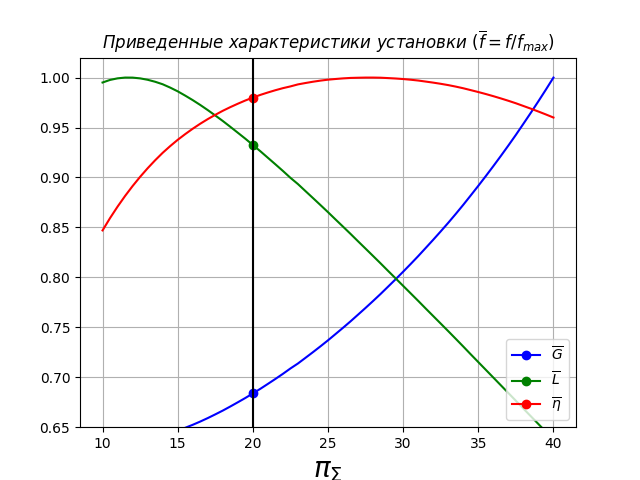
\includegraphics[scale=0.7]{cycle_eta_plot}
	\caption{Характеристики установки}
	\label{img:cycle_eta_plot}
\end{figure}

Экстремум по КПД достигается при следующих значения функций:
\begin{center}
	\begin{tabular}{|c|c|c|c|c|}
	\hline
		$G, кг/с$ & $N_e, Вт/кг$ & $\eta_e$ & $\pi_{кнд}$ & $\pi_{квд}$ \\ \hline
		$60,1$ &
		$0,272 \cdot 10^6$ &
		$0,393$ &
		$5,3$ &
		$5,3$ \\ \hline
	\end{tabular}
\end{center}

Экстремум по удельной мощности достигается при следующих значениях функций:
\begin{center}
	\begin{tabular}{|c|c|c|c|c|}
	\hline
		$G, кг/с$ & $N_e, Вт/кг$ & $\eta_e$ & $\pi_{кнд}$ & $\pi_{квд}$ \\ \hline
		$49,4$ &
		$0,331 \cdot 10^6$ &
		$0,346$ &
		$3,4$ &
		$3,4$ \\ \hline
	\end{tabular}
\end{center}

В связи с высокой температурой за камерой сгорания, для изготовления лопаточных венцов турбины высокого давления требуется
использование крайне дорогих материалов и применение интенсивного охлаждения. Поэтому уменьшение количества ступеней
турбины высокого давления является актуальной технико-экономической задачей. Опираясь на данные вариантного расчета,
можно сказать, что применение в данной схеме двуступенчатой турбины высокого давления приведет к недогрузке
обеих ступеней, а, следовательно, к излишним расходам на материалы. В связи с этим в данной работе принимается
$\pi_{\sum} = 19,0$, $\pi_{кнд} = 4,8$, $\pi_{квд} = 4,0$,
что позволит создать эффективную одноступенчатую турбину высокого давления.

Ниже представлен расчет цикла ГТА при $\pi_{кнд} = 4,8$, $\pi_{квд} = 4,0$.
    \subsection{Расчет цикла}
В данном расчете учет изменения теплофизических свойств рабочего тела в зависимости от его температуры производился
путем итерирования на каждом этапе расчета до тех пор, пока изменение искомого теплофизического свойства (теплоемкости или
показателя адиабаты) не составляло менее 0.1\% в сравнении с результатами предыдущей итерации. Ниже везде используются
значения теплофизический свойств на последнем этапе итерационных расчетов.

\begin{enumerate}
	\item Определим давление за входным устройством:
		$$p_{вх}^* = \sigma_{вх}  p_a = 0,98 \cdot 0,100 = 0,098 \/\ МПа$$
	\item Определим давление за КНД:
		$$p_{кнд}^* = \pi_{кнд} p_{вх}^* = 4,8 \cdot 0,098 = 0,466 \/\ МПа$$
	\item Определим адиабатический КПД КНД $\eta_{кнд}$, принимая показатель адиабаты воздуха $k_{в \/\ кнд} = 1,40$:
	    $$
	    	\eta_{кнд} = \frac{
		        \pi_{кнд}^\frac{
		            k_{в \/\ кнд} - 1
		        }{
		            k_{в \/\ кнд}
	            } - 1
		    }{
		        \pi_{кнд}^\frac{
		            k_{в \/\ кнд} - 1
	            }{
	                k_{в \/\ кнд} \cdot \eta_{пол \/\ кнд}
	            } - 1
		    } = \frac{
	            4,8^\frac{
	                1,40 - 1
	            }{
	                1,40
	            } - 1
	        }{
	            4,8^\frac{
	                1,40 - 1
	            }{
	                1,40 \cdot 0,840
	            } - 1
	        } = 0,80
	    $$
	\item Определим температуру газа за КНД:
		$$T_{КНД}^* = T_a 
		\left[ 
			1 + \frac{
				\pi_к^{
					\frac{
						k_{в \/\ кнд} - 1
					}{
						k_{в \/\ кнд}
					}
				} - 1
			}{
				\eta_{кнд}
			}
		\right] =
			288,0 
		\left[
			1 + \frac{
				{4,8}^{
					\frac{
						1,40 - 1
					}{
						1,40
					}
				} - 1
			}{
				0,80
			}
		\right] = 490,0 \/\ К$$
	\item Используя найденный показатель адиабаты воздуха, определим теплоемкость воздуха в процессе сжатия воздуха в КНД:
		$$c_{pв \/\ кнд} = \frac{
			k_{в \/\ кнд}
		}{
			k_{в \/\ кнд} - 1
		} R_в = \frac{
			1,40
		}{
			1,40 - 1
		} \cdot 287,0 = 1012,1 \/\ Дж/(кг \cdot К)$$
	\item Определим работу КНД:
		$$L_{КНД} = c_{pв \/\ кнд} \left( T_{кнд}^* - T_a \right) =
			1012,1 \cdot \left(490,0 - 288,0\right) =
			0,204 \cdot 10^6 \/\ Дж/кг $$
	\item Определим давление перед КВД:
		$$p_{0 \/\ квд}^* = \sigma_{кнд} p_{кнд}^* = 0,98 \cdot 0,466 = 0,456 \/\ МПа$$
	\item Определим давление за КВД:
		$$ p_{квд}^* = \pi_{квд} p_{0 \/\ квд}^* = 4,0 \cdot 0,456 = 1,825 \/\ МПа $$
	\item Определим адиабатический КПД КВД $\eta_{квд}$, принимая показатель адиабаты воздуха $k_{в \/\ КВД} = 1,37$:
	    $$
	    	\eta_{квд} = \frac{
		        \pi_{квд}^\frac{
		            k_{в \/\ квд} - 1
		        }{
		            k_{в \/\ квд}
	            } - 1
		    }{
		        \pi_{кнд}^\frac{
		            k_{в \/\ квд} - 1
	            }{
	                k_{в \/\ квд} \cdot \eta_{пол \/\ квд}
	            } - 1
		    } = \frac{
	            4,0^\frac{
	                1,37 - 1
	            }{
	                1,37
	            } - 1
	        }{
	            4,0^\frac{
	                1,37 - 1
	            }{
	                1,37 \cdot 0,820
	            } - 1
	        } = 0,78
	    $$
	\item Определим температуру газа за КВД:
		$$T_{квд}^* = T_{кнд}^*
		\left[ 
			1 + \frac{
				\pi_к^{
					\frac{
						k_в - 1
					}{
						k_в
					}
				} - 1
			}{
				\eta_{квд}
			}
		\right] =
			490,0 
		\left[
			1 + \frac{
				{4,0}^{
					\frac{
						1,37 - 1
					}{
						1,37
					}
				} - 1
			}{
				0,78
			}
		\right] = 784,3 \/\ К$$
	\item Используя найденный показатель адиабаты воздуха, определим теплоемкость воздуха в процессе сжатия воздуха в КВД:
		$$c_{pв \/\ квд} = \frac{
			k_{в \/\ квд}
		}{
			k_{в \/\ квд} - 1
		} R_в = \frac{
			1,37
		}{
			1,37 - 1
		} \cdot 287,0 = 1061,8 \/\ Дж/(кг \cdot К)$$
	\item Определим работу КВД:
		$$L_{квд} = c_{pв \/\ квд} \left( T_{квд}^* - T_{кнд}^* \right) =
			1061,8 \cdot \left(784,3 - 490,0\right) =
			0,313 \cdot 10^6 \/\ Дж/кг $$
	\item Температура газа за камерой сгорания:
		$$T_г^* = 1450 \/\ К$$
	\item Определим относительный расход топлива. Расчет носит итерационный характер. Ниже описана последняя итерация. Теплоемкость продуктов сгорания природного газа рассчитывается через показатель адиабаты и газовую постоянную газа. При этом газовая постоянная и истинный показатель адиабаты рассчитываются как средневзвешенное соответственных характеристик компонентов продуктов. При расчета приняты следующие значения:
	\begin{enumerate} % список значений для расчета удельного расхода топлива
		\item[1)] теплоемкость топлива:
			$$c_{pm} = 2226,0 \/\ Дж / (кг \cdot К);$$
		\item[2)] температура подачи топлива:
			$$T_m = 300,0 \/\ К;$$
		\item[3)] температура определения теплофизических параметров веществ:
			$$T_0 = 300,0 \/\ К;$$
		\item[4)] истинная теплоемкость воздуха перед камерой сгорания:
			$$c_{pв \/\ г}\left( T_{КВД} \right) = 1095,4 \/\ Дж/(кг \cdot К);$$
		\item[5)] истинная теплоемкость воздуха при температуре определения теплофизических параметров веществ:
			$$c_{pв \/\ г}\left( T_0 \right) = 1002,7 \/\ Дж/(кг \cdot К);$$
		\item[6)] низшая теплота сгорания топлива:
			$$Q_н^р = 49030 \cdot 10^3 \/\ Дж / кг;$$
		\item[7)] полнота сгорания:
			$$\eta_г = 0,98;$$
		\item[8)] масса воздуха, необходимая для сжигания 1 кг топлива:
			$$l_0 = 17,3 \/\ кг;$$
	\end{enumerate}
	
	\begin{enumerate}
		\item Зададимся коэффициентом избытка воздуха: $$\alpha = 3,32;$$
		\item Теплоемкость продуктов сгорания природного газа $c_{pг \/\ г}$ при данном значении коэффициента избытка воздуха при температуре $T_г$ составляет:
			$$c_{pг \/\ г}\left( T_г \right) = 1222,3 \/\ Дж/(кг \cdot К);$$
		\item Теплоемкость продуктов сгорания природного газа $c_{pг \/\ г}$ при данном значении коэффициента избытка воздуха при температуре $T_0$ составляет:
			$$c_{pг \/\ г}\left( T_0 \right) = 995,0 \/\ Дж / (кг \cdot К);$$
		\item Определим относительный расход топлива:
			$$
				a = c_{pг \/\ г} \left( T_г \right) T_г - c_{pв \/\ г} \left( T_{квд} \right) T_{квд} = 
			$$
			$$
				= 1222,3 \cdot 1450,0 -
				1222,3 \cdot 784,310 = 
				0,913 \cdot 10^6 \/\ Дж/кг
			$$
			$$
				b = \left(
					c_{pг \/\ г}\left( T_0 \right) - c_{pв \/\ г}\left( T_0 \right) = 
				\right) T_0 = 
			$$
			$$
				= \left(
					995,0 - 1002,7
				\right) \cdot 300,0 = 
				-2,327 \cdot 10^3 \/\ Дж/кг
			$$
			$$
				c = c_{pг \/\ г} \left( T_г \right) T_г - c_{pг \/\ г} \left( T_0 \right) T_0 = 
			$$
			$$
				= 1222,3 \cdot 1450,0 -
				995,0 \cdot 300,0 = 
				1,474 \cdot 10^6 \/\ Дж/кг
			$$
			$$
				d = c_{pm} \left( T_m - T_0 \right) = 
			$$
			$$
				= 2226,0 \left( 300,0 - 300,0 \right) =
				0 \/\ Дж/кг
			$$
			$$g_m = \frac{G_m}{G_в^г} =
				\frac{
					a - b
				}{
					Q_н^р \eta_г -
					c + d
				} = 
			$$
			$$
				= \frac{
					0,913 \cdot 10^6 + 2,327 \cdot 10^3
				}{
					49030 \cdot 10^3 \cdot 0.98 -
					1473,793 \cdot 10^6 + 0
				} = 0,017
			$$
		\item Определим коэффициент избытка воздуха:
			$$\alpha^\prime = \frac{1}{g_m l_0} =
		\frac{1}{0,017 \cdot 17,3} = 3,32$$
	\end{enumerate}

	\item Определим удельный расход через ТВД:
		$$g_{твд} = \left( 1 + g_m \right) \left( 1 - g_{ут \/\ твд} - g_{охл \/\ твд} \right) = $$
		$$
		= \left(
		    1 + 0,017
		\right) \left(
		    1 - 0,010 -
		    0,100
        \right) = 1,027$$
	\item Определим удельную работу ТВД:
		$$L_{твд} = \frac{L_{квд}}{g_{твд}\eta_{м \/\ вд}} = \frac{
			0,313 \cdot 10^6
		}{
			1,027 \cdot 0,990
		} = 0,280 \cdot 10^6 \/\ Дж/кг$$
	\item Определим давление газа перед ТВД:
		$$p_{г}^* = p_{тнд}^* \sigma_г = 1,825 \cdot 0,99 = 1,807 \/\ МПа$$
	\item Определим среднюю теплоемкость газа в процессе расширения газа в турбине, принимая показатель адиабаты газа $k_{г \/\ твд} = 1,32$:
		$$c_{pг \/\ твд} = \frac{k_{г \/\ твд}}{k_{г \/\ твд} - 1} R_г =
			\frac{
				1,32
			}{
				1,32 - 1
			} \cdot 291,0 = 1206,6 \/\ Дж/(кг \cdot К) $$
	\item Определим давление воздуха за ТВД:
		$$p_{твд}^* = p_г^*
			\left[
				1 - \frac{L_{твд}}{c_{pг \/\ твд} T_г \eta_{твд}}
			\right] ^ \frac{k_{г \/\ твд}}{k_{г \/\ твд} - 1} =
		$$
		$$
			= 1,807
			\left[
				1 - \frac{0,313 \cdot 10^6}
				{1206,6 \cdot 1450,0 \cdot 0,880}
			\right] ^ \frac{1,32}{1,32 - 1} =
			 0,787 \/\ МПа
		$$
	\item Определим температуру газа за ТВД:
	 	$$
	 		T_{твд}^* = T_г^*
			\left\lbrace
			 	1 -
			 	\left[
			 		1 -
			 			\left(
			 				\frac{p_{твд}^*}{p_г^*}
			 			\right) ^ \frac{k_{г \/\ твд}}{k_{г \/\ твд} - 1}
			 	\right] \eta_{ТВД}
			\right\rbrace =
		$$
		$$
			= 1450,0
			\left\lbrace
			 	1 -
			 	\left[
			 		1 -
			 			\left(
			 				\frac{0,787}{1,807}
			 			\right) ^ \frac{1,32}{1,32 - 1}
			 	\right] \cdot 0,880
			\right\rbrace = 1218,1 \/\ К
		$$
	\item Определим давление перед ТНД:
		$$p_{0 \/\ тнд}^* = p_{твд}^*\sigma_{твд} = 0,787 \cdot 0,98 = 0,771 \/\ МПа$$

	\item Определим удельный расход через ТНД:
		 $$g_{тнд} = g_{твд} \left( 1 - g_{ут \/\ тнд} - g_{охл \/\ тнд} + g_{охл \/\ твд}\right) = $$
		 $$=1,027 \cdot
		 	\left(
		 	    1 - 0,010 -
		 	    0,000 +
		 	    0,100
		 	\right) = 1,037$$
	\item Определим удельную работу ТНД:
		$$L_{тнд} = \frac{L_{кнд}}{g_{тнд}\eta_{м \/\ нд}} = \frac{
			0,204 \cdot 10^6
		}{
			1,037 \cdot 0,99
		} = 0,199 \cdot 10^6 \/\ Дж/кг$$
	\item Определим среднюю теплоемкость газа в процессе расширения газа в ТНД, принимая показатель адиабаты газа $k_{г \/\ тнд} = 1,33$:
		$$c_{pг \/\ тнд} = \frac{k_{г \/\ тнд}}{k_{г \/\ тнд} - 1} R_г =
			\frac{
				1,33
			}{
				1,33 - 1
			} \cdot 291,0 = 1178,1 \/\ Дж/(кг \cdot К) $$
	\item Определим давление воздуха за ТНД:
		$$
			p_{тнд}^* = p_{0 \/\ тнд}^*
				\left[
					1 - \frac{L_{тнд}}{c_{pг \/\ тнд} T_г \eta_{тнд}}
				\right] ^ \frac{k_{г \/\ тнд}}{k_{г \/\ тнд} - 1} =
		$$
		$$
			= 0,771
				\left[
					1 - \frac{
						0,204 \cdot 10^6
					}
					{
						1178,1 \cdot 1218,1 \cdot 0,90
					}
				\right] ^ \frac{1,33}{1,33 - 1} =
				 0,391 \/\ МПа
		$$
	\item Определим температуру газа за ТНД:
	 	$$
	 		T_{тнд}^* = T_{твд}^*
			\left\lbrace
			 	1 -
			 	\left[
			 		1 -
			 			\left(
			 				\frac{p_{тнд}^*}{p_{тнд \/\ 0}^*}
			 			\right) ^ \frac{k_{г \/\ тнд}}{k_{г \/\ тнд} - 1}
			 	\right] \eta_{тнд}
			\right\rbrace =
		$$
		$$
			= 1218,1
			\left\lbrace
			 	1 -
			 	\left[
			 		1 -
			 			\left(
			 				\frac{0,391}{0,771}
			 			\right) ^ \frac{1,33}{1,33 - 1}
			 	\right] \cdot 0,90
			\right\rbrace = 1049,1 \/\ К
		$$
	\item Определим давление перед свободной турбиной:
		$$p_{0 \/\ тс}^* = p_{тнд}^*\sigma_{тнд} = 0,391 \cdot 0,98 = 0,384 \/\ МПа$$
	\item Определим удельный расход через силовую турбину:
	    $$g_{тс} = g_{тнд} \left( 1 - g_{ут \/\ тс} - g_{охл \/\ тс} \right) =
            1,037 \cdot
            \left(
                1 - 0,010 -
                0,000
            \right) = 1,027$$
    \item Определим давление торможения на выходе из свободной турбины $p_{тс}^*$:
		$$p_{тс}^* = p_a / \sigma_{вых} = 0,100 \cdot 0,93 = 0,108 \/\ МПа$$
	\item Зададим значение приведенной скорости на выходе из свободной турбины:
		$$\lambda_{вых} = 0,30$$
	\item Определим статическое давление на выходе из свободной турбины, принимая показатель адиабаты газа на выходе из свободной турбины $k_{тс \/\ вых} = 1,36$:
		$$p_{тс} = p_{тс}^* \cdot \pi \left( \lambda_{вых}, \/\ k_{тс \/\ вых} \right)
        =
			0,108
			\cdot \pi \left( 0,30, \/\ 1,36 \right)
        = 0,102 \/\ МПа$$
	\item Определим статическую температуру на выходе из свободной турбины, принимая показатель адиабаты газа $k_{г \/\ тс} = 1,35$::
		$$
			T_{тс} = T_{тнд}^*
			\left\lbrace
			 	1 -
			 	\left[
			 		1 -
			 			\left(
			 				\frac{p_{0 \/\ тс}^*}{p_{тс}}
			 			\right) ^ \frac{k_{г \/\ тс}}{k_{г \/\ тс} - 1}
			 	\right] \eta_{тс}
			\right\rbrace =
		$$
		$$
			= 1049,1
			\left\lbrace
			 	1 -
			 	\left[
			 		1 -
			 			\left(
			 				\frac{
			 					0,384
			 				}{
			 					0,102
			 				}
			 			\right) ^ \frac{1,35}{1,35 - 1}
			 	\right] \cdot 0,92
			\right\rbrace = 769,6 \/\ К
		$$
	\item Определим температуру торможения на выходе из силовой турбины:
		$$T_{тс}^* = 
			\frac{T_{тс}}{\tau\left( \lambda_{вых}, \/\ k_{тс \/\ вых} \right)} =
			\frac{T_{тс}}{\tau\left( 0,30, \/\ 1,36 \right)} =
			= 780,2 \/\ К$$
	\item Определим значение теплоемкости газа в свободной турбине:
		$$c_{p \/\ тс} = 
			\frac{k_{г \/\ тс}}{k_{г \/\ тс} - 1} = 
			\frac{1,35}{1,35 - 1} = 1133,2 \/\ Дж / \left( кг \cdot К \right)$$
	\item Определим удельную работу силовой турбины:
		$$L_{тс} = c_{p \/\ тс} \left( T_{тнд}^* - T_{тс}^* \right) = 
			1133,2 \cdot \left( 1049,1 - 780,2 \right) =
			0,305 \cdot 10^6\/\ Дж/кг$$
	\item Определим удельную работу ГТД:
		$$L = L_{тс} \/\ g_{тс} =
			0,30 \cdot 10^6 \cdot 1,027 =
			0,305 \cdot 10^6 Дж/кг$$
	\item Определим экономичность ГТД:
		$$C_e = \frac{3600}{N_{e уд}} g_{тс} =
			\frac{3600}{0,305 \cdot 10^6} \cdot 1,03 =
			0,192 \cdot 10^{-3} кг/\left( кВт/ч \right)$$
	\item Определим КПД ГТД:
		$$\eta_e = \frac{3600}{C_e Q_н^р} =
			\frac{3600}{0,192 \cdot 10^{-3} \cdot 49,030 }
			= 0,382$$
	\item Определим потребную мощность ГТД:
		$$
			N = N_e / \eta_р = 16000 \cdot 10^3 \cdot \ 0,98 = 16327 \cdot 10^3 \/\ Вт
		$$
	\item Определим расход воздуха:
		$$G_в = \frac{N}{L} =
			\frac{16327 \cdot 10^3}{0,305 \cdot 10^6} =
			51,1 \/\ кг/с$$
\end{enumerate}
    \section{Расчет компрессора низкого давления по средней линии}

Для в данной работе детально представлен расчет первой ступени КНД по средней линии тока. Параметры остальных ступеней КНД и КВД представлены в табличном виде.

Зададим параметры, необходимы для расчета КНД по средней линии тока:
Исходные данные:
\begin{center}
	\begin{longtable}{|p{7cm}|c|c|c|}
		\hline
		\textbf{Величина} & \textbf{Обозначение} & \textbf{Размерность} & \textbf{Значение} \\ \hline
		\endhead
		Начальная температура воздуха & $T_1$ & К & $288.0$ \\ \hline
		Начальное давление воздуха & $p_1$ & $10^6 \/\ Па$ & $0.098$ \\ \hline
		Частота вращения вала & $n$ & об/мин & $9500$ \\ \hline
		Коэффициент напора текущей ступени & $\overline{H_{тi}}$ & - & $0.284$ \\ \hline
		Коэффициент напора следующей ступени & $\overline{H_{т \/\ i+1}}$ & - & $0.302$ \\ \hline
		Реактивность текущей ступени & $R_{i}$ & - & $0.500$ \\ \hline
		Реактивность следующей ступени & $R_{i+1}$ & - & $0.500$ \\ \hline
		Коэффициент работы & $k_H$ & - & $0.99$ \\ \hline
		КПД ступени & $\eta_{ад}^*$ & - & $0.817$ \\ \hline
		Безразмерная осевая скорость на входе в ступень & $\overline{c_a}$ & - & $0.50$ \\ \hline
		Относительный диаметр втулки на входе в ступень & $\overline{d_1}$ & - & $0.440$ \\ \hline
		Угол наклона внутреннего обвода проточной части & $\gamma_{в}$ & $\degree$ & 8.0 \\ \hline
		Угол наклона наружного обвода проточной части & $\gamma_{н}$ & $\degree$ & -8.0 \\ \hline
		Удлинение лопатки ротора & $\overline{b_{aр}}$ & - & 3.6 \\ \hline
		Удлинение лопатки статора & $\overline{b_{aс}}$ & - & 4.4 \\ \hline
		Относительная ширина зазора за лопатками ротора & $\delta_р$ & - & 0.10 \\ \hline
		Относительная ширина зазора за лопатками статора & $\delta_с$ & - & 0.10 \\ \hline
	\end{longtable}
\end{center}


\begin{enumerate}
	\item Определим окружную скорость на периферии рабочих лопаток на входе в ступень:
		$$
			u_к = \frac{\pi D_1 n}{60} = \frac{\pi \cdot 0.691 \cdot 9500}{60} = 343.67 \/\ м/с.
		$$
	\item Определим теоретический напор ступени:
		$$
			H_т = 
				\overline{H_{тi}} \cdot u_{кi}^2 = 
				0.284 \cdot 343.67^2 = 0.336 \cdot 10^5 \/\ Дж/кг.
		$$ 
	\item Определим действительную работу сжатия:
		$$
			L_z = 
				k_H \cdot H_т = 
				0.99 \cdot 0.336 \cdot 10^5 = 0.333 \cdot 10^5 \/\ Дж/кг.
		$$
	\item Определим адиабатическую работу сжатия:
		$$
			H_{ад} = L_z \cdot \eta_{ад}^* = 
				0.333 \cdot 10^5 \cdot 0.817 = 0.272 \cdot 10^5 \/\ Дж/кг.
		$$
	\item Определим повышение полной температуры в ступени:
		$$
			\Delta T^* = L_z / c_{pв} = 
				0.333 \cdot 10^5 / 1003.0 = 32.9 \/\ К.
		$$
	\item Определим степень повышения полного давления:
		$$
			\pi^* = 
			\left[ 
				1 + \frac{H_{ад}}{c_{pв} T_1^*}
			\right]^\frac{k_в}{k_в - 1} = 
			\left[ 
				1 + \frac{0.272 \cdot 10^5}{1003.0 \cdot 288.0}
			\right]^\frac{1.40}{1.40 - 1} = 1.37.
		$$
	\item Определим полное давление на выходе из ступени:
		$$
			p_3^* = p_1^* \cdot \pi^* = 
				0.098 \cdot 10^6 \cdot 1.37 = 
				0.134 \cdot 10^6  \/\ Па.
		$$
	\item Определим критическую скорость потока на входе в ступень:
		$$
			a_{кр1} = \sqrt{
				\frac{2 k_в}{k_в + 1} R_в T_1^*
			} = \sqrt{
				\frac{
					2 \cdot 1.40
				}{
					1.40 + 1
				} \cdot 287.0 \cdot 288.0
			} = 310.65 \/\ м/с.
		$$ 	
	\item Определим критическую скорость потока на выходе из ступени:
		$$
			a_{кр3} = \sqrt{
				\frac{2 k_в}{k_в + 1} R_в T_3^*
			} = \sqrt{
				\frac{
					2 \cdot 1.40
				}{
					1.40 + 1
				} \cdot 287.0 \cdot 320.9
			} = 327.78 \/\ м/с.
		$$ 	
	\item Определим относительный средний радиус на входе в ступень:
		$$
			\overline{r_{ср1}} = 
				\sqrt{\frac{1 + \overline{d_1}}{2}} = 
				\sqrt{\frac{1 + 0.44}{2}} = 0.85.
		$$
	\item Определим безразмерную окружную составляющую абсолютной скорости на входе в ступень:
		$$
			\overline{c_{u1}} = 
				\overline{r_{ср1}} \cdot \left( 
					1 - R_{ср \ i}
				\right) - 
				\frac{
					\overline{H_т}
				}{
					2 \overline{r_{ср1}}
				} = 
				0.85 \cdot
				\left( 
					1 - 0.50
				\right) - 
				\frac{
					0.28
				}{
					2 \cdot 0.85
				} = 0.26.
		$$
	\item Определим направление абсолютной скорости на входе в ступень:
		$$
			\alpha_1 = \arctan{\frac{
				\overline{c_{a1}}
			}{
				\overline{c_{u1}}
			}} = \arctan{\frac{
				0.50
			}{
				0.26
			}} = 62.8 \degree.
		$$
	\item Определим величину осевой скорости на входе в ступень:
		$$
			c_{a1} = u_к \cdot \overline{c_a} = 343.67 \cdot 0.50 = 171.83 \/\ м/с.
		$$
	\item Определим приведенную скорость на входе в ступень:
		$$
			\lambda_1 = 
				\frac{
					c_{a1}
				}{
					\sin{\alpha_1} \cdot a_{кр1}
				} = 
				\frac{
					171.83
				}{
					\sin{
						62.8 \degree
					} \cdot 310.65
				} = 0.62.
		$$
	\item Величина функции $Q\left( 
		\lambda, k_в, R_в
	\right) = \frac{
		m\left( k_в \right) q\left( \lambda \right)
	}{
		\sqrt{R_в}
	}$, соответствующая полученному значению приведенной скорости равна:
		$$
			Q\left( \lambda_1, k_в, R_в \right) = 0.03 \left( \frac{Дж}{кг \cdot К} \right)^{0.5}.
		$$
	\item Определим кольцевую площадь на входе в ступень:
		$$
			F_1 = 
			\frac{
				G \sqrt{T_1^*}
			}{
				p_1^* Q\left( \lambda_1, k_в, R_в\right) \sin{\alpha_1}
			} = 
			\frac{
				52.2 \cdot \sqrt{
					288.0
				}
			}{
				0.10 \cdot 10^6 \cdot 
				0.03 \cdot \sin{62.8 \degree}
			} = 0.30 \/\ м^2.
		$$
	\item Определим внешний и внутренний диаметры на входе в ступень:
		$$
			D_1 = \sqrt{
				\frac{4}{\pi} \cdot 
				\frac{1}{1 - \overline{d}^2} \cdot
				F_1
			} = 
			\sqrt{
				\frac{4}{\pi} \cdot 
				\frac{1}{1 - 0.44} \cdot
				0.30
			} = 0.691 \/\ м,	
		$$
		$$
			d_1 = D_1 \cdot \overline{d_1}^2 = 
				0.691 \cdot 0.440 = 
				0.304 \/\ м.
		$$
	\item Определим ширину ступени:
		$$
			x_{ступ} = 
				D_1 \cdot \frac{
					1 - \overline{d_1}
				}{2} \cdot \left(
					\frac{
						1 + \overline{\delta_р}
					}{
						\overline{b_{aр}}
					} + 
					\frac{
						1 + \overline{\delta_с}
					}{
						\overline{b_{aс}}
					}
				\right) =
		$$
		$$
				= 0.691 \cdot \frac{
					1 - 0.440
				}{2} \cdot \left(
					\frac{
						1 + 0.10
					}{
						3.6
					} + 
					\frac{
						1 + 0.10
					}{
						4.4
					}
				\right) = 0.103 \/\ м.
		$$
	\item Определим внешний и внутренний диаметры на выходе из ступени:
		$$
			D_3 = 
				D_1 + 2 \cdot x_{ступ} \tan{\gamma_{н}} = 
				0.691 + 2 \cdot 
				0.103 \cdot \tan{-8.0 \degree} =
				0.662 \/\ м, 
		$$
		$$
			d_3 =
				d_1 + 2 \cdot x_{ступ} \tan{\gamma_{в}} = 
				0.304 + 2 \cdot 
				0.103 \cdot \tan{8.0 \degree} =
				0.333 \/\ м 
		$$
	\item Определим кольцевую площадь на выходе из ступени:
		$$
			F_3 = 
				\frac{\pi}{4} \left( D_3^2 - d_3^2 \right) = 
				\frac{\pi}{4} \left( 
					0.662^2 - 0.333^2
				\right) = 0.257 \/\ м^2.
		$$
	\item Определим относительный диаметр втулки на выходе из ступени:
		$$
			\overline{d_3} = \frac{d_3}{D_3} = 
			\frac{0.333}{0.662} = 0.503.
		$$
	\item Определим относительный средний радиус на выходе из ступени:
		$$
			\overline{r_{ср \ 3}} = \sqrt{
				\frac{1 + \overline{d_3}^2}{2}
			} = 
			\sqrt{
				\frac{1 + 0.503^2}{2}
			} = 0.867.
		$$ 
	\item Определим безразмерную окружную составлющую абсолютной скорости на выходе из ступени:
		$$
			\overline{c_{u3}} = 
				\overline{r_3} \cdot \left( 
					1 - R_{ср \ i+1}
				\right) - 
				\frac{
					\overline{H_{т \ i+1}}
				}{
					2 \cdot \overline{r_{ср \ 3}}
				} =
				0.87 \cdot \left( 
					1 - 0.50
				\right) - 
				\frac{
					0.30
				}{
					2 \cdot 0.87
				} = 0.259. 
		$$
	\item Для определения приведенной скорости на выходе из ступени, численно решим уравнение:
		$$
			\frac{
				Q \left( 
				\lambda_3, k_в, R_в
			\right)
			}{
				\lambda_3
			} = \frac{
				a_{кр3}
			}{
				c_{a3}
			} \cdot \frac{
				G
			}{
				F_3
			} \cdot \frac{
				\sqrt{T_3^*}
			}{
				p_3^*
			}
		$$.
		Получим значение приведенной скорости на выходе:
		$$
			\lambda_3 = 0.56.
		$$
	\item Определим направление потока в абсолютном движении на выходе из ступени:
		$$
			\alpha_3 = \arcsin{
				\frac{
					c_{a3}
				}{
					\lambda_3 \cdot a_{кр \ 3}
				}
			} = \arcsin{
				\frac{
					158.78
				}{
					0.56 \cdot 327.78
				}
			} = 60.7 \degree.
		$$
	\item Определим безразмерную окружную составляющую абсолютной скорости на выходе из рабочего колеса:
		$$
			\overline{c_{u2}} = \frac{1}{\overline{r_{ср \ 2}}} 
			\left( 
				\overline{
					H_т
				} + \overline{c_{u1}} \overline{r_{ср1}}
			\right) = 
			\frac{1}{0.86} 
			\left( 
				0.28 + 
				0.26 \cdot 0.86
			\right) = 0.48.
		$$
	\item Определим углы потока в относительном движении:
		$$
			\beta_1 = \arctan{
				\frac{
					\overline{c_{a1}}
				}{
					\overline{r_{ср1}} - \overline{c_{u1}}
				}
			} = \arctan{
				\frac{
					0.50
				}{
					0.85 - 
					0.26
				}
			} = 40.2 \degree.
		$$
		$$
			\beta_2 = \arctan{
				\frac{
					\overline{c_{a2}}
				}{
					\overline{r_{ср2}} - \overline{c_{u2}}
				}
			} = \arctan{
				\frac{
					0.48
				}{
					0.86 - 
					0.58
				}
			} = 62.2\degree,
		$$
	\item Определим направление потока в абсолютном движении после рабочего колеса:
		$$
			\alpha_2 = \arctan{
				\frac{
					\overline{c_{a2}}
				}{
					\overline{c_{u2}}
				}
			} = \arctan{
				\frac{
					0.48
				}{
					0.58
				}
			} = 39.4\degree.
		$$
	\item Определим относительную скорость на среднем радиусе на входе в рабочее колесо:
		$$
			w_1 = \frac{c_{a1}}{\sin{\beta_1}} =
				\frac{
					171.8
				}{\sin{
					40.2
				}} = 266.3 \/\ м/с. 
		$$
	\item Определим относительную скорость на среднем радиусе на входе в НА:
		$$
			c_2 = \frac{
				c_{a2}
			}{
				\sin{\alpha_2}
			} = \frac{
				165.3
			}{
				\sin{
					39.4 \degree
				}
			} = 260.22 \/\ м/с.
		$$
\end{enumerate}



% section расчет_компрессора_низкого_давления_по_средней_линии (end)
    \begin{landscape}
	\begin{center}
		\begin{longtable}{|c|c|c|c|c|c|c|c|c|c|}
			\hline
			\textbf{№} & 
			\textbf{Наименование} & 
			\textbf{Размерность} & 
			\textbf{1} & 
			\textbf{2} &
			\textbf{3} &
			\textbf{4} &
			\textbf{5} &
			\textbf{6} &
			\textbf{7} \\\hline
			\endhead
			
				1 & $H_т$ & $10^5 \cdot Дж/кг$ & 0.336 & 0.327 & 0.312 & 0.290 & 0.277 & 0.265 & 0.256 \\\hline
			
				2 & $L_z$ & $10^5 \cdot Дж/кг$ & 0.333 & 0.324 & 0.309 & 0.287 & 0.274 & 0.262 & 0.253 \\\hline
			
				3 & $H_{ад}$ & $10^5 \cdot Дж/кг$ & 0.272 & 0.270 & 0.257 & 0.238 & 0.227 & 0.216 & 0.207 \\\hline
			
				4 & $\Delta T$ & $К$ & 32.9 & 31.9 & 30.3 & 28.1 & 26.6 & 25.3 & 24.3 \\\hline
			
				5 & $\pi^*$ & - & 1.369 & 1.325 & 1.278 & 1.234 & 1.206 & 1.182 & 1.165 \\\hline
			
				6 & $p_1^*$ & $10^6 \cdot Па$ & 0.098 & 0.134 & 0.178 & 0.227 & 0.280 & 0.338 & 0.400 \\\hline
			
				7 & $p_3^*$ & $10^6 \cdot Па$ & 0.134 & 0.178 & 0.227 & 0.280 & 0.338 & 0.400 & 0.466 \\\hline
			
				8 & $a_{кр1}$ & $м/с$ & 310.65 & 327.90 & 343.82 & 358.30 & 371.20 & 383.03 & 393.94 \\\hline
			
				9 & $a_{кр3}$ & $м/с$ & 327.78 & 343.64 & 358.05 & 370.81 & 382.46 & 393.16 & 403.16 \\\hline
			
				10 & $\overline{r_{ср1}}$ & - & 0.849 & 0.867 & 0.885 & 0.904 & 0.914 & 0.924 & 0.931 \\\hline
			
				11 & $\overline{c_{u1}}$ & - & 0.257 & 0.271 & 0.277 & 0.289 & 0.291 & 0.298 & 0.302 \\\hline
			
				12 & $\alpha_1$ & $\degree$ & 62.8 & 60.7 & 60.4 & 61.7 & 61.5 & 61.6 & 61.4 \\\hline
			
				13 & $\lambda_1$ & - & 0.62 & 0.56 & 0.52 & 0.52 & 0.49 & 0.47 & 0.46 \\\hline
			
				14 & $F_1$ & $м^2$ & 0.302 & 0.257 & 0.215 & 0.174 & 0.153 & 0.134 & 0.120 \\\hline
			
				15 & $D_1$ & м & 0.320 & 0.347 & 0.373 & 0.393 & 0.406 & 0.417 & 0.427 \\\hline
			
				16 & $d_1$ & м & 0.304 & 0.333 & 0.360 & 0.386 & 0.399 & 0.412 & 0.422 \\\hline
			
				17 & $x_{ступ}$ & м & 0.103 & 0.095 & 0.094 & 0.077 & 0.070 & 0.058 & 0.055 \\\hline
			
				18 & $D_3$ & м & 0.662 & 0.635 & 0.609 & 0.595 & 0.583 & 0.575 & 0.567 \\\hline
			
				19 & $d_3$ & м & 0.675 & 0.648 & 0.622 & 0.602 & 0.589 & 0.579 & 0.571 \\\hline
			
				20 & $F_3$ & $м^2$ & 0.257 & 0.215 & 0.174 & 0.153 & 0.134 & 0.120 & 0.107 \\\hline
			
				21 & $\overline{d_3}$ & - & 0.503 & 0.566 & 0.634 & 0.671 & 0.706 & 0.734 & 0.761 \\\hline
			
				22 & $\overline{r_{ср3}}$ & - & 0.867 & 0.885 & 0.904 & 0.914 & 0.924 & 0.931 & 0.938 \\\hline
			
				23 & $\overline{c_{u3}}$ & - & 0.259 & 0.266 & 0.277 & 0.284 & 0.292 & 0.298 & 0.304 \\\hline
			
				24 & $\lambda_3$ & - & 0.556 & 0.517 & 0.515 & 0.487 & 0.474 & 0.459 & 0.453 \\\hline
			
				25 & $\alpha_3$ & $\degree$ & 60.7 & 60.4 & 61.7 & 61.5 & 61.6 & 61.4 & 61.6 \\\hline
			
				26 & $\overline{c_{u2}}$ & - & 0.58 & 0.61 & 0.62 & 0.64 & 0.63 & 0.64 & 0.64 \\\hline
			
				27 & $\beta_1$ & $\degree$ & 40.2 & 39.0 & 38.8 & 41.1 & 40.6 & 41.3 & 41.3 \\\hline
			
				28 & $\beta_2$ & $\degree$ & 62.2 & 62.7 & 63.3 & 63.6 & 62.8 & 62.5 & 62.3 \\\hline
			
				29 & $\alpha_2$ & $\degree$ & 39.4 & 37.8 & 38.8 & 39.8 & 40.3 & 40.8 & 41.3 \\\hline
			
				30 & $w_2$ & $м/с$ & 186.88 & 176.16 & 177.38 & 179.29 & 178.89 & 179.13 & 180.19 \\\hline
			
				31 & $c_2$ & $м/с$ & 260.22 & 255.24 & 252.84 & 250.56 & 245.82 & 243.39 & 241.77 \\\hline
			
		\caption{Сводная таблица параметров КНД} \label{tab:lpc-stage-total}
		\end{longtable}
	\end{center}
\end{landscape}

    % \begin{landscape}
	\begin{center}
		\begin{longtable}{|c|c|c|c|c|c|c|c|}
			\caption{Сводная таблица параметров КВД} \label{tab:hpc-stage-total}
			\endfirsthead
			\caption*{\tabcapalign Продолжение таблицы~\thetable}\\[-0.45\onelineskip]
			\hline
			\textbf{№} &
			\textbf{Наименование} &
			\textbf{Размерность} &
			\textbf{1} &
			\textbf{2} &
			\textbf{3} &
			\textbf{4} &
			\textbf{5} \\\hline
			\endhead
			\hline
			\textbf{№} &
			\textbf{Наименование} &
			\textbf{Размерность} &
			\textbf{1} &
			\textbf{2} &
			\textbf{3} &
			\textbf{4} &
			\textbf{5}  \\\hline
			
				1 & $H_т$ & $10^5 \cdot Дж/кг$ & 0.609 & 0.618 & 0.621 & 0.618 & 0.609 \\\hline
			
				2 & $L_z$ & $10^5 \cdot Дж/кг$ & 0.603 & 0.612 & 0.615 & 0.612 & 0.603 \\\hline
			
				3 & $H_{ад}$ & $10^5 \cdot Дж/кг$ & 0.481 & 0.496 & 0.501 & 0.496 & 0.481 \\\hline
			
				4 & $\Delta T$ & $К$ & 57.7 & 57.9 & 57.4 & 56.4 & 54.8 \\\hline
			
				5 & $\pi^*$ & - & 1.387 & 1.354 & 1.320 & 1.287 & 1.254 \\\hline
			
				6 & $p_1^*$ & $10^6 \cdot Па$ & 0.456 & 0.633 & 0.857 & 1.131 & 1.455 \\\hline
			
				7 & $p_3^*$ & $10^6 \cdot Па$ & 0.633 & 0.857 & 1.131 & 1.455 & 1.825 \\\hline
			
				8 & $a_{кр1}$ & $м/с$ & 405.19 & 428.37 & 450.43 & 471.30 & 490.95 \\\hline
			
				9 & $a_{кр3}$ & $м/с$ & 426.92 & 448.49 & 468.87 & 487.95 & 505.72 \\\hline
			
				10 & $\overline{r_{ср1}}$ & - & 0.962 & 0.967 & 0.973 & 0.976 & 0.979 \\\hline
			
				11 & $\overline{c_{u1}}$ & - & 0.000 & 0.310 & 0.312 & 0.315 & 0.320 \\\hline
			
				12 & $\alpha_1$ & $\degree$ & 90.0 & 51.1 & 49.4 & 46.5 & 44.7 \\\hline
			
				13 & $\lambda_1$ & - & 0.42 & 0.49 & 0.46 & 0.42 & 0.39 \\\hline
			
				14 & $F_1$ & $м^2$ & 0.101 & 0.088 & 0.074 & 0.066 & 0.058 \\\hline
			
				15 & $D_1$ & м & 0.587 & 0.601 & 0.612 & 0.621 & 0.628 \\\hline
			
				16 & $d_1$ & м & 0.580 & 0.594 & 0.609 & 0.617 & 0.625 \\\hline
			
				17 & $x_{ступ}$ & м & 0.030 & 0.029 & 0.028 & 0.030 & 0.031 \\\hline
			
				18 & $D_3$ & м & 0.682 & 0.682 & 0.682 & 0.682 & 0.682 \\\hline
			
				19 & $d_3$ & м & 0.682 & 0.682 & 0.682 & 0.682 & 0.682 \\\hline
			
				20 & $F_3$ & $м^2$ & 0.088 & 0.074 & 0.066 & 0.058 & 0.053 \\\hline
			
				21 & $\overline{d_3}$ & - & 0.872 & 0.893 & 0.905 & 0.917 & 0.925 \\\hline
			
				22 & $\overline{r_{ср3}}$ & - & 0.967 & 0.973 & 0.976 & 0.979 & 0.981 \\\hline
			
				23 & $\overline{c_{u3}}$ & - & 0.310 & 0.312 & 0.315 & 0.320 & 0.326 \\\hline
			
				24 & $\lambda_3$ & - & 0.494 & 0.460 & 0.420 & 0.396 & 0.374 \\\hline
			
				25 & $\alpha_3$ & $\degree$ & 51.1 & 49.4 & 46.5 & 44.7 & 42.4 \\\hline
			
				26 & $\overline{c_{u2}}$ & - & 0.34 & 0.66 & 0.66 & 0.66 & 0.66 \\\hline
			
				27 & $\beta_1$ & $\degree$ & 22.6 & 30.3 & 28.9 & 26.7 & 25.7 \\\hline
			
				28 & $\beta_2$ & $\degree$ & 32.3 & 50.0 & 47.9 & 45.6 & 43.7 \\\hline
			
				29 & $\alpha_2$ & $\degree$ & 48.7 & 29.7 & 27.9 & 26.2 & 25.0 \\\hline
			
				30 & $w_2$ & $м/с$ & 314.51 & 209.23 & 201.21 & 194.62 & 190.45 \\\hline
			
				31 & $c_2$ & $м/с$ & 223.30 & 323.56 & 319.54 & 314.84 & 311.11 \\\hline
			
		\end{longtable}
	\end{center}
% \end{landscape}

    \subsection{Поступенчатый расчет турбины}
Для данного проекта выбрана одноступенчатая турбина.
Исходные параметры для поступенчатого расчета турбины приведены в табл. ~\ref{turbine:midline_inlet}.
Расчет проведен по методике ~\cite{gtd_theory_text_book, mikhaltsev_1, mikhaltsev_2}.
\begin{center}
	\begin{longtable}{|p{4cm}|c|c|c|}
		\caption{Исходные параметры поступенчатого расчета турбины}
		\label{turbine:midline_inlet}
		\endfirsthead
		\caption*{\tabcapalign Продолжение таблицы~\thetable}\\[-0.45\onelineskip]
		\hline
		\textbf{Величина} & \textbf{Обозначение} & \textbf{Размерность} & \textbf{Значение} \\ \hline
		\endhead
		\hline
		\textbf{Величина} & \textbf{Обозначение} & \textbf{Размерность} & \textbf{Значение} \\ \hline
			Реактивность ступени & $\rho$ & - & 0,3  \\ \hline
			Радиальный зазор & $\delta_r$ & м & $1,00 \cdot 10^{-3}$ \\ \hline
			Относительная длина лопатки статора & $\left( \frac{l}{D} \right)_1$ & - & $0,107$ \\ \hline
			Удлинение лопатки статора & $\left( \frac{l}{b_a} \right)_{СА}$ & - & $1,70$ \\ \hline
			Удлинение лопатки ротора & $\left( \frac{l}{b_a} \right)_{РК}$ & - & $2,10$ \\ \hline
			Относительная ширина зазора между лопатками ротора и лопатками статора & $\left( \frac{\delta}{b_a} \right)_{СА}$ & - & $0,10$ \\ \hline
			Угол раскрытия на втулке & $\gamma_{в}$ & \degree & $8,0$ \\ \hline
			Угол раскрытия на периферии & $\gamma_{п}$ & \degree & $20,0$ \\ \hline
			Удельная работа турбины & $H_т$ & Дж/кг & $0,341 \cdot 10^6$ \\ \hline
			Коэффициент скорости статора & $\phi$ & - & 0,94 \\ \hline
			Коэффициент скорости ротора & $\psi$ & - & 0,94 \\ \hline
			Направление скорости на выходе из СА & $\alpha_1$ & $\degree$ & 13,0 \\ \hline
			Частота вращения вала турбины & $n$ & $об/мин$ & 12000,0 \\ \hline
	\end{longtable}
\end{center}

Расчет параметров параметров ТВД приведен ниже. Параметры остальных турбин приведены в табл. ~\ref{tab:turbine-stage-total}.
\begin{enumerate}
	\item Определим теплоперепад на сопловом аппарате:
		$$H_с = \left( 1 - \rho \right) H_т =
		\left( 
			1 - 0,3 
		\right) \cdot 0,341 \cdot 10^6 = 
			0,238 \cdot 10^6 \/\ Дж/кг$$
	\item Определим скорость адиабатного истечения из СА:
		$$c_{1 ад} = \sqrt{2 H_с} = 
			\sqrt{2 \cdot 0,238 \cdot 10^6} = 690,5 \/\ м/с$$
	\item Определим скорость действительного истечения из СА:
		$$c_1 = \phi c_{1 ад} =
			0,94 \cdot 690,5 = 651,4 \/\ м/с$$
	\item Определим температуру на выходе из СА:
		$$T_1 = T_г - \frac{c_1^2}{2c_{pг}} =
			1450 - 
			\frac{
				{651,4}^2
			}{
				2 \cdot 1210,3
			} = 1274,7 \/\ К$$
	\item Определим температуру конца адиабатного расширения:
		$$T_1^\prime = T_г - \frac{H_c}{c_{pг}} =
			1450,0 - 
			\frac{
				0,238 \cdot 10^6
			}{
				1210,3
			} = 1255,0 \/\ К$$
	\item Определим давление на выходе из СА:
		$$p_1 = p_г \left( \frac{T_1^\prime}{T_г} \right)^\frac{k_г}{k_г - 1} =
			1,807 \cdot \left(
				 \frac{
				 	1255,0
				 }{
				 	1450,0
				 } 
			\right)^\frac{
				1,32
			}{
				1,32 - 1
			} = 0,991 \/\ МПа$$
	\item Определим плотность газа на выходе из СА:
		$$\rho_1 = \frac{p_1}{R_г T_1} =
			\frac{
				0,991 \cdot 10^6
			}{
				291,0 \cdot 1274,7
			} = 2,67 \/\ кг/м^3$$
	\item Зададим угол на выходе из СА:
		$$\alpha_1 = 13,0 \degree$$
	\item Определим осевую скорость на выходе из СА:
		$$c_{1a} = c_1 \cdot \sin \alpha_1 =
			651,4 \cdot 
			\sin13,0\degree 
			= 146,5 \/\ м/с$$
	\item Определим площадь на выходе из СА:
		$$A_1 = \frac{G}{c_{1a} \rho_1} =
			\frac{
				53,1
			}{
				146,5 \cdot 2,67
			} = 0,13 \/\ м^2$$
	\item Определим средний диаметр турбины на выходе из СА:
	$$D_1 = \sqrt{
		\frac{A_1}{\pi \left( \frac{l}{D} \right)_1}
		} = \sqrt{
			\frac{
				0,13
			}{
				\pi \cdot 0,107
			}
		} = 0,632 \/\ м $$
	\item Определим окружную скорость на среднем диаметре на входе в РК:
		$$u_1 = \frac{\pi D_1 n}{60} = 
			\frac{
				\pi \cdot 0,653 \cdot 12000,0
			}{60} = 398,7 \/\ м/с$$
	\item Определим относительную скорость на входе в РК:
		$$w_1 = \sqrt{c_1^2 + u_1^2 - 2 c_1 u_1 \cos \alpha_1} =$$
		$$
			=\sqrt{
				{651,4}^2 + 
				{398,7}^2 - 
				2 \cdot 651,4 \cdot 398,7 \cdot 
				\cos 13,0 \degree
			} = 277,9 \/\ м/с
		$$
	\item Определим температуру торможения в относительном движении на входе в РК:
		$$T_{w1} = T_1 + \frac{w_1^2}{2c_{p г}} = 
			1274,7 + 
			\frac{
				277,9^2
			}{
				2 \cdot 1194,1
			} = 1306,9 \/\ К$$
	\item Определим давление торможения в относительном движении на входе в РК:
		$$p_{w1} = p_1 \left( \frac{T_{w1}}{T_1} \right)^\frac{k_г}{k_г - 1} =
	 		0,991 \cdot \left( 
	 			\frac{
	 				1306,9
	 			}{
	 				1274,7
	 			} 
	 		\right)^\frac{
	 			1,32
	 		}{
	 			1,32 - 1
	 		} = 1,099 \/\ МПа$$
	 \item Определим теплоперепад на РК:
	 	$$H_л = H_т \rho \frac{T_1}{T_1^\prime} =
	 		0,341 \cdot 10^6 \cdot 0,3 \cdot \frac{
	 			1274,7
	 		}{
	 			1255,0
	 		} = 0,100 \cdot 10^6 \/\ Дж/кг$$
	\item Определим расстояние в осевом направлении между выходными кромками лопаток СА и выходными кромками лопаток РК:
		$$x = \frac{
		 	\frac{\delta_a}{ \left( \frac{l}{b_a} \right)_1 }	+
		 	\frac{1}{\left( \frac{l}{b_a} \right)_2 }
		}{
		 	1 - \frac{\tan \gamma_п + \tan \gamma_в}
		 	{2 \left( \frac{l}{b_a} \right)_2}
		} D_1 \left( \frac{l}{D} \right)_1 =
		\frac{
		 	\frac{
		 		0,10
		 	}{
		 		1,70
		 	}	+
		 	\frac{
		 		1
		 	}{
		 		2,10
		 	} 
		}{
			1 - \frac{
				\tan 20,0 \degree + \tan 8,0 \degree
			}{
				2 \cdot 2,10
			}
		} \cdot 0,632 \cdot 0,107 =
			0,042 \/\ м
		$$
	 \item Определим средний диаметра на выходе из РК:
		 $$D_2 = D_1 + \frac{\tan \gamma_п - \tan \gamma_в}{2} x =
	   		0,632 + 
	   		\frac{
	   			\tan 20,0 \degree - 
	   			\tan 8,0 \degree
	   		}{2} \cdot 0,042 =
   		0,653 \/\ м$$
	 \item Определим длину лопатки на выходе из РК:
		 $$l_2 = 
		 	D_1 \left( \frac{l}{D} \right)_1 + 
		 	\frac{\tan \gamma_п + \tan \gamma_в}{2} x =
	 	$$
	 	$$
	 		= 0,632 \cdot 
		 	0,107 +
		 	\frac{
		 		\tan 20,0 \degree + 
		 		\tan 8,0 \degree
		 	}{2} \cdot 0,042 =
		 		0,078 \/\ м
	 	$$
	 \item Определим относительную длину лопаток на выходе из РК:
		 $$\left( \frac{l}{D} \right)_2 = \frac{l_2}{D_2} = 
		 	\frac{
		 		0,078
		 	}{
		 		0,653
		 	} = 0,120$$
	 \item Определим окружную скорость на среднем диаметре на выходе из РК:
		 $$u_2 = \frac{\pi D_2 n}{60} = 
		 	\frac{
		 		\pi 
		 		\cdot 0,653 
		 		\cdot 12000,0
		 	}{60} = 411,7 \/\ м/с$$
	 \item Определим адиабатическую относительную скорость истечения газа из РК:
	 	$$w_{2 ад} = \sqrt{w_1^2 + 2H_л + \left( u_2^2 - u_1^2 \right)} =$$
	 	$$
	 		= \sqrt{
	 			{277,9}^2 + 
	 			2 \cdot 0,100 \cdot 10^6 + 
	 			\left( {411,7}^2 - {398,7}^2 \right)
	 		} = 535,8 \/\ м/с
	 	$$
	 \item Определим относительную скорость истечения газа из РК:
	 	$$w_2 = \psi w_{2 ад} =
	 		0,94 \cdot 535,8 = 
	 		505,5 \/\ м/с$$
	 \item Определим статическую температуру на выходе из РК:
		 $$
			 T_2 = T_1 + \frac{
			 	\left(
			 		w_1^2  - w_2^2
			 	\right) + \left(
			 		u_2^2 - u_1^2
			 	\right)
			 }{2 c_{p г}} =
		 $$
		 $$
		 	= 1274,7 + \frac{
			 	\left(
			 		{277,9}^2  - {505,5}^2 
			 	\right) + 
			 	\left( 
			 		{398,7}^2  - {411,7}^2
			 	\right)
		 	}{2 \cdot 1194,1} = 
		 		1204,4 \/\ К
		 $$
	 \item Определим статическую температуру при адиабатическом процессе в РК:
		 $$T_2^\prime = T_1 + \frac{
		 	\left(
		 		w_1^2  - w_{2 ад}^2
		 	\right) + 
		 	\left(
		 		u_2^2 - u_1^2
		 	\right)
		 }{2 c_{p г}} =
		$$
		$$
			= 1274,7 + \frac{
			 	\left(
			 		{277,9}^2  - {535,8}^2 
			 	\right) + 
			 	\left( 
			 		{398,7}^2  - {411,7}^2
			 	\right)
			}{2 \cdot 1194,1} = 
			1191,2 \/\ К
		$$
	 \item Определим давление на выходе из РК:
	 	$$p_2 = p_1 
	 		\left( 
	 			\frac{
	 				T_2^\prime
	 			}{
	 				T_1
	 			} 
	 		\right)^{
	 			\frac{
	 				k_г
	 			}{
	 				k_г - 1
	 			}
	 		} =
	 		0,991 
	 		\left( 
	 			\frac{
	 				1191,2
	 			}{
	 				1274,7
	 			} 
	 		\right)^{
	 			\frac{
	 				1,32
	 			}{
	 				1,32 - 1
	 			}
	 		} = 0,751 \/\ МПа$$
	 \item Определим угол в относительном движении на выходе из РК:
	 	$$\beta_2 = \arcsin\frac{c_{2a}}{w_2} = 
	 	\arcsin\frac{
	 		154,6
	 	}{
	 		505,5
	 	} = 17,8 \degree$$
	 \item Определим угол выхода из РК в абсолютном движении:
	 	$$\alpha_2 = \arctan\frac{w_2 \cos \beta_2 - u_2}{c_{2a}} =
	 	\arctan\frac{
	 		505,5 \cdot 
	 		\cos 17,8 \degree - 
	 		411,7
	 	}{
	 		154,6
	 	} = 65,8 \degree$$
	 \item Определим окружную составляющую скорости на выходе из РК:
	 	$$c_{2u} = w_2 \cos \beta_2 - u_2 =
		 	505,5 \cdot 
		 	\cos 17,8 \degree - 
		 	411,7 = 
		 	69,6 \/\ м/с$$
	 \item Определим скорость потока на выходе из РК:
	 	$$c_2 = \sqrt{c_{2u}^2 + c_{2a}^2} = 
	 		\sqrt{
	 			{69,6}^2 + {154,6}^2
	 		} = 169,6 \/\ м/с$$
	 \item Определим степень понижения давления в турбине:
	 	$$\pi_{т} = \frac{p_г}{p_2} = 
	 		\frac{
	 			1,807
	 		}{
	 			0,751
	 		} = 2,41 $$
	 \item Определим осевую составляющую скорости газа за турбиной:
	 	$$c_{2a} = c_2 \sin \alpha_2 = 
	 		169,6 \cdot
	 		\sin 65,8 \degree = 
	 		154,6 \/\ м/с$$
	 \item Определим плотность газа за турбиной:
	 	$$\rho_2 = \frac{G}{\pi \cdot c_{2a} \cdot D_2 \cdot l_2} = 
	 	\frac{
	 		53,1
	 	}{
	 		\pi \cdot 
	 		154,6 \cdot 
	 		0,653 \cdot 
	 		0,078
	 	} = 2,14 \/\ кг/м^3$$
	 \item Определим работу на окружности колеса:
	 $$L_u = c_{1u} u_1 + c_{2u} u_2 = 
	 	146,5 \cdot 398,7 + 
	 	154,6 \cdot 411,7 = 
	 	0,282 \cdot 10^6 \/\ Дж/кг$$
	 \item Определим КПД на окружности колеса:
	 	$$\eta_u = \frac{L_u}{H_t} = 
	 		\frac{
	 			0,282 \cdot 10^6
	 		}{
	 			0,341 \cdot 10^6
	 		} = 0,83 $$
	 \item Определим удельные потери на статоре:
		 $$h_c = \left( \frac{1}{\phi^2} - 1 \right) \frac{c_1^2}{2} =
		 \left( 
		 	\frac{
		 		1
		 	}{
		 		{0,94 }^2
		 	} - 1 
	 	\right) \frac{
	 		{651,4}^2
	 	}{2} = 24,46 \cdot 10^3 \/\ Дж/кг$$
	 \item Определим удельные потери на роторе:
	 	$$h_р = 
	 		\left( 
	 			\frac{1}{\psi^2} - 1 
	 		\right) \frac{w_2^2}{2} =
	 		\left( 
	 			\frac{1}{{0,94}^2} - 1 
	 		\right) \frac{
	 			{505,5}^2
	 		}{2} = 15,76 \cdot 10^3 \/\ Дж/кг$$
	 \item Определим удельные потери с выходной скоростью:
	 	$$h_{вых} = \frac{c_2^2}{2}= 
	 		\frac{
	 			{169,6}^2
	 		}{2} = 14,38 \cdot 10^3 \/\ Дж/кг$$
	 \item Определим удельные потери в радиальном зазоре:
	 	$$h_з = 1.37 \cdot \left( 1 + 1.6 \rho \right)
	 	\left[ 
	 		1 + 
	 		\left( 
	 			\frac{l}{D} 
	 		\right)_1 
	 	\right] \frac{
	 		\delta_r
	 	}{
	 		l_2
	 	} L_u = $$
	 $$ = 1.37 \cdot 
	 	\left( 
	 		1 + 1.6 \cdot 0,3 
	 	\right)
	 	\left[ 
	 		1 + 0,120
	 	\right] \frac{
	 		1,00 \cdot 10^{-3}
	 	}{
	 		0,078
	 	} \cdot 282 \cdot 10^3 =
	 	0,64 \cdot 10^3 \/\ Дж/кг$$
	 \item Определим удельные потери на вентиляцию:
	 	$$h_{вент} = 1.07 D_2^2 \left( \frac{u_2}{100} \right)^3 \rho_2 \cdot 1000 =$$
	 	$$
	 		=1.07 \cdot {0,653}^2 
	 			\left( 
		 			\frac{
		 				411,7
		 			}{
		 				100
		 			} 
	 			\right)^3 
	 			\cdot 2,14 
	 			\cdot 1000 = 1,29 \cdot 10^3 \/\ Дж/кг
	 	$$
	 \item Определим температуру торможения за РК:
	 	$$T_2^* = T_2 + \frac{h_з + h_{вент} + h_{вых}}{c_{pг}} =$$
	 	$$
	 		1204,4 + 
		 	\frac{
		 		0,64 \cdot 10^3 + 
		 		1,29 \cdot 10^3 + 
		 		14,38 \cdot 10^3
		 	}{
		 		1194,1
		 	} = 1218,1 \/\ К
	 	$$
	 \item Определим давление торможения за РК:
	 	$$p_2^* = p_2 
	 		\left( 
	 			\frac{
	 				T_2^*
	 			}{
	 				T_2
	 			} 
	 		\right)^{
	 			\frac{
	 				k_г
	 			}{
	 				k_г - 1
	 			}
	 		} =
	 	0,751 \cdot 
	 		\left( 
	 			\frac{
	 				1218,1
	 			}{
	 				1204,4
	 			} 
	 		\right)^{
	 			\frac{
	 				1,32
	 			}{
	 				1,32 - 1
	 			}
	 		} = 0,787 \/\ МПа$$
	 \item Определим мощностной КПД турбины:
	 	$$\eta_{т \/\ мощн} = 
	 		\eta_u - 
	 		\frac{
	 			h_з + h_{вент}
	 		}{
	 			H_т
	 		} =
	 		0,83 - 
	 		\frac{
	 			0,64 \cdot 10^3 + 1,29 \cdot 10^3
	 		}{
	 			0,341 \cdot 10^6
	 		} = 0,82$$
	 \item Определим работу турбины:
	 	$$L_т = H_т \eta_т = 
	 		0,341 \cdot 10^6 \cdot 
	 		0,82 = 
	 		0,280 \cdot 10^6 \/\ Дж/кг$$
	 \item Определим теплоперепад по параметрам торможения:
	 	$$H_т^* = c_{pг} T_г 
	 		\left[ 
	 			1 - 
	 				\left( 
	 					\frac{
	 						p_2^*
	 					}{
	 						p_г^*
	 					} 
	 				\right)^\frac{
	 					k_г - 1
	 				}{
	 					k_г
	 				} 
	 		\right] =
	 	$$
	 	$$
	 		= 1206,6 \cdot 1450,0 
	 		\left[ 1 - 
	 			\left( 
	 				\frac{
	 					0,787
	 				}{
	 					1,807
	 				} 
	 			\right)^\frac{
	 				1,32 - 1
	 			}{
	 				1,32
	 			} 
	 		\right] = 0,318 \cdot 10^6 \/\ Дж/кг 
	 	$$
	 \item Определим КПД турбины по параметрам торможения:
	 $$\eta_т^* = \frac{L_т}{H_т^*} =
	 	\frac{
	 		0,280 \cdot 10^6
	 	}{
	 		0,318 \cdot 10^6
	 	} = 0,88$$
\end{enumerate}
    \begin{landscape}
    \begin{center}
        \begin{longtable}{|c|c|c|c|c|c|c|c|}
            \caption{Сводная таблица параметров турбин} \label{tab:turbine-stage-total}
            \endfirsthead
            \caption*{\tabcapalign Продолжение таблицы~\thetable}\\[-0.45\onelineskip]
            \hline
            \textbf{№} &
            \textbf{Наименование} &
            \textbf{Размерность} &
            \textbf{1 ТВД} &
            \textbf{1 ТНД} &
            \textbf{1 ТС} &
            \textbf{2 ТС} \\\hline
            \endhead
            \hline
            \textbf{№} &
            \textbf{Наименование} &
            \textbf{Размерность} &
            \textbf{1 ТВД} &
            \textbf{1 ТНД} &
            \textbf{1 ТС} &
            \textbf{2 ТС} \\\hline
            
            1 & $H_с$ & $10^6 \cdot Дж/кг$ & 0,238 & 0,166 & 0,079 & 0,124 \\\hline
            
            2 & $c_{1ад}$ & $м/с$ & 690,5 & 576,1 & 397,2 & 497,4 \\\hline
            
            3 & $c_{1}$ & $м/с$ & 651,4 & 549,3 & 380,2 & 476,2 \\\hline
            
            4 & $T_1$ & $К$ & 1274,7 & 1090,5 & 986,6 & 831,8 \\\hline
            
            5 & $T_1^\prime$ & $К$ & 1255,0 & 1078,8 & 981,3 & 823,7 \\\hline
            
            6 & $p_1$ & $МПа$ & 0,991 & 0,471 & 0,294 & 0,142 \\\hline
            
            7 & $\rho_1$ & $кг/м^3$ & 2,67 & 1,48 & 1,02 & 0,59 \\\hline
            
            8 & $\alpha_1$ & $\degree$ & 13,0 & 15,5 & 14,1 & 17,3 \\\hline
            
            9 & $c_{1a}$ & $м/с$ & 146,5 & 146,8 & 92,6 & 141,6 \\\hline
            
            10 & $A_1$ & $м^2$ & 0,13 & 0,24 & 0,57 & 0,65 \\\hline
            
            11 & $D_1$ & $м$ & 0,632 & 0,725 & 0,892 & 0,915 \\\hline
            
            12 & $u_1$ & $м/с$ & 398,7 & 362,0 & 364,6 & 374,0 \\\hline
            
            13 & $w_1$ & $м/с$ & 277,9 & 222,6 & 92,7 & 163,0 \\\hline
            
            14 & $T_{w1}$ & $К$ & 1306,9 & 1111,6 & 990,4 & 843,7 \\\hline
            
            15 & $p_{w1}$ & $МПа$ & 1,099 & 0,509 & 0,299 & 0,150 \\\hline
            
            16 & $H_л$ & $10^6 \cdot Дж/кг$ & 0,100 & 0,070 & 0,075 & 0,081 \\\hline
            
            17 & $x$ & $м$ & 0,042 & 0,060 & 0,060 & 0,066 \\\hline
            
            18 & $D_2$ & $м$ & 0,653 & 0,755 & 0,902 & 0,926 \\\hline
            
            19 & $l_2$ & $м$ & 0,078 & 0,123 & 0,214 & 0,238 \\\hline
            
            20 & $\left( \frac{l}{D} \right)_2$ & $-$ & 0,120 & 0,164 & 0,238 & 0,258 \\\hline
            
            21 & $u_2$ & $м/с$ & 411,7 & 376,9 & 368,9 & 378,7 \\\hline
            
            22 & $w_{2ад}$ & $м/с$ & 535,8 & 447,3 & 403,4 & 439,0 \\\hline
            
            23 & $w_2$ & $м/с$ & 505,5 & 426,5 & 386,2 & 420,3 \\\hline
            
            24 & $T_2$ & $К$ & 1204,4 & 1038,4 & 926,5 & 765,6 \\\hline
            
            25 & $T_2^\prime$ & $К$ & 1191,2 & 1030,6 & 920,5 & 758,4 \\\hline
            
            26 & $p_2$ & $МПа$ & 0,751 & 0,376 & 0,224 & 0,100 \\\hline
            
            27 & $\beta_2$ & $\degree$ & 17,8 & 20,3 & 16,1 & 24,5 \\\hline
            
            28 & $\alpha_2$ & $\degree$ & 65,8 & 81,1 & 88,9 & 88,7 \\\hline
            
            29 & $c_2$ & $м/с$ & 69,6 & 23,1 & 2,1 & 3,9 \\\hline
            
            30 & $\pi_т$ & $-$ & 2,41 & 2,05 & 1,71 & 2,30 \\\hline
            
            31 & $c_{2a}$ & $м/с$ & 411,75 & 376,88 & 368,87 & 378,71 \\\hline
            
            32 & $\rho_2$ & $кг/м^3$ & 2,14 & 1,24 & 0,83 & 0,45 \\\hline
            
            33 & $L_u$ & $10^6 \cdot Дж/кг$ & 0,282 & 0,200 & 0,135 & 0,172 \\\hline
            
            34 & $\eta_u$ & $-$ & 0,83 & 0,85 & 0,87 & 0,83 \\\hline
            
            35 & $h_с$ & $10^3 \cdot Дж/кг$ & 24,46 & 14,24 & 6,14 & 9,41 \\\hline
            
            36 & $h_р$ & $10^3 \cdot Дж/кг$ & 15,76 & 9,08 & 6,79 & 8,04 \\\hline
            
            37 & $h_{вых}$ & $10^3 \cdot Дж/кг$ & 14,38 & 11,23 & 5,77 & 15,15 \\\hline
            
            38 & $h_з$ & $10^3 \cdot Дж/кг$ & 0,64 & 0,47 & 0,41 & 0,48 \\\hline
            
            39 & $h_{вент}$ & $10^3 \cdot Дж/кг$ & 1,29 & 0,76 & 0,67 & 0,41 \\\hline
            
            40 & $T_2^*$ & $К$ & 1218,1 & 1049,2 & 932,5 & 780,2 \\\hline
            
            41 & $p_2^*$ & $МПа$ & 0,787 & 0,391 & 0,230 & 0,108 \\\hline
            
            42 & $\eta_{т \/\ мощн}$ & $-$ & 0,82 & 0,84 & 0,87 & 0,83 \\\hline
            
            43 & $L_т$ & $10^6 \cdot Дж/кг$ & 0,280 & 0,199 & 0,134 & 0,171 \\\hline
            
            44 & $H_т^*$ & $10^6 \cdot Дж/кг$ & 0,318 & 0,221 & 0,147 & 0,187 \\\hline
            
            45 & $\eta_т^*$ & $-$ & 0,88 & 0,90 & 0,91 & 0,91 \\\hline
            
        \end{longtable}
    \end{center}
\end{landscape}
    \section{Профилирование ступени ТВД}
Исходными данными для данного этапа проектирования турбины являются результы расчета по средней линии тока.

Ступень была спрофилирована по закону $\alpha_1=const$.

Определим треугольники скоростей на произвольном радиусе лопатки.

\begin{enumerate}

	\item В этом случае значения абсолютной скорости на входе на рабочие лопатки на произвольном радиусе определялись по следующим формулам (в приведенных ниже формулах значения со штрихом относятся к среднему радиусу):
		$$
			c_{1u} = c_{1u}^\prime \left( \frac{r^\prime}{r} \right)^{cos^2\alpha}; \/\
			c_{1a} = c_{1a}^\prime \left( \frac{r^\prime}{r} \right)^{cos^2\alpha}; \/\
			c_1 = c_1^\prime \left( \frac{r^\prime}{r} \right)^{cos^2\alpha}
		$$

	\item Окружная скорость рабочей лопатки на произвольном радиусе была определена по закону вращения твердого тела:
		$$
			u = u^\prime \frac{r}{r^\prime}
		$$

	\item Относительная скорость на произвольном радиусе на входе в рабочие лопатки была определена по следующим формулам:
		$$
			w_{1u} = c_{1u} - u; \/\ 
			w_{1a} = c_{1a}; \/\ 
			w_1 = \sqrt{w_{1u}^2 + w_{1a}^2}
		$$

	\item Абсолютная скорость на выходе из рабочих лопаток была определена по условию постоянства работы, отводимой от газа на различных радиусах лопатки.

	По формуле Эйлера для правила отсчета углов, принятого в теории турбин удельная работа на окружности колеса $L_u$ определяется слеюущей формулой:
		$$
			L_u = c_{1u} + c_{2u}
		$$
	Таким образом, зная работу на окружности колеса на среднем радиусе лопатки $L_u^\prime$, мы можем определить значение окружной скорости на выходе из рабочих лопаток:
		$$
			c_{2u} = \frac{L_u^\prime}{u} - c_{1u} =
				\frac{L_u^\prime}{u^\prime} 
				\frac{r^\prime}{r} - 
				c_{1u}^\prime \left( 
					\frac{r^\prime}{r} 
				\right)^{cos^2\alpha_1} 
		$$

	\item Используя значения окружной и осевой скорости на среднем радиусе лопатки, определим значение осевой скорости на выходе из рабочих лопаток, проинтегрировав уравнение радиального равновесия:
		$$
			c_{2a}^2 = c_{2a}^{\prime 2} + c_{2u}^{\prime 2} - c_{2u}^{2} - 2 \int_{r^\prime}^r \frac{c_{2u}^2}{r} dr
		$$
%	Введем обозначения $a = \frac{L_u^\prime}{u}; \/\ b = c_{1u}^\prime$.
%
%	Тогда после интегрирования получим:
%		$$
%			c_{2a} = c_{2a}^{\prime 2} + c_{2u}^{\prime 2} - c_{2u}^{2} +
%			\left. \left[
%				- a^2 \left(
%					\frac{r^\prime}{r}
%				\right)^{2} +
%				\frac{4ab}{
%					1 + cos^2 \alpha_1
%				}\left(
%					\frac{r^\prime}{r}
%				\right)^{1 + \cos^2\alpha_1} -
%				\frac{b^2}{\cos^2 \alpha_1} \left(
%					\frac{r^\prime}{r}
%				\right)^{2cos^2 \alpha_1}
%			\right] \right|_{r^\prime}^r
%		$$

	\item Значения проекций относительной скорости на выходе из лопаток находим так же, как и значения на входе в рабочие лопатки.

%	Определим профили давления и реактивности на произвольном радиусе лопатки:
%	\begin{enumerate}
%		\item Запишем выражение для числа Маха на произвольном радиусе лопатки:
%		$$
%			M_{1, 2} = \frac{
%				c_{1,2}
%			}{
%				\sqrt{kR \left( T_{1, 2} + \frac{{c_{1,2}}^2 - {c_{1,2}^\prime}^2}{c_p} \right)}
%			}
%		$$
%		\item Запишем выражение для давления на произвольном радиусе лопатки, используя ГДФ давления:
%		$$
%			p_{1,2} = p_{1,2}^\prime \frac{
%				\pi(M_{1,2}^\prime), k
%			}{
%				\pi(M_{1,2}), k
%			}
%		$$
%		\item Запишем выражение для статической температура на произвольном радиусе лопатки, используя ГДФ давления:
%		$$
%			p_{1,2} = p_{1,2}^\prime \frac{
%				\pi(M_{1,2}^\prime), k
%			}{
%				\pi(M_{1,2}), k
%			}
%		$$
%	\end{enumerate}

\end{enumerate}

Распределение углов на входе в рабочие лопатки турбины и на выходе из них представлено на рис. 2 и 3, соответственно:
	\begin{figure}[H]
		\centering
		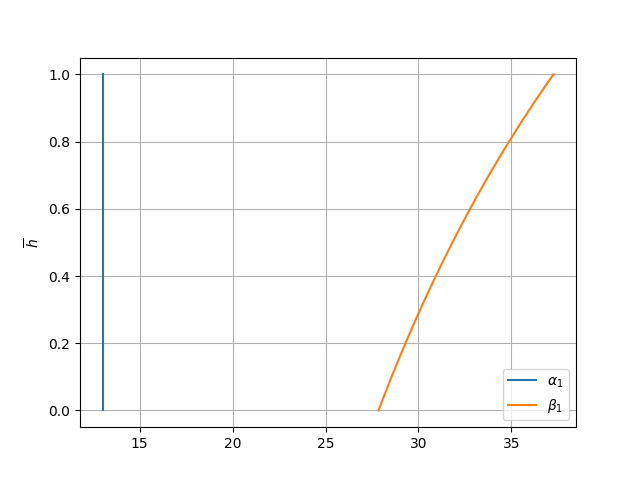
\includegraphics[scale=0.6]{inlet_angle}
		\caption{Углы на входе в лопатки турбины}
	\end{figure}

	\begin{figure}[H]
		\centering
		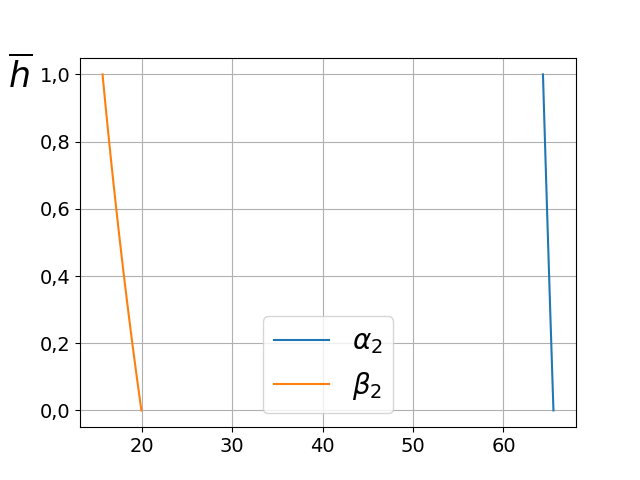
\includegraphics[scale=0.6]{outlet_angle}
		\caption{Углы на выходе из лопаток турбины}
	\end{figure}

%Ниже представлены профили лопаток статора и ротора на трех радиусах
%    \begin{figure}
%        \centering
%        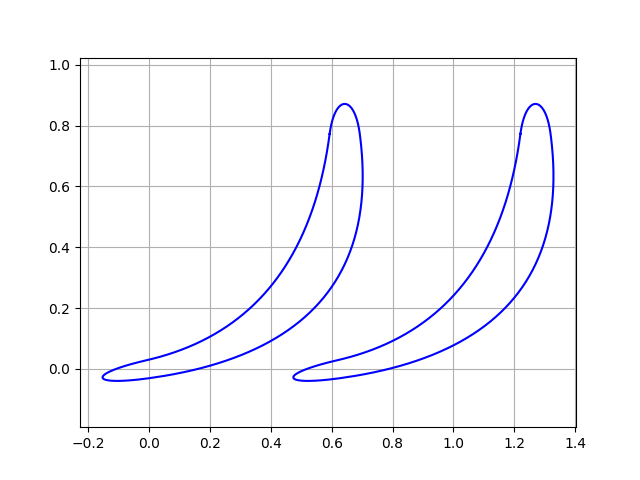
\includegraphics[scale=0.6]{stator_root}
%        \caption{Профиль статора на втулке}
%    \end{figure}
%
%    \begin{figure}
%        \centering
%        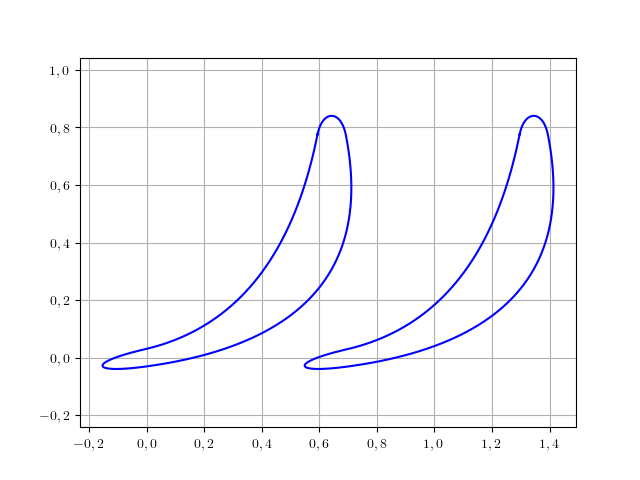
\includegraphics[scale=0.6]{stator_mid}
%        \caption{Профиль статора на среднем радиусе}
%    \end{figure}
%
%    \begin{figure}
%        \centering
%        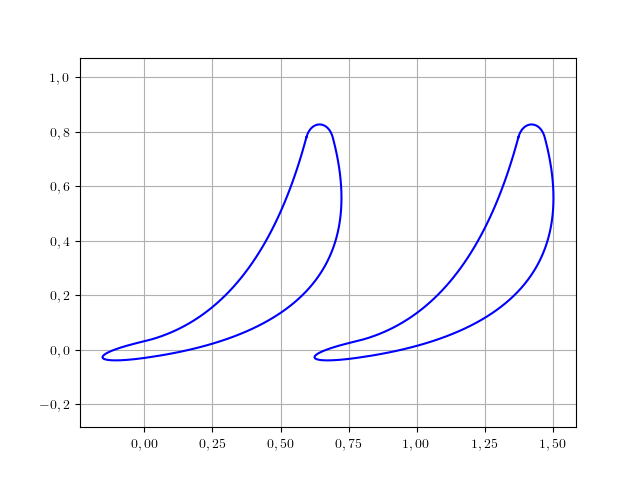
\includegraphics[scale=0.6]{stator_top}
%        \caption{Профиль статора на периферии}
%    \end{figure}
%
%    \begin{figure}
%        \centering
%        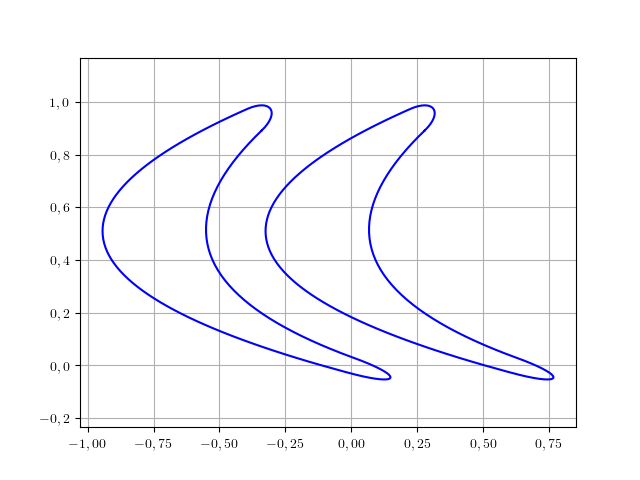
\includegraphics[scale=0.6]{rotor_root}
%        \caption{Профиль ротора на втулке}
%    \end{figure}
%
%    \begin{figure}
%        \centering
%        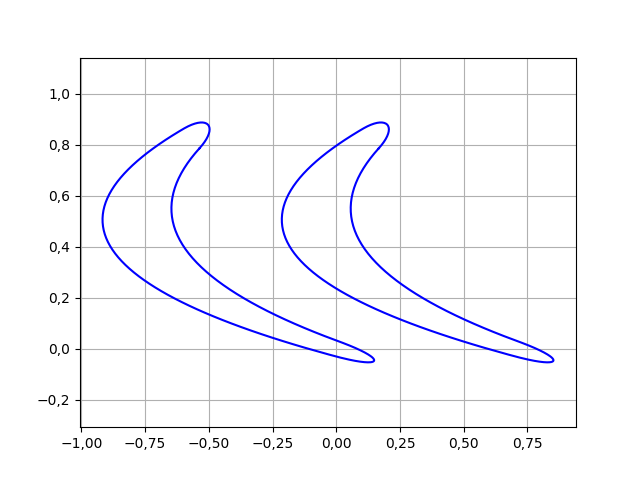
\includegraphics[scale=0.6]{rotor_mid}
%        \caption{Профиль ротора на среднем радиусе}
%    \end{figure}
%
%    \begin{figure}
%        \centering
%        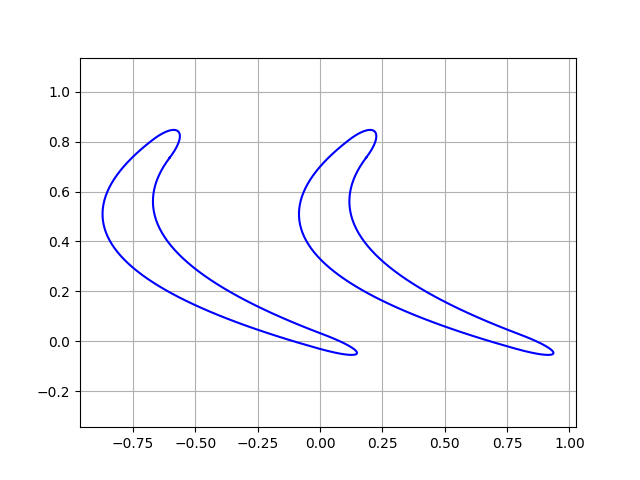
\includegraphics[scale=0.6]{rotor_top}
%        \caption{Профиль ротора на периферии}
%    \end{figure}

    \section{Научно-исследовательская часть}
    \subsection{Сравнительный анализ схем приводов газоперекачивающих агрегатов} % (fold)
\label{sub:сравнительный_анализ_схем_приводов_газоперекачивающих_агрегатов}

\subsubsection{Обзор существующих схем}
Одной из особенностей эксплуатации газотурбинных установок (ГТУ) в качестве привода ГПА является практически постоянная работа установки на режимах частичной мощности [1]. В связи с этим на этапе вариантного проектирования привода ГПА необходимо проводить сравнительную оценку рассматриваемых вариантов в широком диапазоне рабочих мощностей.

В данной работе проводится анализ эффективности работы газотурбинных двигателей различных схем в диапазоне мощностей 30-100\% номинальной мощности и дается оценка эффективности использования ГТУ таких схем в качестве приводов ГПА.

Газотурбинные установки ГПА могут быть разделены на изначально стационарные и конвертированные из авиационных и судовых двигателей.

Все стационарные установки, за исключением ГТ-700-4 и ГТК-25, двухвальные (ГТ-700-4 – одновальная, ГТК-25 - трехвальная). Камеры сгорания стационарных ГТУ индивидуальные, находятся вне корпусов турбин и представляют собой либо одну камеру цилиндрической формы, установленную вертикально или горизонтально, либо несколько секционных камер малого объема, равномерно расположенных по периметру ТВД (ГТН-16 и ГТН-25) [2].

Газотурбинные установки на базе авиационных двигателей являются продуктом конвертирования авиационных турбин. Перед установкой авиационных двигателей на ГПА они переводятся с жидкого топлива на газовое.

Для транспорта используются главным образом двигатели авиалайнеров Ту 114 и Ту 154, НК-12МВ и НК-8-2У с маркировкой после конвертации НК-12СТ и НК-16СТ – мощностью соответственно 6,3 МВт и 16 МВт. Первый из приведенных двигателей входит в состав газоперекачивающего агрегата ГПА-Ц-6,3, а второй – агрегата ГПА-Ц-16 [2].

Отличительными особенностями ГТУ с авиационными двигателями является наличие у них встроенных в корпуса турбин камер сгорания кольцевой формы и большее количество валов по сравнению со стационарными ГТУ (два у ГПА-Ц-6,3 и три у ГПА-Ц-16) [2].

В большинстве такие ГТУ имеют два компрессора и три последовательно расположенные газовые турбины: турбина высокого давления (ТВД), турбина среднего давления (ТСД) и турбина низкого давления (ТНД) – силовая турбина, находящаяся на одном валу с нагнетателем газа. Компрессор первой ступени сжатия приводится во вращение от турбины среднего  давления, компрессор второй ступени сжатия – от турбины высокого давления. Конструктивно вал компрессора первой ступени сжатия и турбины среднего давления   располагается внутри вала, соединяющего компрессор второй ступени сжатия и турбину высокого давления.  Компрессоры первой и второй ступени сжатия  работают на различных частотах вращения. Газотурбинные установки подобных схем позволяют получить высокие соотношения давлений сжатия в цикле – на уровне 16-20, что в сочетании с относительно высокими температурами газов перед ТВД в авиационных ГТУ () позволяет получать КПД установки на уровне 34-35\% и даже выше [2].

Желание получить в газотурбинных установках большую удельную мощность и высокий КПД, привело к разработке и созданию установок с несколькими ступенями сжатия воздуха в осевых компрессорах и его промежуточным охлаждением в процессе сжатия между компрессорами, несколькими ступенями подогрева рабочего тела между газовыми турбинами в процессе его расширения и с регенерацией теплоты отходящих газов. Комплексное использование теплотехнических мероприятий: промежуточное охлаждение воздуха в процессе его сжатия, регенеративный подогрев воздуха после компрессоров и промежуточный подвод тепла в процессе расширения, дают наибольший эффект как на пути повышения КПД установки (который может достигать величины порядка 40-45\% [1]), так  и удельной мощности ГТУ.

Однако, трудность освоения и использования сложных схем ГТУ,  низкие показатели теплообменных аппаратов,  отсутствие мобильности при эксплуатации установок приводят к тому, такие установки целесообразны к использованию только в системах большой энергетики [2].

В данной работе проводится анализ установок следующих схем:
\begin{itemize}
	\item Двухвальная установка со свободной турбиной.
	\item Двухвальная установка со свободной турбиной и регенератором.
	\item Трехвальная установка со свободной турбиной.
\end{itemize}

\subsubsection{Расчетная модель}

В данной работе моделирование ГТУ производится на уровне модели первого уровня, то есть установка разбивается на узлы, взаимодействие между которыми описывается с помощью уравнений, отображающих балансы расходов, энергий и импульсов.

В составе ГТУ можно выделить следующие узлы:
\begin{itemize}
	\item Компрессор;
	\item Турбина;
	\item Камера сгорания;
	\item Регенератор;
	\item Узел потери давления (таким узлом моделируются фильтры, трубопроводы и пр.);
	\item Трансмиссии (с их помощью в модель вводятся механические потери передачи мощности от турбины к компрессору);
	\item Узлы нагрузки, моделирующие внешних потребителей мощности.
\end{itemize}

Узлы компрессоров, турбин, камер сгорания и регенераторов реализованы в двух вариантах: в варианте, позволяющем проводить завязку двигателя на номинальном режиме работы и варианте, позволяющем рассчитывать параметры двигателя на режимах частичной мощности. Такое разделение сделано для оптимизации времени численного счета, так как схема, составленная только из узлов, предназначенных для расчета двигателя на номинальном режиме, не требует численного решения систем нелинейных уравнений и, следовательно, имеет гораздо меньшую вычислительную сложность.

Расчетные узлы компрессоров, турбин и камер сгорания на номинальном режиме работы были реализованы по методике [3].

Регенератор на номинальном режиме работы задавался своим коэффициентом регенерации , определяемым по следующей формуле:
$$
\sigma = \frac{
T_{г \ вх} - T_{г \ вых}
}{
T_{г \ вх} - T_{х \ вх}
}
$$
где $T_{г \ вх}$, К – температура газа на входе в горячий канал теплообменного аппарата, $T_{г \ вых}$, К – температура газа на выходе из горячего канале теплообменного аппарата, $T_{х \ вх}$, К - температура на входе в холодный канал теплообменного аппарата, $T_{х \ вых}$, К – температура на выходе из холодного канала теплообменного аппарата.

Узел потери давления задавался коэффициентом сохранения полного давления $\sigma$, связывающий входное $p_{вх}$, Па и выходное $p_{вых}$, Па давления на границах узла следующим соотношением:
$$
p_{вых} = \sigma \cdot p_{вх}.
$$
Узлы трансмиссии задавались своими механическими КПД $\eta_м$, связывающими механическую мощность на выходе из узла $N_{вых}$, Вт и на входе в него $N_{вх}$, Вт следующим соотношением:
$$
N_{вых} = N_{вх} \cdot \eta_м.
$$

На режиме частичной мощности узлы компрессоров, турбин и камер сгорания рассчитывались, согласно методике [4]. В качестве характеристик компрессоров использовались обобщенные характеристики из [5]. В качестве характеристик турбин использовались обобщенные соотношения из [6].

Регенератор на режиме частичной мощности рассчитывался по методике [7].

Полезная нагрузка на режиме частичной мощности задавалась своей характеристикой в форме:
$$
N_e = N_{e0} \cdot \left( \frac{n}{n_0} \right)^3
$$

где $N_e$, МВт – мощность нагрузки, $N_{e0}$, МВт – мощность нагрузки на номинальной частоте вращения,  $n$б об/мин – частота вращения вала нагрузки, $n_0$б об/мин – номинальная частота вращения вала нагрузки. Такая характеристика нагрузки является характерной для центробежных нагнетателей природного газа [8].

\subsubsection{Условия сравнения установок}

Сравнение установок проводилось в следующих условиях:
\begin{itemize}
	\item Номинальная мощность установок – 16 МВт.
	\item Температура газа в основной камере сгорания – 1450 К.
	\item Для трехвальных установок степени повышения давления в обоих компрессорах равны.
\end{itemize}

Параметры, общие для всех установок, представлены в таблице ~\ref{tab:cycle-comparison}.

\begin{longtable}{|p{7cm}|c|c|c|}
	\caption{Параметры, общие для всех установок}
	\label{tab:cycle-comparison}
	\endfirsthead
	\caption*{\tabcapalign Продолжение таблицы~\thetable}\\[-0.45\onelineskip]
	\hline
	\textbf{Величина} & \textbf{Обозначение} & \textbf{Размерность} & \textbf{Значение} \\ \hline
	\endhead
	\hline
	\textbf{Величина} & \textbf{Обозначение} & \textbf{Размерность} & \textbf{Значение} \\ \hline
	Температура атмосферного воздуха & $T_в$ & К & 288 \\\hline
	Давление атмосферного воздуха & $p_в$ & Па $10^5$ \\\hline
	Температура газа на номинальном режиме & $T_г$ & К & 1450 \\\hline
	Температура топлива & $T_т$ & К & 300 \\\hline
	Калориметрическая температура & $T_0$ К & 300 \\\hline
	Коэффициент сохранения полного давления во входном устройстве & $\sigma_{вх}$ & - & 0,98 \\\hline
	Коэффициент сохранения полного давления во выходном устройстве & $\sigma_{вых}$ & - & 0,93 \\\hline
	Коэффициент сохранения полного давления в основной камере сгорания & $\sigma_{г}$ & - & 0,98 \\\hline
	Полнота сгорания топлива в основной камере сгорания & $\eta_г$ & - & 0,99 \\\hline
	Механические КПД валов & $\eta_м$ & - & 0,99 \\\hline
	Мощность нагрузки на номинальном режиме & $N_e$ & МВт & 16 \\hline
	Частота вращения вала нагрузки на номинальном режиме & $n_0$ & об/мин & 3000 \\\hline
\end{longtable}

На номинальном режиме проводилось исследование зависимости удельной работы $L_e$, Дж/кг, КПД установки $\eta_e$ и расхода воздуха через входное сечение первого компрессора $G_в$, кг/с от степени повышения давления в компрессорах.

Для удобства сравнения на графиках все значения отнесены к максимальным значениям соответствующих параметров, достигающихся на рассматриваемом диапазоне. Относительные параметры определяются следующим образом:
$$
\overline{L_e} = L_e / L_{e \ max},
$$
$$
\overline{\eta_e} = \eta_e / \eta_{e \ max},
$$
$$
\overline{G_в} = G_в / G_{в \ max}.
$$

На режимах частичной мощности исследовались зависимости КПД и расхода воздуха через входное сечение первого компрессора от мощности установки. На графиках этого вида для удобства также представлены зависимости параметров $\overline{\eta_e}$ и $\overline{G_в}$ от параметра $\overline{N_e} = n_e / N_{e \ ном}$, где $N_{e \ ном}$ - номинальная мощность установки (для всех установок $N_{e \ ном} = 16 МВт$).

\subsubsection{Результаты расчетов}
Ниже представленые результаты расчетов различных схем установок для условий сравнения, описанных выше.

Двухвальная безрегенеративная схема преставлена на рис. ~\ref{img:cycle_2n_scheme}.

\begin{figure}[H]
	\centering
	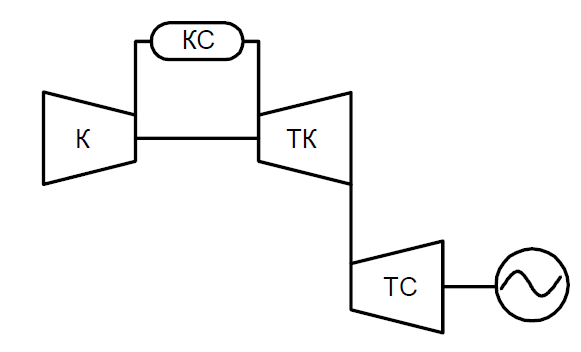
\includegraphics[scale=0.4]{cycle_2n_scheme}
	\caption{Схема двухвальной безрегенеративной установки (К – компрессора, КС – камера сгорания, ТК – турбина компрессора, ТС – силовая турбина)}
	\label{img:cycle_2n_scheme}
\end{figure}

Параметры, характерные для двухавальной безрегенеративной установки, представлены в табл. ~\ref{tab:cycle-2n-parameters}.

\begin{longtable}{|p{7cm}|c|c|c|}
	\caption{Параметры двухвальной безрегенеративной схемы}
	\label{tab:cycle-2n-parameters}
	\endfirsthead
	\caption*{\tabcapalign Продолжение таблицы~\thetable}\\[-0.45\onelineskip]
	\hline
	\textbf{Величина} & \textbf{Обозначение} & \textbf{Размерность} & \textbf{Значение} \\ \hline
	\endhead
	\hline
	\textbf{Величина} & \textbf{Обозначение} & \textbf{Размерность} & \textbf{Значение} \\ \hline
	Адиабатический КПД компрессора & $\eta_к^*$ & - & 0,82 \\ \hline
	КПД тубины компрессора & $\eta_{тк}^*$ & - & 0,90 \\ \hline
	КПД силовой турбины & $\eta_{тс}^*$ & - & 0,92 \\ \hline
	Номинальная частота вращения вала высокого давления & $n_{0 \ вд} $ об/мин & $12 \cdot 10^3$ \\ \hline
\end{longtable}

Параметры цикла двухвальной безрегенеративной установки на номинальном режиме представлены на рис. ~\ref{img:cycle_2n_opt}.

\begin{figure}[H]
	\centering
	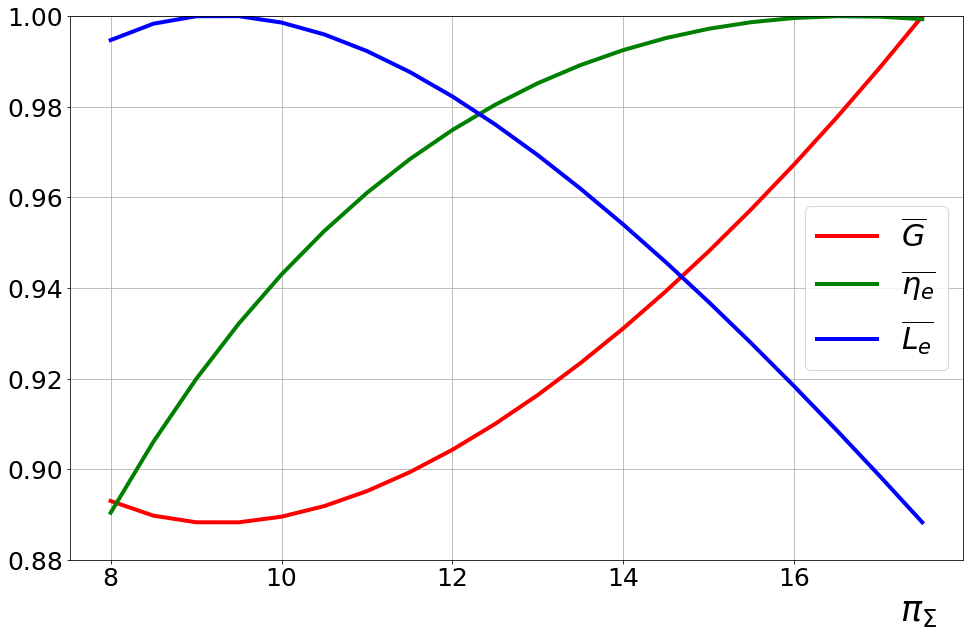
\includegraphics[scale=0.4]{cycle_2n_opt}
	\caption{Параметры цикла двухвальной безрегенеративной установки на номинальном режиме}
	\label{img:cycle_2n_opt}
\end{figure}

В точке, соответствующей максимальному КПД установка имеет параметры, указанные в табл. ~\ref{tab:cycle_2n_max_eta}.

\begin{longtable}{|p{7cm}|c|c|c|}
	\caption{Параметры двухвальной безрегенеративной установки в точке, соответствующей максимальному КПД}
	\label{tab:cycle_2n_max_eta}
	\hline
	\textbf{$\pi_к$} & \textbf{$L_e, \ МДж/кг$} & \textbf{$\eta_e$} & \textbf{$G_в, \ кг/с$} \\ \hline
	16,5 & 0,270 & 0,325 & 59,2 \\ \hline
\end{longtable}


В точке, соответствующей максимальной удельной работе установка имеет параметры, указанные в табл. ~\ref{tab:cycle_2n_max_labour}.
\begin{longtable}{|p{7cm}|c|c|c|}
	\caption{Параметры двухвальной безрегенеративной установки в точке, соответствующей максимальной удельной работе}
	\label{tab:cycle_2n_max_labour}
	\hline
	\textbf{$\pi_к$} & \textbf{$L_e, \ МДж/кг$} & \textbf{$\eta_e$} & \textbf{$G_в, \ кг/с$} \\ \hline
	9,5 & 0,297 & 0,303 & 53,8 \\ \hline
\end{longtable}

В качестве расчетной выбирается точка, соответствующая максимальному КПД.

Параметры двухвальной безрегенеративной схемы представлены на рис. ~\ref{img:cycle_2n_part}.

\begin{figure}[H]
	\centering
	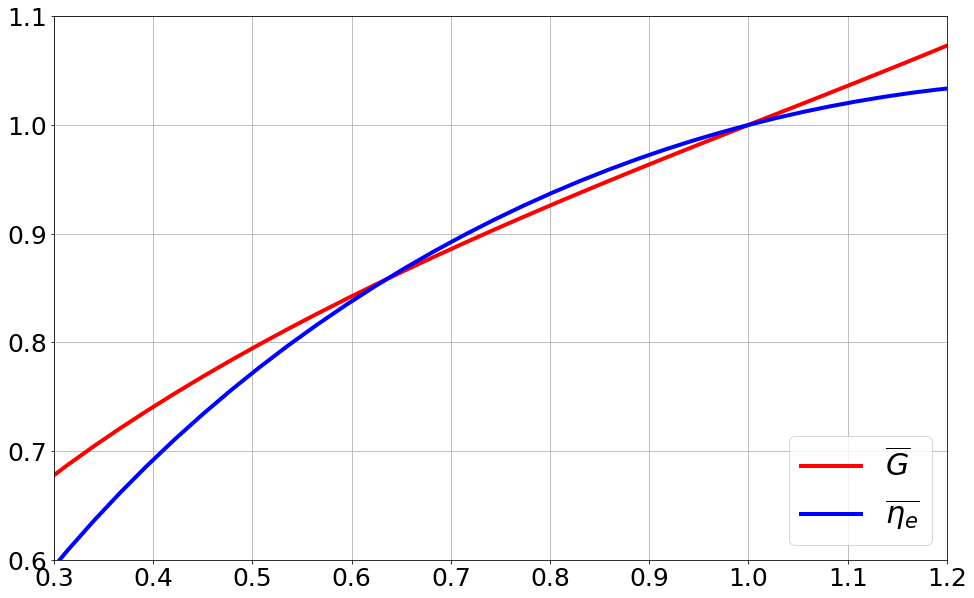
\includegraphics[scale=0.4]{cycle_2n_part}
	\caption{Параметры цикла двухвальной безрегенеративной установки на режимах частичной мощности}
	\label{img:cycle_2n_part}
\end{figure}

Двухвальная регенеративная схема преставлена на рис. ~\ref{img:cycle_2nr_scheme}.

\begin{figure}[H]
	\centering
	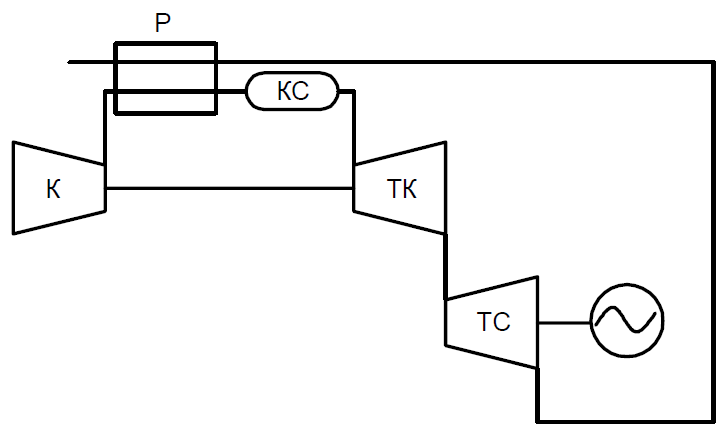
\includegraphics[scale=0.4]{cycle_2nr_scheme}
	\caption{Схема двухвальной регенеративной установки (К – компрессора, КС – камера сгорания, ТК – турбина компрессора, ТС – силовая турбина, Р - регенератор)}
	\label{img:cycle_2nr_scheme}
\end{figure}

Параметры регенеративной двухвальной установки идентичны параметрам установки без регенератора (табл. ~\ref{img:cycle_2n_opt}). Коэффициент регенерации на номинальном режиме $\sigma_р = 0,8$.

Параметры цикла двухвальной безрегенеративной установки на номинальном режиме представлены на рис. ~\ref{img:cycle_2nr_opt}.

\begin{figure}[H]
	\centering
	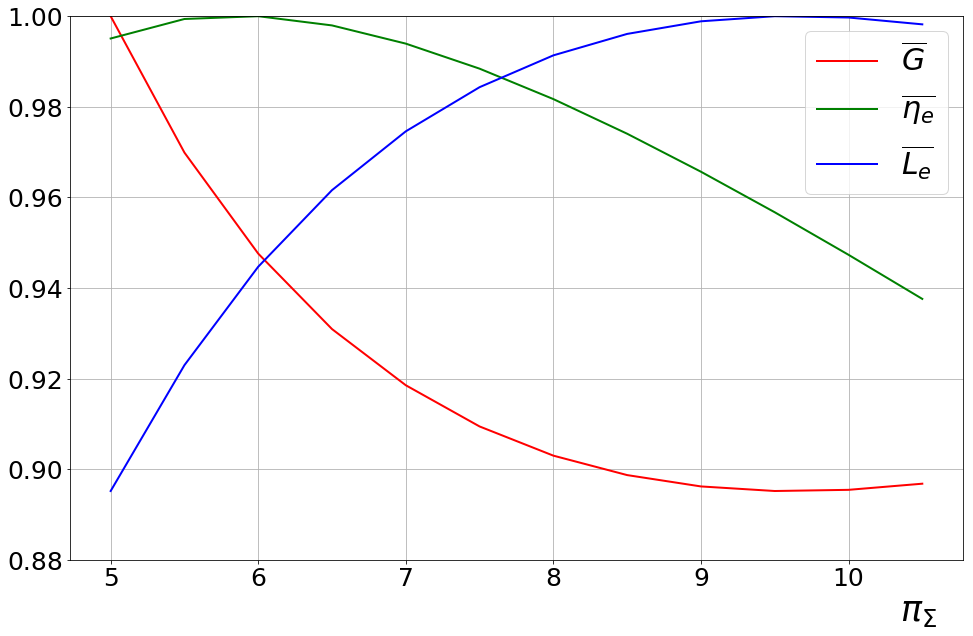
\includegraphics[scale=0.4]{cycle_2nr_opt}
	\caption{Параметры цикла двухвальной регенеративной установки на номинальном режиме}
	\label{img:cycle_2n_opt}
\end{figure}

В точке, соответствующей максимальному КПД установка имеет параметры, указанные в табл. ~\ref{tab:cycle_2nr_max_eta}.

\begin{longtable}{|p{7cm}|c|c|c|}
	\caption{Параметры двухвальной регенеративной установки в точке, соответствующей максимальному КПД}
	\label{tab:cycle_2nr_max_eta}
	\hline
	\textbf{$\pi_к$} & \textbf{$L_e, \ МДж/кг$} & \textbf{$\eta_e$} & \textbf{$G_в, \ кг/с$} \\ \hline
	6,0 & 0,281 & 0,419 & 57,0 \\ \hline
\end{longtable}


В точке, соответствующей максимальной удельной работе установка имеет параметры, указанные в табл. ~\ref{tab:cycle_2n_max_labour}.
\begin{longtable}{|p{7cm}|c|c|c|}
	\caption{Параметры двухвальной регенеративной установки в точке, соответствующей максимальной удельной работе}
	\label{tab:cycle_2nr_max_labour}
	\hline
	\textbf{$\pi_к$} & \textbf{$L_e, \ МДж/кг$} & \textbf{$\eta_e$} & \textbf{$G_в, \ кг/с$} \\ \hline
	9,5 & 0,297 & 0,401 & 53,8 \\ \hline
\end{longtable}

В качестве расчетной выбирается точка, соответствующая максимальному КПД.

Параметры двухвальной регенеративной схемы представлены на рис. ~\ref{img:cycle_2nr_part}.

\begin{figure}[H]
	\centering
	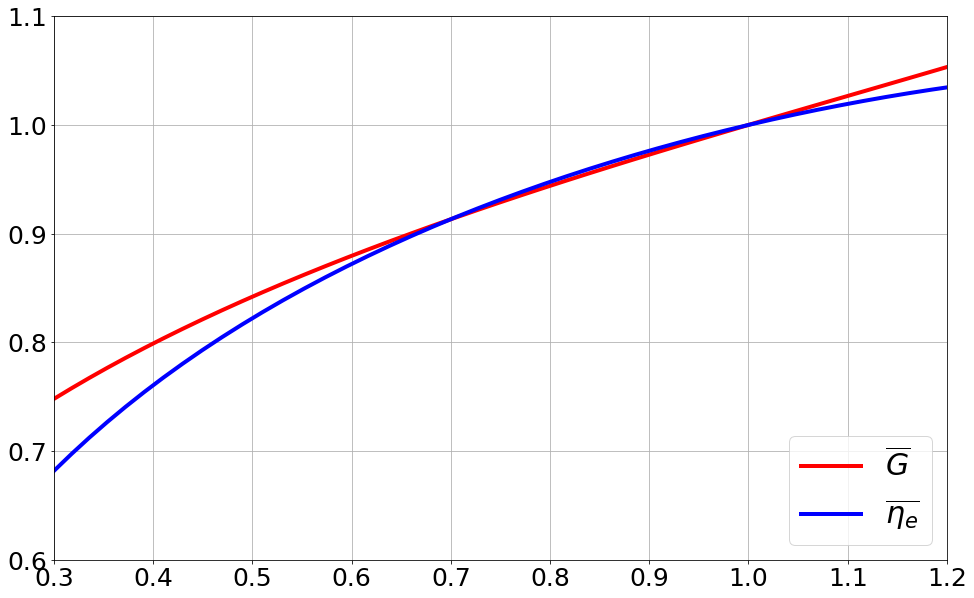
\includegraphics[scale=0.4]{cycle_2nr_part}
	\caption{Параметры цикла двухвальной регенеративной установки на режимах частичной мощности}
	\label{img:cycle_2nr_part}
\end{figure}

Трехвальная схема преставлена на рис. ~\ref{img:cycle_3n_scheme}.

\begin{figure}[H]
	\centering
	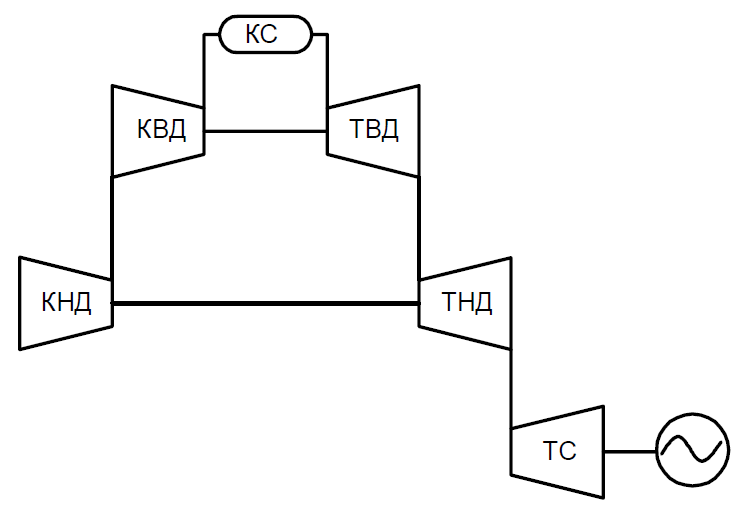
\includegraphics[scale=0.4]{cycle_3n_scheme}
	\caption{Схема трехвальной установки (КНД – компрессор низкого давления, КВД – компрессор высокого давления, КС – камера сгорания, ТВД – турбина высокого давленя, ТНД – турбина низкого давления, ТС – силовая тубина)}
	\label{img:cycle_3n_scheme}
\end{figure}

Параметры, характерные для трехвальной установки, представлены в табл. ~\ref{tab:cycle-3n-parameters}.

\begin{longtable}{|p{7cm}|c|c|c|}
	\caption{Параметры трехвальной схемы}
	\label{tab:cycle-3n-parameters}
	\endfirsthead
	\caption*{\tabcapalign Продолжение таблицы~\thetable}\\[-0.45\onelineskip]
	\hline
	\textbf{Величина} & \textbf{Обозначение} & \textbf{Размерность} & \textbf{Значение} \\ \hline
	\endhead
	\hline
	\textbf{Величина} & \textbf{Обозначение} & \textbf{Размерность} & \textbf{Значение} \\ \hline
	Адиабатический КПД компрессора низкого давления & $\eta_{кнд}^*$ & - & 0,84 \\ \hline
	Адиабатический КПД компрессора высокого давления & $\eta_{квд}^*$ & - & 0,86 \\ \hline
	КПД турбины низкого давления & $\eta_{тнд}^*$ & - & 0,90 \\ \hline
	КПД турбины высокого давления & $\eta_{твд}^*$ & - & 0,88 \\ \hline
	КПД силовой турбины & $\eta_{тс}^*$ & - & 0,92 \\ \hline
	Номинальная частота вращения вала высокого давления & $n_{0вд}$ & об/мин & 12000 \\ \hline
	Номинальная частота вращения вала низкого давления & $n_{0нд}$ & об/мин & 9500 \\ \hline
\end{longtable}

Параметры цикла трехвальной установки на номинальном режиме представлены на рис. ~\ref{img:cycle_3n_opt}.

\begin{figure}[H]
	\centering
	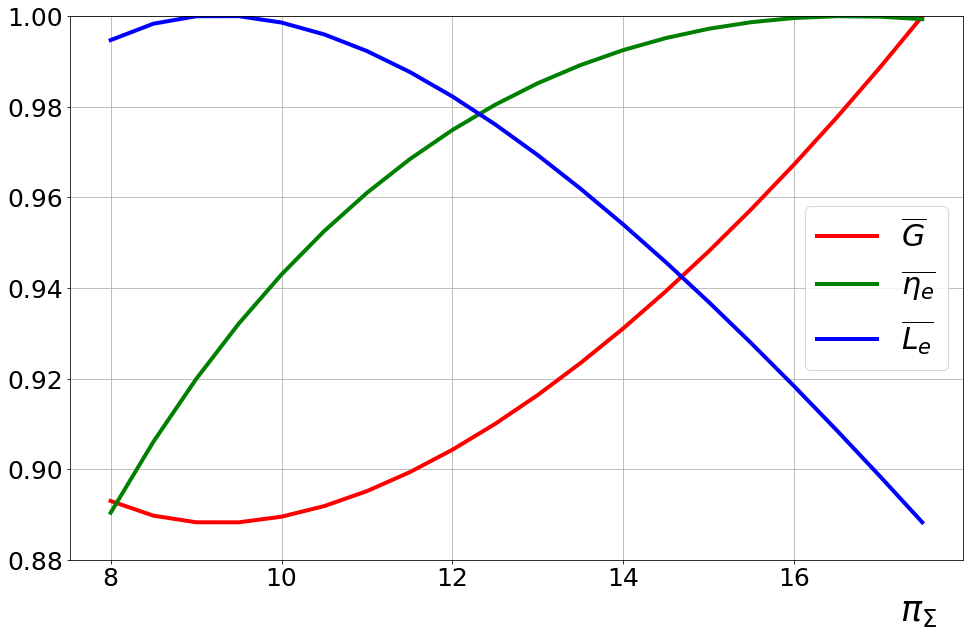
\includegraphics[scale=0.4]{cycle_2n_opt}
	\caption{Параметры цикла двухвальной безрегенеративной установки на номинальном режиме}
	\label{img:cycle_2n_opt}
\end{figure}

В точке, соответствующей максимальному КПД установка имеет параметры, указанные в табл. ~\ref{tab:cycle_3n_max_eta}.

\begin{longtable}{|p{7cm}|c|c|c|}
	\caption{Параметры трехвальной установки в точке, соответствующей максимальному КПД}
	\label{tab:cycle_3n_max_eta}
	\hline
	\textbf{$\pi_к$} & \textbf{$L_e, \ МДж/кг$} & \textbf{$\eta_e$} & \textbf{$G_в, \ кг/с$} \\ \hline
	22,0 & 0,279 & 0,392 & 57,4 \\ \hline
\end{longtable}


В точке, соответствующей максимальной удельной работе установка имеет параметры, указанные в табл. ~\ref{tab:cycle_3n_max_labour}.
\begin{longtable}{|p{7cm}|c|c|c|}
	\caption{Параметры трехвальной установки в точке, соответствующей максимальной удельной работе}
	\label{tab:cycle_3n_max_labour}
	\hline
	\textbf{$\pi_к$} & \textbf{$L_e, \ МДж/кг$} & \textbf{$\eta_e$} & \textbf{$G_в, \ кг/с$} \\ \hline
	11,0 & 0,315 & 0,321 & 50,8 \\ \hline
\end{longtable}

В качестве расчетной выбирается точка, соответствующая максимальному КПД.

Параметры двухвальной безрегенеративной схемы представлены на рис. ~\ref{img:cycle_3n_part}.

\begin{figure}[H]
	\centering
	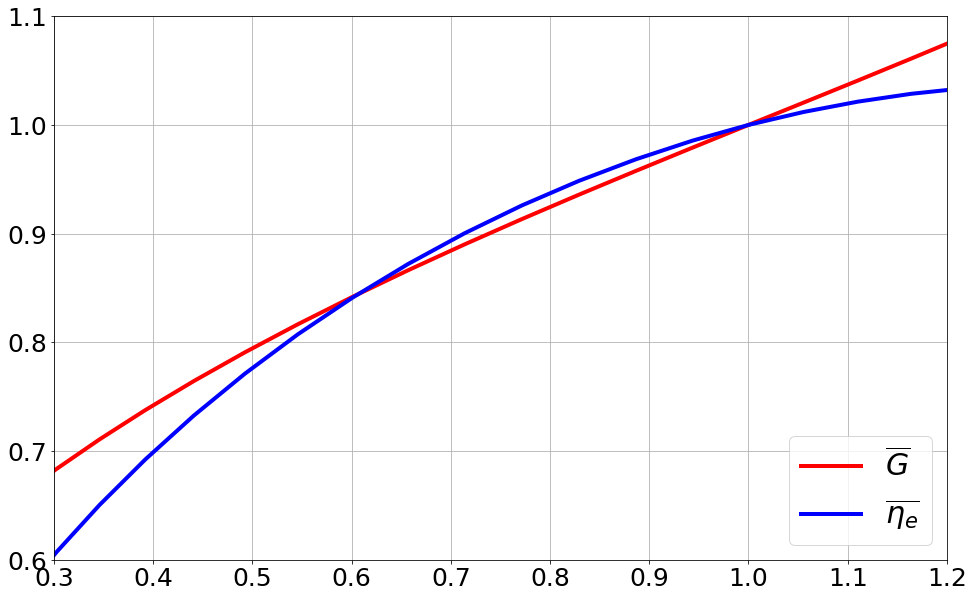
\includegraphics[scale=0.4]{cycle_3n_part}
	\caption{Параметры цикла трехвальной установки на режимах частичной мощности}
	\label{img:cycle_3n_part}
\end{figure}

\subsubsection{Анализ полученных данных}
Сравним КПД установок на режимах частичной мощности. Для этого построим зависимости на одном графике зависимости КПД от мощности установки (рис. ~\ref{img:cycle_eta_comparison}). Для удобства отнесем все значения к максимальному КПД из всех установок (номинальному КПД двухвальной регенеративной схемы).

\begin{figure}[H]
	\centering
	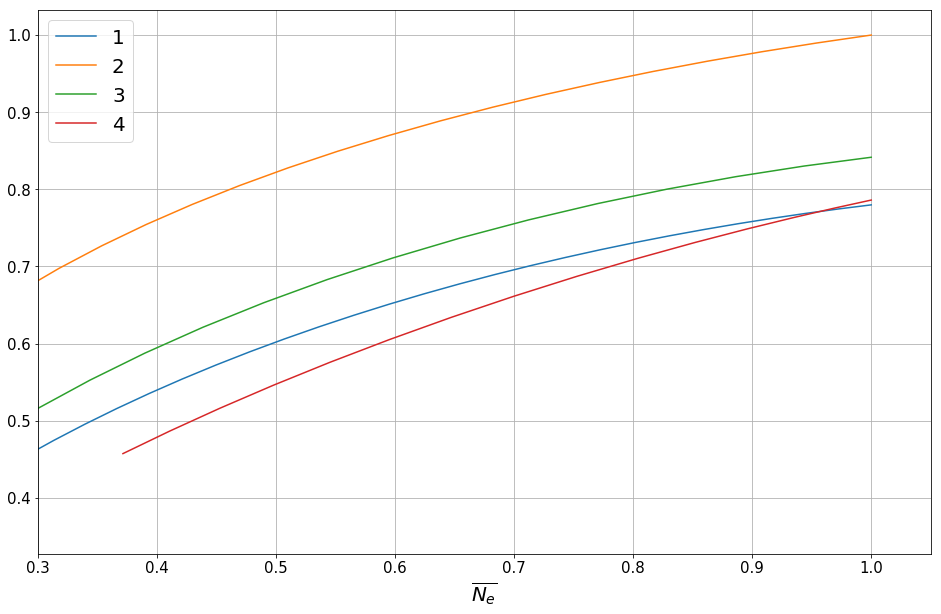
\includegraphics[scale=0.4]{cycle_eta_comparison}
	\caption{Сравнение абсолютных КПД установок (1 – двухвальная безрегенеративная схема, 2 – двухвальная регенеративная схема, 3 – трехвальная схема)}
	\label{img:cycle_eta_comparison}
\end{figure}

Из полученного графика видно, что на всех режимах наиболее эффективным с точки зрения использования топлива является регенеративная схема. Также достоинством данной схемы является снижение удельной работы при снижении мощности установки. Благодаря этому расход в регенеративной схеме по мере уменьшения мощности падает медленнее, чем в безрегенеративной. Однако применение данной схемы приводит к существенному утяжелению установки и увеличению ее инертности, что крайне нежелательно в случае привода ГПА.

Переход от двухвальной к трехвальной схеме приводит к увеличению КПД установки, за счет увеличения КПД компрессоров и турбин, которые работают при меньшей нагрузке, чем в случае двухвальной схемы. Однако область более высокого КПД сдвигается вправо по суммарной степени повышения давления в установке. В связи с этим предполагаемый рост КПД может быть нивелирован увеличением потерь в радиальном зазоре лопаток КВД и ТВД.

Тем не менее, разработка приводов ГПА мощностью 16 МВт по данной схеме вполне оправдана, так как в этом случае размеры лопаток ТВД и КВД оказываются не меньше нескольких десятков миллиметров.


\subsubsection{Заключение}

В данной исследовании был проведен сравнительный анализ трех схем привода ГПА на 16 МВт: двухвальная безрегенеративная схема, двухвальная регенеративная схема, трехвальная схема. Были рассмотрены термодинамические параметры этих схем как на номинальном режиме, так и на режимах частичной мощности.

Использование регенеративной двухвальной схемы позволило сильно увеличить КПД установки по отношению к безрегенеративному варианту (с 0.325 до 0.419) при уменьшении степени сжатия (с 16.5 до 9.5), что положительно сказывается на КПД лопаточных машин высокого давления. Однако применение регенеративной схемы связано с серьезным увеличением капитальных затрат на производство установки. В связи с этим использование данной схемы в качестве привода ГПА кажется нецелесообразным.

Было показано, что переход к трехвальной схеме позволяет повысить КПД установки (c 0.325 до 0.351) при слабом снижении расхода воздуха (c 59.2 до 57.4 кг/с).

    \subsection{Расчет расхода охлаждающего воздуха}

Исходные данные для расчета количества охлаждаемого воздуха представлены в табл. ~\ref{cool1:cool1_inlet}.
Расчет проведен по методике ~\cite{ivanov}.
\begin{longtable}{|p{7cm}|c|c|c|}
	\caption{Исходные данные расхода охлаждающего воздуха}
	\label{cool1:cool1_inlet}
	\endfirsthead
	\caption*{\tabcapalign Продолжение таблицы~\thetable}\\[-0.45\onelineskip]
	\hline
	\textbf{Величина} & \textbf{Обозначение} & \textbf{Размерность} & \textbf{Значение} \\ \hline
	\endhead
	\hline
	\textbf{Величина} & \textbf{Обозначение} & \textbf{Размерность} & \textbf{Значение} \\ \hline
	Температура газа & $T_г$ & К & $1450,0$ \\ \hline
	Начальная температура охлаждающего воздуха & $\theta_0$ & К & $500,0$ \\ \hline
	Длина лопатки & $l$ & м & $58,1 \cdot 10^{-3}$ \\ \hline
	Осевая проекция хорды & $b_a$ & м & $40,0 \cdot 10^{-3}$ \\ \hline
	Поверхность лопатки, соприкасающаяся с газом & $f$ & $м^2$ & $5,4 \cdot 10^{-3}$ \\ \hline
	Периметр профиля & $u$ & $м$ & $93,2 \cdot 10^{-3}$ \\ \hline
	Толщина стенки & $\Delta$ & $м$ & $1,0 \cdot 10^{-3}$ \\ \hline
	Средняя температура наружной поверхности лопатки & $T_{ст}$ & $К$ & $1000,0$ \\ \hline
	Плотность газа & $\rho_г$ & $кг/м^3$ & $4,28$ \\ \hline
	Осевая скорость & $c_a$ & $м/с$ & $110,8$ \\ \hline
\end{longtable}

В качестве материала лопатки принимается сплав ЖС30, выдерживающий при данном уровне температур 250 МПа в течение 10000 ч
~\cite{js_36_properties}.
Данный уровень напряжений заведомо существенно выше напряжений, действующих в короткой двухопорной лопатке, нагруженной
только газодинамическими силами.

 \begin{enumerate}
 	\item Определим число $Re$ для газа ($\mu_г = 52,12 \cdot 10^{-6} Па \cdot с$):
 		$$
 			Re_г = \frac{
 				\rho_г \cdot c_a \cdot b_a
 			}{
 				\mu_г
 			} = \frac{
 				4,28 \cdot 110,8 \cdot 40,0 \cdot 10^{-3}
 			}{
 				52,12 \cdot 10^{-6} 
 			} = 364 \cdot 10^3
 		$$
 	\item Определим число $Nu$ для газа:
 		$$
 			Nu = A \cdot Re_г^{0.68} = 
 			0,079 \cdot \left(
 				364 \cdot 10^3
			\right)^{0.68} = 478
 		$$
 	\item Определим средний коэффициент теплоотдачи от газа к лопатке:
 		$$
 			\alpha_г = Nu \frac{\lambda_г}{b_a} = 
 			478 \cdot \frac{
 				92,9 \cdot 10^{-3}
 			}{
 				40,0 \cdot 10^{-3}
 			} = 1110,5 \/\ Вт / \left( м^2 \cdot К \right)
 		$$
 	\item Определим тепловой поток в сопловую лопатку:
 		$$
 			Q_л = \alpha_г u l \left( T_г - T_{ст} \right) = 
		$$
		$$
 			=1110,5 \cdot 
 			93,2 \cdot 10^{-3} \cdot 
 			58,1 \cdot 10^{-3} \cdot 
 			\left( 
 				1450,0 - 1000 
			\right) = 2,7 \cdot 10^3 \/\ Вт 
 		$$
 	\item Определим падение температуры в тенке лопатки:
 		$$
 			\Delta T_{ст} = \frac{
 				Q_л \cdot \Delta
 			}{
 				f \cdot \lambda_м
 			} = \frac{
 				2,7 \cdot 10^3 \cdot 1,0 \cdot 10^{-3}
 			}{
 				5,4 \cdot 10^{-3} \cdot 20,0
 			} = 25,0 \/\ К 
 		$$
 		($
 			\lambda_м = 20,0 \/\ Вт / \left( м \cdot К\right)
 		$ для ЖС30 при $
 			T_{ср} = T_{ст} - \frac{\Delta T_{ст}}{2} = 1000,0 - \frac{25,0}{2} = 987,5 \/\ К
 		$)
 	\item Определим температуру внутренней поверхности стенки лопатки:
 		$$
 			T_{вн} = T_{ст} - \Delta T_{ст} = 1000,0 - 25,0 = 975,0 К
 		$$
 	\item Задаваясь рядом значений расходов охлаждающего воздуха, определим зависимость зазора в лопатке $\delta$ от расхода охлаждающего воздуха:
 		$$
 			\delta = \varepsilon G_в^{0.8} \left( 
 				D - \frac{
 					f
 				}{
 					7200 \cdot G_в \cdot c_p
 				}
 			\right),
 		$$
 		где 
		$$
			D = \frac{
				1
			}{
				\alpha_г
			} \cdot \frac {
				T_г - \theta_0
			}{
				T_г - T_{ст}
			} - \frac{
				1
			}{
				\alpha_г
			} - \frac{
				\Delta
			}{
				\lambda_м
			};
		$$
		$$
			\epsilon = 0.01 \cdot \lambda \left( 
				\frac{
					1
				}{
					l \mu
				}
			\right)^{0.8}
		$$

 	Результаты расчета расхода охлаждующего воздуха приведены в таблице ~\ref{cool1:mass_rate_result}.
		\begin{center}
			\begin{longtable}{|c|c|c|c|c|}
				\caption{Результаты расчета расхода охлаждающего воздуха} \label{cool1:mass_rate_result}
				\endfirsthead
				\caption*{\tabcapalign Продолжение таблицы~\thetable}\\[-0.45\onelineskip]
				\hline
				\textbf{№} &
				\textbf{$G_в, \/\ кг/c$} &
				\textbf{$D$} &
				\textbf{$\epsilon$} &
				\textbf{$\delta$} \\\hline
				\endhead
				\hline
				\textbf{№} &
				\textbf{$G_в, \/\ кг/c$} &
				\textbf{$D$} &
				\textbf{$\epsilon$} &
				\textbf{$\delta$} \\\hline
				
					1 & 
					$0,01$ & 
					$0,951 \cdot 10^{-3}$ & 
					$17,90$ & 
					$0,3 \cdot 10^-3$ 
					\\\hline
				
					2 & 
					$0,02$ & 
					$0,951 \cdot 10^{-3}$ & 
					$17,90$ & 
					$0,6 \cdot 10^-3$ 
					\\\hline
				
					3 & 
					$0,03$ & 
					$0,951 \cdot 10^{-3}$ & 
					$17,90$ & 
					$0,9 \cdot 10^-3$ 
					\\\hline
				
					4 & 
					$0,04$ & 
					$0,951 \cdot 10^{-3}$ & 
					$17,90$ & 
					$1,2 \cdot 10^-3$ 
					\\\hline
				
					5 & 
					$0,05$ & 
					$0,951 \cdot 10^{-3}$ & 
					$17,90$ & 
					$1,5 \cdot 10^-3$ 
					\\\hline
				
					6 & 
					$0,06$ & 
					$0,951 \cdot 10^{-3}$ & 
					$17,90$ & 
					$1,7 \cdot 10^-3$ 
					\\\hline
				
					7 & 
					$0,07$ & 
					$0,951 \cdot 10^{-3}$ & 
					$17,90$ & 
					$1,9 \cdot 10^-3$ 
					\\\hline
				
					8 & 
					$0,08$ & 
					$0,951 \cdot 10^{-3}$ & 
					$17,90$ & 
					$2,2 \cdot 10^-3$ 
					\\\hline
				
					9 & 
					$0,09$ & 
					$0,951 \cdot 10^{-3}$ & 
					$17,90$ & 
					$2,4 \cdot 10^-3$ 
					\\\hline
				
					10 & 
					$0,10$ & 
					$0,951 \cdot 10^{-3}$ & 
					$17,90$ & 
					$2,6 \cdot 10^-3$ 
					\\\hline
				
			\end{longtable}
		\end{center}

 \end{enumerate}
    \section{Расчет профиля температур}

Для расчета профиля температур лопатки принимаем расход воздуха $G_в = 0.053 кг/c$, а величину зазора между дефлектором и
внутренней поверхностью лопатки $\delta = 1 мм$.

При расчете профиля температур лопатки при конвективно-пленочно охлаждении будем пользоваться следующей методикой:
\begin{enumerate}
	\item Зададим распределение приведенной скорости по корыту $\lambda_к \left( \overline{x} \right)$ и спинке $\lambda_с \left( \overline{x} \right)$:
		$$
			\lambda_к \left( \overline{x} \right) = 
			\left\{ 
				1 + 
				\left[ 
					\left( 
						\frac{\lambda_1}{\lambda_0}
					\right)^{0.5}
				\right]\overline{x}
			\right\}^{2} \lambda_0, \/\ \overline{x} = \frac{x}{l_к}
		$$
		$$
			\lambda_с \left( \overline{x} \right) = 
			\left\{ 
				1 + 
				\left[ 
					\left( 
						\frac{\lambda_1}{\lambda_0}
					\right)^{4}
				\right]\overline{x}
			\right\}^{0.25}\lambda_0, \/\ \overline{x} = \frac{x}{l_с}
		,$$
		где $l_к$ - длина профиля со стороны корыта, $l_с$ - длина профиля со стороны спинки, $\lambda_0$ - приведенная скорость на входе в лопаточный венец, $\lambda_1$ - приведенная скорость на выходе из лопаточного венца.

	\item Определим критическую скорость звука $a_{кр}$:
		$$
			a_{кр} = \sqrt{
				\frac{2k_г}{k_г + 1} R_г T_г^*
			}
		$$
	\item Определим скорость газа на корыте $v_к$ и на спинке $v_с$:
		$$
			v_к\left( x \right) = \lambda_к \left( \frac{x}{l_к} \right)
		$$
		$$
			v_c\left( x \right) = \lambda_к \left( \frac{x}{l_c} \right)
		$$
	Дальнейший расчет идентичен для спинки и корыта, поэтому скорость газа будем обозначать как $v_г$.
	\item Определим эквивалентную ширину щели:
		$$
			s = N_{отв} \frac{\pi d_{отв}^2}{4} \cdot \frac{1}{l},
		$$
		где $N_{отв}$ - количество отверстий, $d_{отв}$ - диаметр отверстия, $l$ - высота профильной части лопатки.
	\item Определим скорость газа в точке выдува воздуха:
		$$
			v_{г \/\ отв} = v_г\left( x_{отв} \right),
		$$
		где $x_{отв}$ - криволинейная координата отверстия.
	\item Определим статическую температуру газа в точке выдува воздуха:
		$$
			T_{г \/\ отв} = T_г^* - \frac{v_{г \/\ отв}}{2 c_{p \/\ г}}
		$$
	\item Определим статическое давление газа в точке выдува воздуха:
	 	$$
	 		p_{г \/\ отв} = \frac{p_г^*}{
	 			\left( 
	 				\frac{
	 					T_г^*
	 				}{
	 					T_{г \/\ отв}
	 				}
	 			\right)^\frac{k_г}{k_г - 1}
	 		}
	 	$$
	\item Определим статическую плотность газа в точке выдува воздуха:
	 	$$
	 		\rho_{г \/\ отв} = \frac{
	 			p_{г \/\ отв}
	 		}{
	 			R_г \cdot T_{г \/\ отв}
	 		}
	 	$$
	\item Определим скорость истечения воздуха из отверстия:
	 	$$
	 		v_{в \/\ отв} = \phi_{отв} \sqrt{
	 			\frac{2k_в}{k_в - 1}
	 		} R_в \theta \left( x_{отв} \right) 
	 		\left[ 
	 			1 - 
	 			\left( 
	 				\frac{
	 					p_{г \/\ отв}
	 				}{
	 					p_{в0}^*
	 				}
	 			\right)^\frac{k_в - 1}{k_в}
	 		\right],
	 	$$
	 	где $\phi_{отв}$ - коэффициент скорости, $\theta \left( x_{отв} \right)$ - температура воздуха в точке выдува, $p_{в0}^*$ - давление воздуха.
	\item Определим статическую плотность воздуха на выходе из отверстия:
		$$
			\rho_{в \/\ отв} = \frac{
				p_{г \/\ отв}
			}{
				R_в
				\left[
					\theta \left( x_{отв} \right) - \frac{v_{в \/\ отв}^2}{2c_{p \/\ в}}
				\right]
			}
		$$
	\item Определим плотность торможения воздуха на входе в отверстия:
		$$
			\rho_{в \/\ отв}^* = \frac{p_{в0}^*}{R_в \theta \left( x_{отв} \right) }
		$$
	\item Определим параметр вдува:
		$$
			m = \frac{\rho_{в \/\ отв} v_{в \/\ отв}}{\rho_{г \/\ отв} v_{г \/\ отв}}
		$$
	\item Определим число Рейнольдса по ширине щели:
		$$
			Re_s = \frac{
				\rho_{г \/\ отв} v_{г \/\ отв} s
			}{\mu_г\left( T_{г \/\ отв} \right)}
		$$
	\item Определим температурный фактор:
		$$
			\phi = \theta \left( x_{отв} \right) / T_г^*
		$$
	\item Определим эффективность пленки $\theta_{пл}\left( x \right)$:
		$$
			A\left( x \right) = Re_s^{-0.25} m^{-1.3} \phi^{-1.25}
			\left(
				\frac{
					x - x_{отв}
				}{
					s
				}
			\right)
		$$
		$$
			\theta_{пл}\left( x \right) = \left\{
				\begin{array}{@{}ll@{}}
					1.0, & \text{если}\ 0 < A \leq 3 \\
					\left( \frac{A}{3} \right)^{-0.285}, & \text{если} 3 \leq A < 11 \\
					\left( \frac{A}{7.43} \right)^{-0.95}, & \text{если} A \geq 11 \\
				\end{array}\right.
		$$
	\item Определим темперутуру пленки в случае нескольких рядов отверстий:
		$$
			T_{пл}^*\left( x \right) = T_г^* \cdot \prod_{i = 1}^{x_i \leq x}
				\left[
					\left(
						1 - \theta_{пл \/\ i}
					\right)
				\right] + 
				\sum_{i = 1}^{x_i \leq x} \left[
					\theta_{пл \/\ i}T_в^*\left( x_{отв \/\ j} \right)
					\prod_{j = i + 1}^{x_j \leq x} 
					\left(
						1 - \theta_{пл \/\ j}
					\right)
				\right]
		$$
	\item Определим коэффициент теплоотдачи пленки в случае нескольких рядов отверстий:
		$$
			\alpha_{пл}\left( x \right) = \alpha_{г}
			\prod_{i = 1}^{x_i \leq x} \left[
				1 + \frac{
					2m_i
				}{
					\frac{
						x - x_{отв \/\ i}
					}{s_i}
				}
			\right]
		$$
	\item По формуле истечения из сопла определим расход через ряд отверстий:
		$$
			G_отв = s \cdot l \cdot  \mu_{отв} \sqrt{
				\frac{2k_в}{k_в - 1} p_{в0}^*\rho_{в \/\ отв}^* 
				\left(
					\frac{
						p_{г \/\ отв}
					}{
						p_{в0}^*
					}
				\right)^\frac{2}{k_в}
				\left[
					1 - 
					\left(
						\frac{
							p_{г \/\ отв}
						}{
							p_{в0}^*
						}
					\right)^\frac{k_в - 1}{k_в}
				\right]
			}
		$$
	\item В общем случае зависимость расхода воздуха в зазоре от криволинейной координаты имеет вид:
		$$
			G_в \left( x \right) = G_{в0} - \sum_{i = 1}^{x_i \leq x} G_{отв \/\ i}
		$$

В данном расчете суммарный расход на охлаждение сопловых лопаток принимается равным
$G_0 = 45 \cdot 10^{-3} \/\ кг/c$ на лопатку, что при числе лопаток статора, равном 54, равно 4.89\% от суммарного расхода
воздуха.
В результате расчетов получим значения характерных параметров в отверстиях.

Значения характерных параметров в отверстиях корыта:
\begin{longtable}{|c|c|c|c|c|c|c|c|c|}
	\hline
	\textbf{№} &
	\textbf{$x, \/\ мм$} & 
	\textbf{$s, \/\ 10^{-3} \/\ мм$} &
	\textbf{$\phi_{отв}$} &
	\textbf{$\mu_{отв}$} &
	\textbf{$m$} & 
	\textbf{$\phi$} & 
	\textbf{$G_{отв}, \/\ 10^{-3} \/\ кг/с$} &
	\textbf{$G_{отв} / G_{в0}$} 
	\\ \hline
	
		1 & 
		4.0 & 
		79.5 &
		0.98 &
		0.98 &
		2.08 &
		0.42 &
		5.25 &
		0.131 
		\\\hline
	
		2 & 
		18.0 & 
		62.8 &
		0.98 &
		0.98 &
		1.87 &
		0.54 &
		3.60 &
		0.090 
		\\\hline
	
		3 & 
		30.0 & 
		98.2 &
		0.98 &
		0.98 &
		1.77 &
		0.63 &
		5.18 &
		0.129 
		\\\hline
	
		4 & 
		37.0 & 
		62.8 &
		0.98 &
		0.98 &
		1.76 &
		0.64 &
		3.25 &
		0.081 
		\\\hline
		
\end{longtable}

Значения характерных параметров в отверстиях спинки:
\begin{longtable}{|c|c|c|c|c|c|c|c|c|}
	\hline
	\textbf{№} &
	\textbf{$x, \/\ мм$} & 
	\textbf{$s, \/\ 10^{-3} \/\ мм$} &
	\textbf{$\phi_{отв}$} &
	\textbf{$\mu_{отв}$} &
	\textbf{$m$} & 
	\textbf{$\phi$} & 
	\textbf{$G_{отв}, \/\ 10^{-3} \/\ кг/с$} &
	\textbf{$G_{отв} / G_{в0}$} 
	\\ \hline
	
		1 & 
		7.0 & 
		79.5 &
		0.98 &
		0.98 &
		2.03 &
		0.44 &
		5.12 &
		0.128 
		\\\hline
	
		2 & 
		22.0 & 
		24.5 &
		0.98 &
		0.98 &
		1.87 &
		0.54 &
		1.41 &
		0.035 
		\\\hline
	
		3 & 
		27.0 & 
		24.5 &
		0.98 &
		0.98 &
		1.84 &
		0.57 &
		1.37 &
		0.034 
		\\\hline
	
		4 & 
		32.0 & 
		40.2 &
		0.98 &
		0.98 &
		1.80 &
		0.60 &
		2.18 &
		0.055 
		\\\hline
	
		5 & 
		38.0 & 
		48.1 &
		0.98 &
		0.98 &
		1.76 &
		0.64 &
		2.52 &
		0.063 
		\\\hline
	
		6 & 
		43.0 & 
		79.5 &
		0.98 &
		0.98 &
		1.75 &
		0.66 &
		4.07 &
		0.102 
		\\\hline
		
\end{longtable}


	\item Определим коэффициент теплоотдачи от газа на входной кромке лопатки $\alpha_{г.вх.кр.}$:
		$$
			\alpha_{г.вх.кр.} = 0.74 \frac{
				\lambda_г
			}{
				d_{вх.кр.}
			}\sqrt{
				\frac{
					\rho_г \cdot c_a \cdot d_{вх.кр.}
				}{
					\mu_г
				}
			} =
		$$
		$$
			= 0.74 \frac{
				92.9 \cdot 10^{-3}
			}{
				2.20 \cdot 10^{-3}
			}\sqrt{
				\frac{
					4.3 \cdot 
					110.8 \cdot 
					2.20 \cdot 10^{-3}
				}{
					52.1 \cdot 10^{-6}
				}
			} = 4424.3 \/\ Вт/\left( м^2 \cdot К\right)
		$$
	\item Определим коэффициент теплоотдачи на спинке на расстоянии $\frac{1}{3} b_a$ $\alpha_{г.вых.кр.}$:
		$$
			\alpha_{г.вых.кр.} = 1.5 \alpha_г = 
			1.5 \cdot 1110.5 = 1665.8 Вт/\left( м^2 \cdot К\right)
		$$
	\item Определим коэффициент теплоотдачи на остальной выпуклой части (спинке) $\alpha_{г.сп.}$:
		$$
			\alpha_{г.сп.} = 0.6 \alpha_г = 0.6 \cdot 1110.5 = 666.3 Вт/\left( м^2 \cdot К\right)
		$$
	\item Определим коэффициет теплоотдачи на вогнутой части профиля (корыте) $\alpha_{г.кор.}$:
		$$
			\alpha_{г.кор.} = \alpha_г = 1110.5 = 1110.5 Вт/\left( м^2 \cdot К\right)
		$$
	\item Коэффициент теплоотдачи от стенки к охлаждающему воздуху зависит от его температуры и определяется следующим уравнением $\alpha_{в}$:
		$$
			\alpha_{в} = 0.02 \cdot \frac{
				\lambda_{в}
			}{
				2\delta
			} \left( 
				\frac{
					G_в
				}{
					l
				} \cdot \frac{
					1
				}{
					\mu_{в}
				}
			\right)^{0.8}
		$$

	Распределение коэффициентов теплоотдачи по профилю лопатки показано на рис. 4. Данное распределение является приближенным - дискретным.
	Реальное распределение коэффциентов теплоотдачи является непрерывным. Характер непрерывного распределениея показан на рис. 5.
	\begin{figure}[H]
	    \centering
    	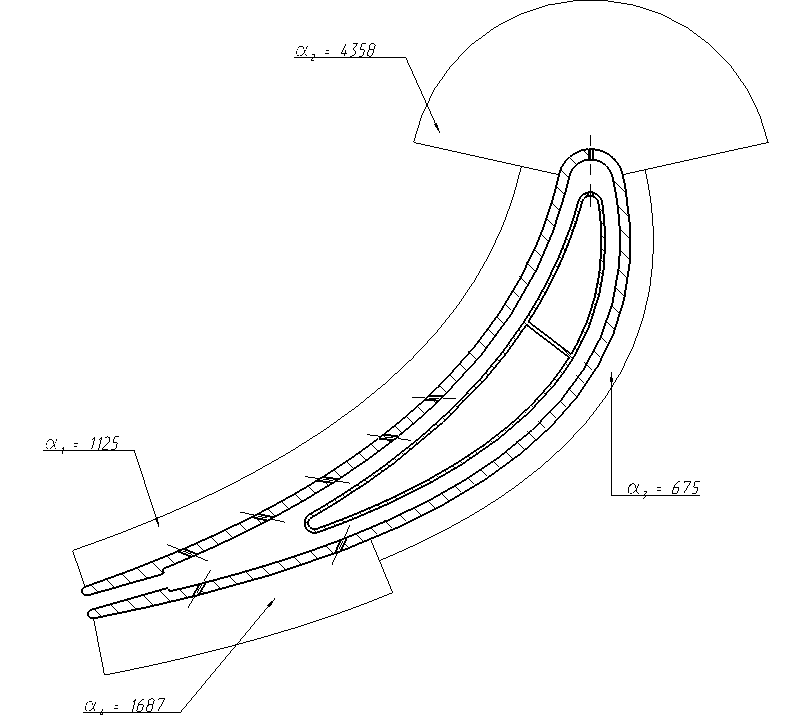
\includegraphics[scale=0.6]{no_spline}
    	\caption{Дискретное распределение коэффициентов теплоотдачи по профилю лопатки}
    \end{figure}

    \begin{figure}[H]
        \centering
        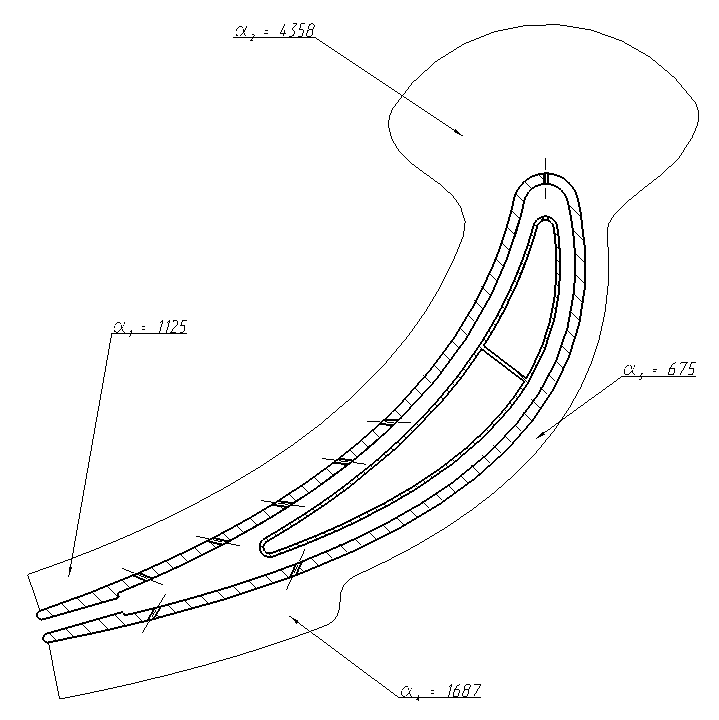
\includegraphics[scale=0.6]{spline}
        \caption{Непрерывное распределение коэффициентов теплоотдачи по профилю лопатки}
    \end{figure}

	\item Уравнение теплообмена между охлаждающим воздухом и газом имеет вид:
		$$
			\frac{d\theta}{dx} = \frac{
				2
			}{
				G_в C_{p \/\ в}
			} \frac{
				k_x
			}{
				\alpha_г
			} \left( 
				T_{пл}^* - \theta
			\right),
		$$
	где $k_x$ - коэффициент теплопередачи, определяемый уравнением
		$$
			k_x = \frac{1}{
				\frac{1}{
					\alpha_{пл}
				} + 
				\frac{1}{
					\alpha_в
				} + 
				\frac{\Delta}{\lambda_м}
			}
		$$
	Численно решая уравнение теплообмена, поулчим распределение параметров по спинке и корыту.
	Распределение параметров газа по спинке:
		\begin{longtable}{|c|c|c|c|c|c|}
		\hline
		\textbf{№} &
		\textbf{$x, \/\ м$} & 
		\textbf{$\alpha_{пл} \/\ Вт/\left(м^2 \cdot К\right)$} & 
		\textbf{$\alpha_в \/\ Вт/\left(м^2 \cdot К\right)$} & 
		\textbf{$\theta_x, \/\ К$} & 
		\textbf{$T_{ст.x}, \/\ К$} 
		\\ \hline
		
			1 & 
			0.000 & 
			4424.3 & 
			1372.6 &
			500.0 & 
			1236.3
			\\\hline
		
			2 & 
			2.705 & 
			666.3 & 
			1417.6 &
			566.0 & 
			862.0
			\\\hline
		
			3 & 
			5.352 & 
			666.3 & 
			1444.7 &
			614.1 & 
			890.7
			\\\hline
		
			4 & 
			7.863 & 
			916.0 & 
			1459.0 &
			643.1 & 
			643.1
			\\\hline
		
			5 & 
			10.253 & 
			732.6 & 
			1462.0 &
			649.4 & 
			711.9
			\\\hline
		
			6 & 
			12.539 & 
			705.2 & 
			1468.9 &
			664.9 & 
			767.6
			\\\hline
		
			7 & 
			14.741 & 
			694.1 & 
			1479.0 &
			688.1 & 
			825.6
			\\\hline
		
			8 & 
			16.882 & 
			688.1 & 
			1489.2 &
			715.0 & 
			866.4
			\\\hline
		
			9 & 
			18.986 & 
			684.3 & 
			1498.5 &
			743.0 & 
			899.4
			\\\hline
		
			10 & 
			21.078 & 
			681.6 & 
			1507.2 &
			771.3 & 
			928.2
			\\\hline
		
			11 & 
			23.184 & 
			732.3 & 
			1511.6 &
			786.3 & 
			835.7
			\\\hline
		
			12 & 
			25.330 & 
			696.8 & 
			1517.0 &
			805.1 & 
			921.1
			\\\hline
		
			13 & 
			27.539 & 
			803.0 & 
			1521.9 &
			824.7 & 
			840.9
			\\\hline
		
			14 & 
			29.834 & 
			705.4 & 
			1525.4 &
			839.1 & 
			931.2
			\\\hline
		
			15 & 
			32.234 & 
			2806.0 & 
			1532.1 &
			863.7 & 
			863.7
			\\\hline
		
			16 & 
			34.757 & 
			1807.5 & 
			1535.4 &
			874.8 & 
			948.1
			\\\hline
		
			17 & 
			37.417 & 
			1754.0 & 
			1545.6 &
			911.1 & 
			1035.4
			\\\hline
		
			18 & 
			40.227 & 
			1863.9 & 
			1549.4 &
			925.4 & 
			958.8
			\\\hline
		
			19 & 
			43.198 & 
			4267.9 & 
			1556.3 &
			951.4 & 
			951.4
			\\\hline
		
			20 & 
			46.339 & 
			1890.8 & 
			1558.3 &
			957.7 & 
			975.3
			\\\hline
		
		\end{longtable}

	Распределение параметров газа по корыту:
		\begin{longtable}{|c|c|c|c|c|c|}
		\hline
		\textbf{№} &
		\textbf{$x, \/\ 10^{-3} м$} & 
		\textbf{$\alpha_{пл} \/\ Вт/\left(м^2 \cdot К\right)$} & 
		\textbf{$\alpha_в \/\ Вт/\left(м^2 \cdot К\right)$} & 
		\textbf{$\theta_x, \/\ К$} & 
		\textbf{$T_{ст.x}, \/\ К$} 
		\\ \hline
		
			1 & 
			0.000 & 
			4424.3 & 
			1372.6 &
			500.0 & 
			1236.3  
			\\\hline
		
			2 & 
			2.577 & 
			1110.5 & 
			1424.7 &
			578.0 & 
			974.8  
			\\\hline
		
			3 & 
			5.198 & 
			1417.0 & 
			1444.2 &
			613.2 & 
			613.2  
			\\\hline
		
			4 & 
			7.731 & 
			1208.9 & 
			1450.8 &
			626.4 & 
			724.9  
			\\\hline
		
			5 & 
			10.179 & 
			1169.9 & 
			1463.9 &
			653.5 & 
			818.5  
			\\\hline
		
			6 & 
			12.550 & 
			1153.5 & 
			1480.5 &
			691.5 & 
			890.2  
			\\\hline
		
			7 & 
			14.848 & 
			1144.4 & 
			1495.0 &
			732.5 & 
			940.2  
			\\\hline
		
			8 & 
			17.081 & 
			1138.6 & 
			1507.7 &
			772.9 & 
			979.8  
			\\\hline
		
			9 & 
			19.256 & 
			1346.4 & 
			1512.6 &
			789.4 & 
			797.3  
			\\\hline
		
			10 & 
			21.380 & 
			1210.1 & 
			1515.3 &
			798.8 & 
			856.7  
			\\\hline
		
			11 & 
			23.463 & 
			1177.9 & 
			1519.9 &
			817.0 & 
			916.0  
			\\\hline
		
			12 & 
			25.514 & 
			1162.8 & 
			1526.5 &
			843.3 & 
			964.8  
			\\\hline
		
			13 & 
			27.541 & 
			1153.8 & 
			1534.8 &
			872.7 & 
			1002.0  
			\\\hline
		
			14 & 
			29.555 & 
			1147.7 & 
			1543.4 &
			902.8 & 
			1033.2  
			\\\hline
		
			15 & 
			31.566 & 
			1396.6 & 
			1545.3 &
			910.0 & 
			910.0  
			\\\hline
		
			16 & 
			33.583 & 
			1250.2 & 
			1546.2 &
			913.3 & 
			932.9  
			\\\hline
		
			17 & 
			35.616 & 
			1207.3 & 
			1549.2 &
			924.8 & 
			956.3  
			\\\hline
		
			18 & 
			37.676 & 
			1574.0 & 
			1551.9 &
			934.8 & 
			934.8  
			\\\hline
		
			19 & 
			39.772 & 
			1266.7 & 
			1553.0 &
			939.2 & 
			950.4  
			\\\hline
		
			20 & 
			41.912 & 
			1216.6 & 
			1557.3 &
			954.5 & 
			974.8  
			\\\hline
			
		\end{longtable}

\end{enumerate}

Распределение температур газа, воздуха и металла по профилю лопатки показано на рис. 6.
\begin{figure}[H]
    \centering
	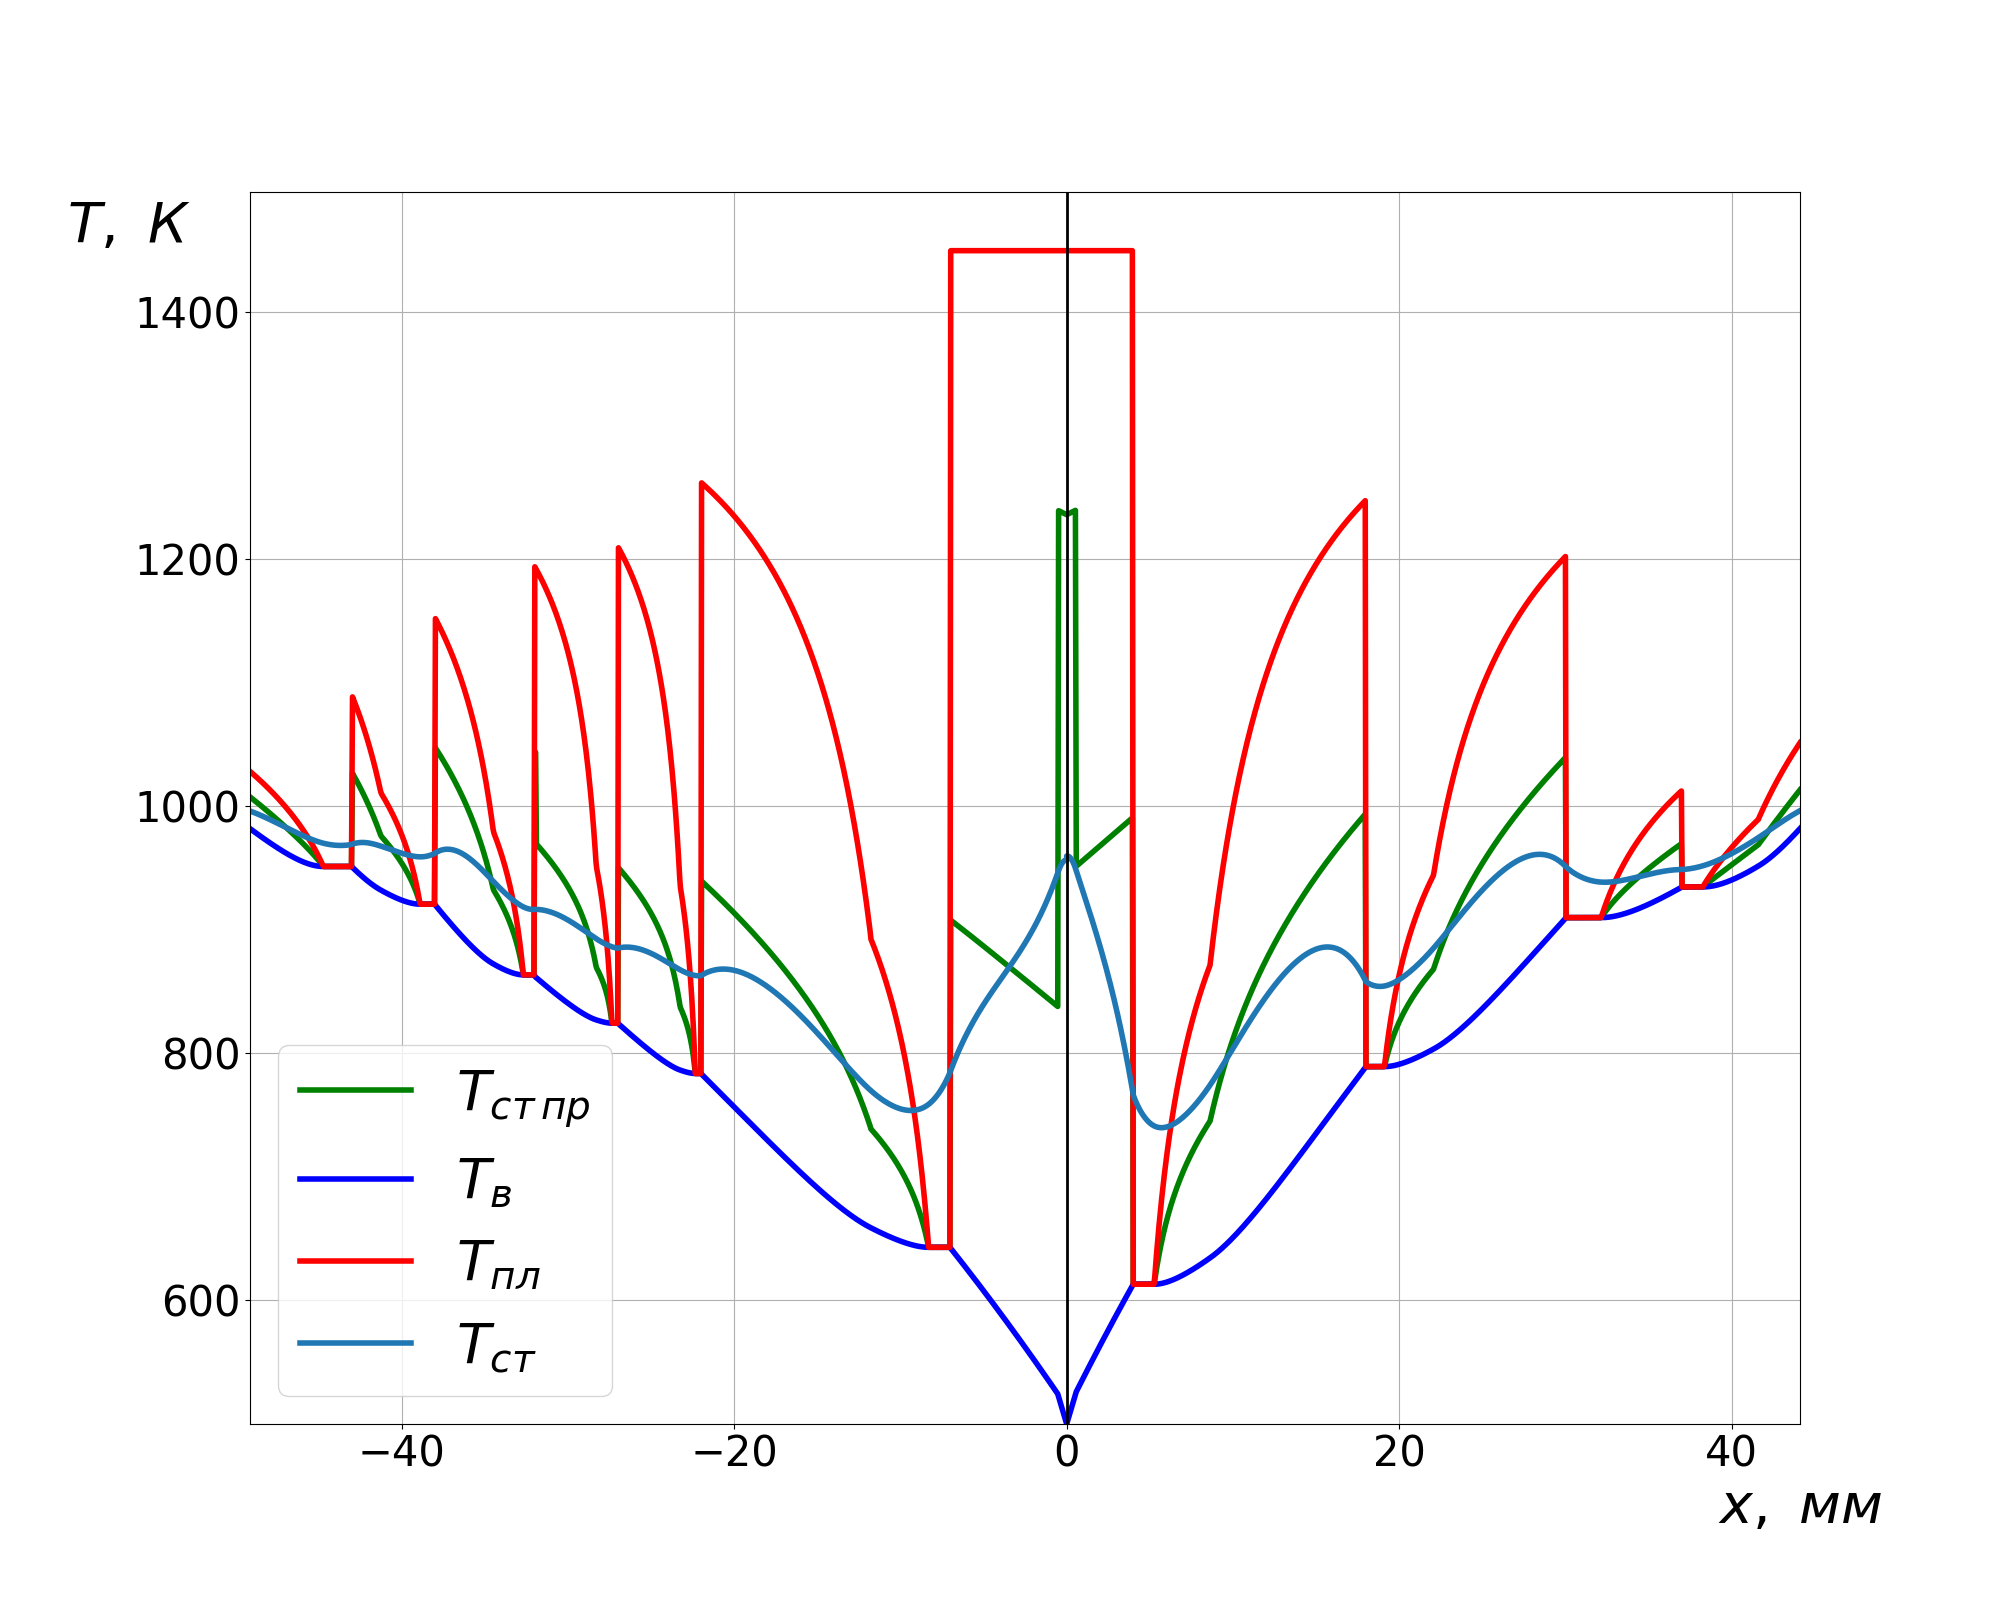
\includegraphics[scale=0.8]{cooling_2_t}
	\caption{Распределение температур газа, воздуха и металла}
\end{figure}

Также был проанализирован вариант без выдува воздуха в лобовой точке (рис. 7). Однако отсутствие выдува в лобовой
точке приводит к сильному перегреву с возможным прогарание профиля лопатки.
\begin{figure}[H]
    \centering
	\includegraphics[scale=0.8]{cooling_2_t_hot}
	\caption{Распределение температур газа, воздуха и металла (без выдува в лобовой кромке)}
\end{figure}

Таким образом, из расчета следует, что ни в одной точке температура материала лопатки не превышает 1100 К (максимальная температура
равна 1081 К), что в случае равномерного поля температур перед сопловыми лопатками обеспечивает достаточную прочность лопаток [1].
Однако основной причиной выхода из строя сопловых лопаток является не температурная деформация, а коррозия.
Для защиты от воздействия агрессивной среды сопловые лопатки покрываются защитным керамическим покрытием на основе
$Zr0_2$ с металлической подложкой на основе $Ni-Cr-Al-Y$. Такой состав покрытия обеспечивает его хорошую адгезию к
основному материалу лопатки и предотвращает его от растрескивания под действием термоциклических нагрузок.
Побочным эффектом применения данного покрытия является снижение температуры основного материала лопатки на 50-60 К
вследствие крайне низкой теплопроводности керамического слоя покрытия.

    \section{Технологическая часть}
    \subsection{Назначение детали в узле. Краткое описание конструкции}
Рассматриваемая деталь – лопатка ротора первой ступени турбины высокого давления (ТВД). Сопловые и рабочие лопатки первой
ступени ТВД образуют газодинамическую решетку, проходя через которую горячий газовый поток передает свою энергию ротору.
Лопатка является охлаждаемой по конвективно-пленочной системе: внутри лопатки выполнена сеть каналов, проходя по которым
охлаждающий воздух принимает теплоту от лопатки, понижая ее температуру. Часть охлаждающего воздуха выдувается в проточную
часть турбины через отверстия на профильной части лопатки для организации защитной воздушной пленки на лопатке.

Лопатка ротора является деталью сложной пространственной формы и конструктивно состоит из трех частей: пера лопатки, хвостовика и полки.

Перо лопатки является деталью со сложной фасонной поверхностью, которая непосредственно взаимодействует с газовым потоком
и преобразует его кинетическую энергию в механическую энергию вращения ротора. От втулки к периферии площадь поперечного
сечения пера лопатки уменьшается. На кромках, а также на спинке и корытце выполнены отверстия. Также в периферийном сечении
выполнены отверстия для выдува воздуха в радиальный зазор.

Данная лопатки имеет трехзубый хвостовик елочного типа, обеспечивающий ее установку и фиксацию на диске в окружном направлении.
В осевом направлении лопатка фиксируется с помощью выступа внизу замковой части, а также с помощью деформируемого замка,
устанавливаемого между диском и канавкой на выходной части полки. Также хвостовик выполняет функцию подвода воздуха к
профильной части лопатки с каналов в его основании.

Полка лопатки разделяет хвостовик и перо, а также обеспечивает гладкость проточной части и изоляцию диска турбины от газового
потока. Полки лопаток стыкуются, образуя непрерывную поверхность вращения.

На входной части полки лопатки имеется выступ, обеспечивающий гладкость переходного участка проточной части статором и
ротором ступени турбины высокого давления.

\begin{longtable}{|p{12cm}|c|}
	\hline
	\textbf{Параметр} & \textbf{Значение} \\ \hline
	\endhead
	Температура торможения в относительном движении на входе в венец & 1306,9 К \\ \hline
	Давление торможения в относительном движении на входе в венец & 1,099 МПа \\ \hline
	Частота вращения ротора & 12000 МПа \\ \hline
	\caption{Условия работы лопатки} \label{tab:technology-env-parameters}
\end{longtable}

В связи с тем, что лопатка подвержена одновременному воздействию высокой температуры и высоких напряжений, материал должен обладать высокой жаропрочностью. Также, поскольку данный двигатель предназначен для эксплуатации в составе привода газоперекачивающего агрегата (ГПА), для него характерна частая смена режимов работы, что в свою очередь требует использования материала с высоким сопротивлением усталости.

В качестве материала для лопатки выбирается никелевый сплав ЖС36, состав которого представлен в таблице 2.

\begin{longtable}{|l|l|}
	\hline
	\textbf{Элемент} & \textbf{Содержание, \%} \\ \hline
	\endhead
	Хром, Cr & 2,5–5,5 \\ \hline
	Кобальт, Co & 5–9,5 \\ \hline
	Алюминий, Al & 5–6,2 \\ \hline
	Титан, Ti & 0,7–1,5 \\ \hline
	Молибден, Mo & 1–4 \\ \hline
	Вольфрам, W & 10,5–13 \\ \hline
	Тантал, Ta & 0,01–4 \\ \hline
	Рений, Re & 1–2,6 \\ \hline
	Ниобий, Nb & 0,7–1,5 \\ \hline
	Иттрий, Y & 0,002–0,075 \\ \hline
	Лантан, La & 0,001–0,05 \\ \hline
	Церий, Ce & 0,001–0,05 \\ \hline
	Празеодим, Pr & 0,002–0,01 \\ \hline
	Неодим, Nd & 0,0002–0,005 \\ \hline
	Гадолиний, Gd & 0,0002–0,005 \\ \hline
	Скандий, Sc & 0,0002–0,005 \\ \hline
	Никель, Ni & основа \\ \hline
	\caption{Состав сплава ЖС36} \label{tab:technology-alloy-properties}
\end{longtable}

\subsection{Анализ технический требований}

К детали предъявлены следующие технические требования:

Отклонение формы контуров корыта и спинки в расчетных сечениях от заданной формы допускается не более 0,1 мм.

Требование назначено из условия обеспечения расчетного режим течения газа.

Невыполнение требования вызовет возникновение нерасчетного режима течения газа, что может привести к следующим негативным последствиям:

Снижение КПД двигателя вследствие неоптимального обтекания лопатки потоком.

Изменение частот вынужденных колебаний лопатки вследствие перераспределения газодинамических сил. Результатом такого изменения может стать быстрый выход лопатки из строя вследствие многоцикловой усталости.

Требования обеспечивают при окончательной обработке поверхностей спинки и корыта с базированием по замку лопатки.
Контроль формы контуров корыта и спинки в расчетных сечениях производится по шаблону (рис. 1).

\begin{figure}[H]
    \centering
    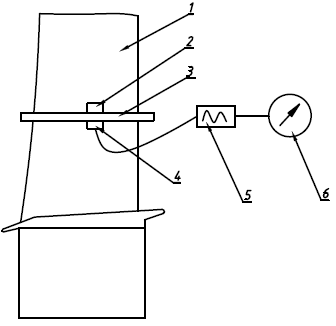
\includegraphics[scale=1]{profile_shape_control}
    \caption{Схема контроля формы профиля лопатки: 1 – лопатка; 2 – светодиод; 3 – шаблон; 4 – фотодиод; 5 – аналого-цифровой преобразователь; 6 – индикатор}
\end{figure}

Допуск на  толщину стенки пера, щелей и перемычек $\pm$ 0,3 мм.

Требования назначено из условия обеспечения расчетного режима охлаждения лопатки.

Увеличение толщины стенок лопатки сверх допуска приводит к уменьшению проходного сечения каналов системы охлаждения, что приводит к уменьшению ее эффективности.

Уменьшение толщины стенок лопатки ниже допуска может привести к прогару стенок и выходу лопатки из строя.

Требование для стенок спинки и корыта обеспечивают при окончательной обработке поверхностей спинки и корыта с базированием по замку лопатки. Требование для внутренних стенок обеспечиваются на этапе изготовления заготовки.
Контроль требования осуществляется ультразвуковым толщиномером (рис. 2).

\begin{figure}[H]
    \centering
    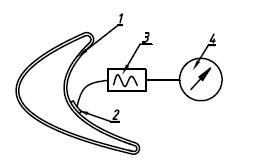
\includegraphics[scale=1]{profile_thk_control}
    \caption{Схема контроля толщины стенок лопатки: 1 – лопатка; 2 – ультразвуковой излучатель/приемник; 3 – аналого-цифровой преобразователь; 4 – индикатор}
\end{figure}

Допуск на толщину замка по впадине третьего зуба 0,06 мм.

Требование назначено из условия обеспечения равнопрочности замковой части лопатки и диска.

Уменьшение толщины замка ниже минимального уровня допуска может привести к недопустимому прослаблению материала лопатки и более быстрому ее изнашиванию. Увеличение толщины замка выше максимального уровня допускам может привести к аналогичным результатам применительно к периферийной части диска.

Данное требование обеспечивают при окончательной обработке поверхностей зубьев замкового соединения с базированием по перу, заключенному в кассету из сплава Вуда.

Контроль требования осуществляется микрометром (рис. 3).

\begin{figure}[H]
    \centering
    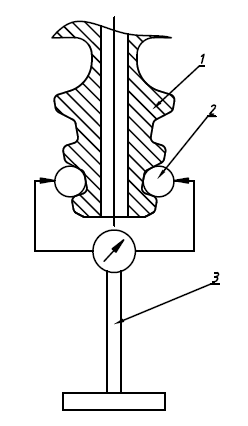
\includegraphics[scale=1]{lock_control}
    \caption{Схема контроля толщины замкового соединения: 1 – замковая часть лопатки; 2 – ролик; 3 – микрометр}
\end{figure}

\subsection{Технологические задачи, возникающие при изготовлении детали}

Основными технологическими задачами, возникающими при изготовлении детали, являются обеспечение качества поверхности профильной части лопатки и обеспечение допусков размеров замковой части лопатки.

К профильной части поверхности лопатки предъявляются высокие требования по обеспечению точности формы профиля и шероховатости поверхности. В связи с этим лезвийная обработка профиля лопатки не допускается. Доводка профиля должно осуществляться только абразивным инструментом.

\subsection{Тип производства и метод работы}

Разработка технологического процесса осуществляется для условий серийного производства. В условиях производства данного типа наиболее целесообразным методом работы является переменно-поточный метод.

Выбор данного метода определяется тем, что использование поточного метода для деталей особой ответственности с множеством контрольных операций затруднительно, а непоточный метод приведет к более низкой загрузке оборудования, удлинит цикл производства и увеличит себестоимость изделия.

\subsection{Технологический анализ конструкции детали}

Конструкция детали состоит из поверхностей сложной пространственной формы, к точности и качеству поверхности которых предъявляются крайне высокие требования.

Перо лопатки образовано трехмерными несимметричными фасонными поверхностями. Также для обеспечения эффективного охлаждения в лопатке выполнена развитая сеть внутренних полостей и 9 рядов отверстий $\diameter$ 0.3 мм на поверхности пера.

Елочный хвостовик лопатки имеет форму призмы с симметричным поперечным сечением сложной формы. В связи со сложной формой профильной части лопатки, при обработке поверхностей хвостовика необходимо использовать специальное приспособление – кассету из сплава Вуда, чтобы обеспечить надежное базирование без риска повредить профильную часть лопатки.

После обработки хвостовик используется в качестве технологической базы для обработки поверхностей пера.

Упрощение геометрических форм лопатки невозможно, так как каждый ее элемент спроектирован для обеспечения эффективного преобразования кинетической энергии потока при соблюдении высоких прочностных свойств конструкции.

Деталь имеет небольшие габариты (40x52x104), что обуславливает сравнительно небольшой объем механической обработки при ее изготовлении. С другой стороны, деталь изготавливается из труднообрабатываемого материала (сплав ЖС36) и является тонкостенной, что не позволяет использовать форсированные режимы обработки.

Вывод: принимая во внимание все вышеперечисленные факторы, стоит признать конструкцию детали нетехнологичной для условий серийного производства. Однако изменение ее конструкции с сохранением эксплуатационных свойств не представляется возможным.

\subsection{Выбор метода изготовления заготовки}
Деталь лопатка в процессе эксплуатации испытывает циклические изгибающие, растягивающие и термоциклические нагрузки. Материал: сталь ЖС-3ВИ. Тип производства: серийное.
Результаты анализа представлены в таблице 3.

\begin{longtable}{|p{6cm}|l|l|}
	\hline
	\textbf{Признак} & \textbf{Значение} & \textbf{\makecell{Приоритетный \\ ряд заготовок}} \\ \hline
	\endhead
	Форма детали & Сложная & О, СК, ОД \\ \hline
	Заготовительные свойства материала & & \\ \hline 
	Жидкотекучесть & Удовлетворительная & О \\ \hline
	Пластичность & Неудовлетворительная & (ОД, П) \\ \hline
	Свариваемость & Неудовлетворительная & (СК) \\ \hline
	Обрабатываемость резанием & Неудовлетворительная & (ОД, П) \\ \hline
	Ориентированность структуры & Необходима & ОД, О \\ \hline
	Удельная стоимость материала & Высокая & О, ОД, ПМ \\ \hline
	Ответственность детали & Высокая & ОД, П \\ \hline 
	Тип производства & Серийное & П, ОД, СК, О \\ \hline
	\caption{Основные признаки, используемые при выборе заготовки} \label{tab:technology-detail-properties}
\end{longtable}

О – отливка; ОД – получение обработкой давлением; П – прокат; СК – сварная или комбинированная; ПМ – полученная методами порошковой металлургии; () – исключение; * - любая (равноприоритетность видов).

Из предварительного анализа следует, что единственным возможным вариантом изготовления лопатки является литье. Данный способ позволяет получить заготовку, максимально приближенную по форме к конечной детали, что немаловажно с учетом высокой стоимости сплава ЖС36. Также, литье является одним из немногих способов получения заготовки, при котором можно изготовить развитую сеть внутренних каналов лопатки (того же эффекта можно достигнуть с помощью порошковой металлургии, но данный способ неприемлем из-за требований к ориентированности структуры заготовки).

В связи с этим, выбирается метод получения заготовки – монокристаллическое литье по выплавляемым моделям. В этом случае точность размеров заготовки достигает 10 квалитета, а шероховатость – значения Ra2,5.

\subsection{Выбор баз и составление маршрутного технологического процесса}

Из-за сложной поверхности пера лопатки и риска ее повреждения, базирование по перу во время обработки хвостовика невозможно. В связи с этим, лопатка помещается в специальное приспособление – кассету и заливается сплавом Вуда. На операциях 005 – 065 базирование производится по поверхностям кассеты. Заготовка лишается шести степеней свободы.

На операциях 085 – 100 базирование производится по профильной (5 степеней свободы) и торцевой (одна степень свободы) поверхностям хвостовика с приложением силы закрепления к противоположному торцу хвостовика. Заготовка лишена шести степеней свободы.
    \section{Организационно-экономическая часть}
    \section{ЧАСТЬ 4. ОРГАНИЗАЦИОННО-ЭКОНОМИЧЕСКАЯ ЧАСТЬ}
\subsection{Оценка единовременных затрат на прототип}
Привод газоперекачивающего агрегата (ГПА) – сложное изделие с чрезвычайно широкой номенклатурой используемых материалов.
Точный расчет по всей номенклатуре крайне затруднителен, а на этапе эскизного проектирования – невозможен. Основной
вклад в затраты вносят дорогостоящие сплавы для горячей части двигателя (гранулированные ЭП741НП, жаропрочные для
охлаждаемых лопаток ЖС6К, ЖС6У, ЖС32) и легкие титановые сплавы для холодной части (ВТ3, ВТ6, ВТ8, ВТ9, АЛ4). Для
сравнительно ненапряженных температурных условий используются хромникелевые и нержавеющие стали и сплавы.

Для упрощения задачи, зная массу прототипа (6650 кг), закладываю коэффициент использования материала КИМ=0,05 и умножаю
на осредненную стоимость материалов (2500 р/кг). Для того, чтобы учесть затраты на оплату труда рабочих, на сумму затрат
на материалы вводится коэффициент 1,5.

Итого, получается стоимость прототипа:
$$
    Ц = 66500,05 \cdot 2500 р/кг \cdot 1,5 = 498750000 руб = 498,75 млн.руб
$$.

\subsection{Оценка снижения затрат в связи с доработкой конструкции}
В научно-исследовательской части настоящей выпускной квалификационной работы была усовершенствована конструкция
компрессора высокого давления: повышены напорности ступеней, в результате чего удалось уменьшить число ступеней с 7 до 5.
Была произведена оценка выигрыша в массе:
\begin{longtable}{|l|l|l|l|l|l|l|}
        \hline
        \textbf{№}&
        \textbf{\makecell{Масса \\ статора, \\ кг}}&
        \textbf{\makecell{Количество \\ лопаток \\ статора}}&
        \textbf{\makecell{Масса \\ лопаток \\ статора}}&
        \textbf{\makecell{Масса \\ ротора, \\ кг}}&
        \textbf{\makecell{Количество \\ лопаток \\ ротора}}&
        \textbf{\makecell{Масса \\ лопаток \\ ротора}}\\\hline
        \endhead
        1 & 23,6 & 23 & 0,3 & 37,1 & 25 & 0,28 \\\hline
        2 & 21,7 & 27 & 0,3 & 38,6 & 29 & 0,29 \\\hline
        \caption{Данные для оценки снижения массы двигателя в сравнении с прототипом} \label{tab:economics-mass-comparison}
    \end{longtable}
Экономия массы в сравнении с прототипом $\Delta m$, кг составила:
$$
    \Delta_m= \left(
        23,6 + 23 \cdot 0,3 + 37,1 + 25 \cdot 0,28
    \right) +
$$
$$
    + \left(
        21,7 + 27 \cdot 0,3 + 38,6 + 29 \cdot 0,29
    \right) = 151,4 \ кг
$$
Можно оценить снижение исходной массы материала для производства установки с учетом коэффициента использования материала:
$$
    \frac{\Delta_m}{КИМ} = \frac{151,4}{0,05} = 3028 \ кг.
$$
Следовательно, снижение затрат на материалы:
$$
    3028 \ кг \cdot 2500 \ р/кг = 7570000 \ руб.
$$
Принимая, что масса остальных деталей и узлов двигателя остается такой же, как в прототипе, вычисляем единовременные
затраты на проектируемый двигатель:
$$
    498750000 - 7570000 = 491180000 \ руб. = 491,18 \ млн.руб.
$$
\subsection{Оценка затрат на единицу мощности}
Одной из важнейших характеристик привода газоперекачивающего агрегата является мощность. С повышением требований к
параметрам цикла двигателя ужесточаются условия работы его узлов и деталей. Применяются сплавы, легированные
дорогостоящими металлами, гранулированные сплавы, повышается трудоемкость изготовления и сборки ДСЕ. Важно оценивать
затраты на единицу мощности. Оценка затрат на единицу мощности представлена в таблице 2
\begin{longtable}{|p{6cm}|c|c|}
    \hline
    \textbf{Параметр} &
    \textbf{Прототип} &
    \textbf{Проектируемый двигатель} \\\hline
    \endhead
    Мощность, МВт & 16 & 16 \\\hline
    Единовременные затраты, млн. руб. & 498,75 & 491,18 \\\hline
    Затраты на единицу мощности, млн. руб./МВт & 31,17 & 30,70 \\\hline
    \caption{Данные для оценки затрат на единицу мощности для прототипа и проектируемого двигателя} \label{tab:economics-unit-power}
    \end{longtable}
Анализ данных, представленных в таблице 2, показывает, что проектируемый двигатель является более выгодным с точки зрения
затрат на единицу мощности по сравнению с прототипом.

\subsection{Расчет затрат на эксплуатацию}
Заложен полный ресурс 100 тыс.ч. Межремонтный интервал – 25 тыс. ч. Затраты на один ремонт составляют 0,25 от единовременных затрат.
Таким образом получим стоимость одного ремонта двигателя $С_{рем}$:
\begin{longtable}{c c}
    Прототип & $498,75 \cdot 0,25=124,69$ млн.руб \\
    Проектируемый двигатель & $491,18 \cdot 0,25=122,80$ млн.руб \\
\end{longtable}
Цена газа для промышленных потребителей $Ц_{топл} = 4316 руб/(тыс \ м^3)$.
Примерный среднечасовой расход топлива проектируемого двигателя
$$
    G_т = 4,422 \ тыс \ м^3 / час.
$$
Можно посчитать среднегодовые затраты на топливо проектируемого двигателя
$$
    С_{топл}=G_т \cdot Ц_{топл} \cdot 8760 = 4,422 \cdot 4316 \cdot 8760 = 167,18 \ млн.руб./год.
$$
А также среднегодовые затраты на топливо прототипа
$$
    С_{топл \ прот} = G_{т \ прот} \cdot Ц_{топл} \cdot 8760 = 4,667 \cdot 4316 \cdot 8760 = 176,45 млн.руб./год.
$$
Введем коэффициент эксплуатационных затрат $К_{эксп} = 0,8$, связывающий среднегодовые затраты на регламентное и
техническое обслуживание и среднегодовые затраты на капитальный ремонт установки. В результате получим среднегодовые
затраты на регламентное и техническое обслуживание установки:
$$
    С_{эксп \ прот} = К_{эксп} \cdot С_{рем \ прот} \cdot 876025000 = 0,8 \cdot 124,69 \cdot 876025000 = 34,95 млн.руб \
$$
$$
    С_{эксп} = К_{эксп} \cdot С_{рем} \cdot 876025000 = 0,8 \cdot 122,80 \cdot 876025000 = 34,42 \ млн.руб.
$$

\begin{figure}[H]
    \centering
    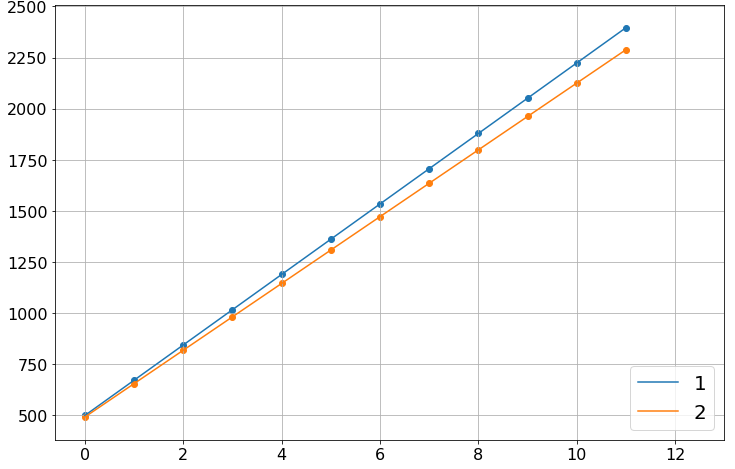
\includegraphics[scale=0.7]{cost}
    \caption{Суммарные затраты на прототип 1 и проектируемый двигатель 2 за 11 лет эксплуатации}
\end{figure}
Проведенная в исследовательской части дипломного проекта оптимизация цикла установки позволяет снизить единовременные
затраты за счет уменьшения стоимости компрессора высокого давления, а использование высокой температуры в камере сгорания
увеличивает экономичность двигателя в целом.
    \section{Охрана труда и экология}
    \section{ОХРАНА ТРУДА И ЭКОЛОГИЯ}
\label{sec:ecology} 

\subsection{Назначение двигателя} 
 \label{sub:ecology_engine_purpose} 

Двигатель предназначен для использования в качестве привода нагнетателя на линейных компрессорных станциях природного газа.

Двигатель выполнен трехвальным со свободной турбиной. 

Мощность – 16 МВт.

Основные части: компрессор низкого давления (КНД), компрессор высокого давления (КВД), камера сгорания (КС), турбина высокого давления (КВД), турбина низкого давления (КНД), силовая турбина (ТС), выходное устройство.

Частоты вращения валов: высокого давления – 12000 об/мин, среднего давления – 9500, низкого давления – 7800 об/мин.

Топливо – природный газ.

Температура газа за камерой сгорания – 1450 К.

\subsection{Анализ вредных и опасных производственных факторов на этапе эксплуатации} % (fold)
 \label{sub:ecology_factor_analisys} 

При эксплуатации двигателя к вредным и опасным факторам относятся:
\begin{itemize}
	\item Повышенный уровень шума на рабочем месте, вызванный всасыванием воздуха, колебанием газа в элементах проточной части, колебанием элементов конструкции из-за вращения ротора, истечения реактивной струи из выходного устройства.
	\item Загрязнение воздуха в области, прилегающей к компрессорной станции, продуктам сгорания топлива, содержащими оксиды азота, углерода, сажу; парами масла из системы смазки (Таблица 5.1).
	\item Повышенный уровень вибраций из-за дисбаланса вращающихся масс (Таблица 5.1).
	\item Повышенный уровень температуры в рабочей зоне вследствие нагрева корпуса двигателя (Таблица 5.1).
	\item Повышенный уровень температур поверхностей оборудования и поверхностей проточной части: в компрессоре за счет сжатия воздуха, в турбине – за счет температуры горячего газа (Таблица 5.1). 
\end{itemize}

Анализ перечисленных факторов представлен в таблице 5.1 с указанием нормативного документа и нормативных значений рассмотренных производственных факторов.

\begin{longtable}{|p{4cm}|p{3cm}|p{5cm}|p{4cm}|}
	\hline
	\textbf{Вредные и опасные производственные факторы ГОСТ 12.2.003-74, Р2.2.2006-05} & 
	\textbf{Источник производственного фактора} &
	\textbf{Нормативное значение} &
	\textbf{Нормативный документ} \\ \hline
	\endhead
	
	Повышенный уровень шума на рабочем месте & 
	Вентилятор, Компрессор, Турбина, Выходное устройство &
	Таблица 2, строка 4 – для рабочих мест за пультами регулирования параметров установки &
	СН 2.2.4/2.1.8.562-96 \\ \hline

	Повышенный уровень продуктов сгорания в воздухе рабочей среды &
	Камера сгорания & 
	Максимальные разовые ПДК: $CO_2 \ (2 \ мг/м^3)$, $CO \ (5 \ мг/м^3)$, $NO_2 \ (10 \ мг/м^3)$, $NO \ (20 \ мг/м^3)$,  &
	ГН2.2.5.3532-18 (таблица 1) "Гигиенические нормативы. Предельно допустимые концентрации (ПДК) вредных веществ в воздухе рабочей зоны" \\ \hline

	Повышенный уровень вибрации & 
	Ротор низкого давления; Ротор среднего давления; Ротор высокого давления &
	Указано в таблице 3 (для технологических вибраций, воздействующих на человека на рабочих местах стационарных машин или передающих на рабочие места, не имеющие источников вибрации) &
	СН 2.2.4/2.1.8.566-96(таблица 6) "Производственная вибрация. Вибрации в жилых и общественных зданиях" \\ \hline

	Микроклимат & 
	Камера сгорания &
	Производственное помещение Категория работ- IIa (175-232Вт) Температура воздуха 20-22 $\degree$С, Температура поверхностей 19-23 $\degree$С, Относительная влажность 60-40 \%, Скорость движения воздуха 0,2 м/с &
	СП 60.13330.2016 "Отопление, вентиляция и кондиционирование" \\ \hline

	Повышенная температура поверхностей оборудования, материалов &
	Корпус турбин; Корпусы камеры сгорания; Корпус выходного устройства &
	51 $\degree$С (1 мин) &
	СанПиН 2.2.3.548-96 Гигиенические требования к микроклимату производственных помещений \\ \hline

	\caption{Анализ вредных и опасных производственных факторов} \label{tab:ecology-factor-analisys}
\end{longtable}

\subsection{Анализ уровня шума на станции} % (fold)
\label{sub:ecology_noise_analisys}

Расчет производился в программном комплексе АРМ «Акустика».

Расчет был произведен для машинного отделения и двух прилегающих комнат – комнаты управления и электротехнического отсека. Схема расчетной области представлена на рис. 5.1. 

\begin{figure}[H]
	\centering
	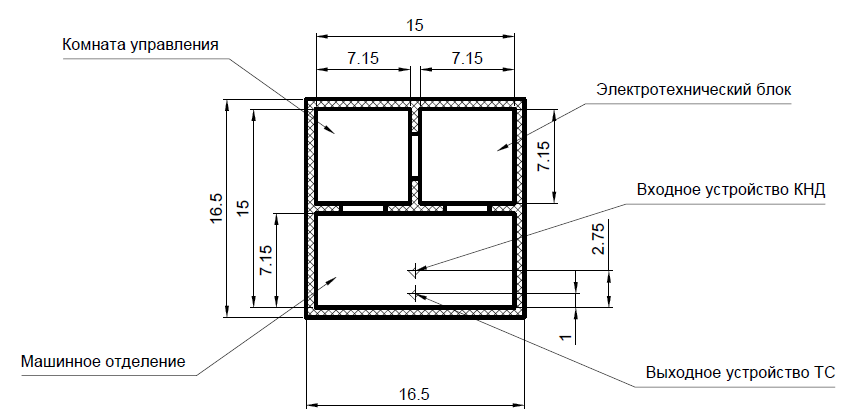
\includegraphics[scale=0.5]{ecology_plan}
	\caption{Схема расчетной области (КНД – компрессор низкого давления, ТС – силовая турбина)}
\end{figure}

Соответствующая модель, построенная в программном комплексе АРМ «Акустика» приведен на рис. 5.2.

\begin{figure}[H]
	\centering
	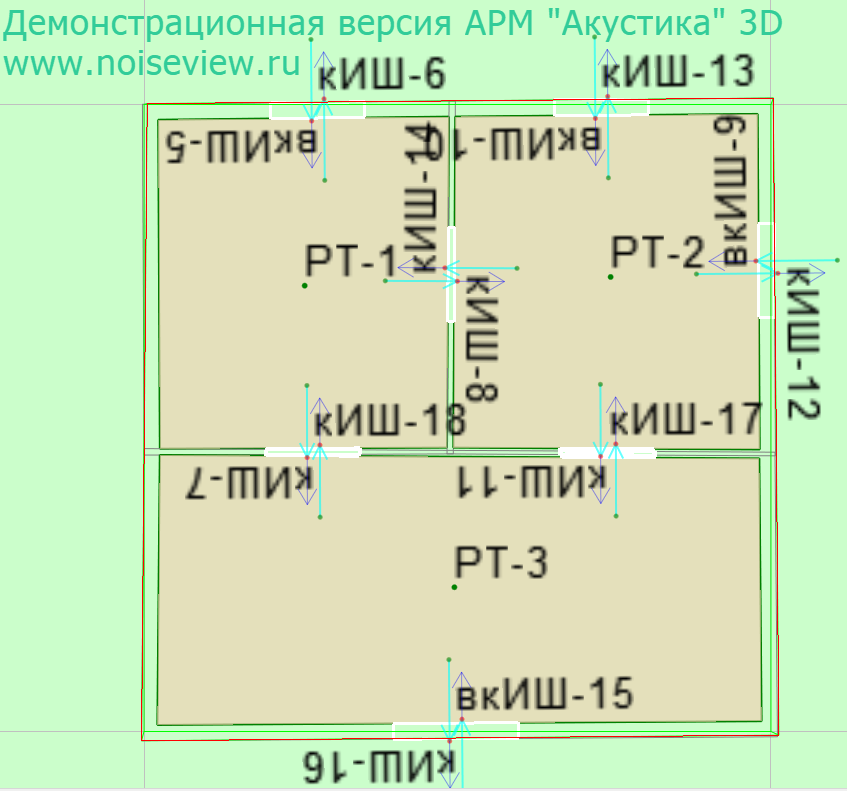
\includegraphics[scale=0.5]{ecology_bc}
	\caption{Расчетная модель, построенная в программном комплексе АРМ "Акустика"}
\end{figure}

Для расчета уровней шума использованы шумовые характеристики вентилятора и выходного устройства двигателя НК38-СТ, идентичные разрабатываемому двигателю. Уровни звукового давления, дБ в октавных полосах со среднегеометрическими частотами, Гц  представлены в таблице 5.2.

\begin{samepage}
\begin{longtable}{|c|c|c|c|c|c|c|c|}
    \hline
    \multicolumn{1}{|c}{}& \multicolumn{7}{c|}{Частота, Гц} \\ \hline
    Источник & 31,5 & 63 & 125 & 250 & 500 & 1000 & 2000 \\ \hline
	Вентилятор & 104 & 102 & 103 & 97 & 97 & 94 & 95 \\ \hline
	Выходное устройство & 119 & 117 & 121 & 116 & 114 & 110 & 115 \\ \hline    
    \caption{Уровни звукового давления, дБ в октавных полосах со среднегеометрическим частотами Гц} \label{tab:ecology_noise_power}
\end{longtable}
\end{samepage}

Изолинии звукового давления, полученные в результате расчета показаны на рис. 5.3.

\begin{figure}[H]
	\centering
	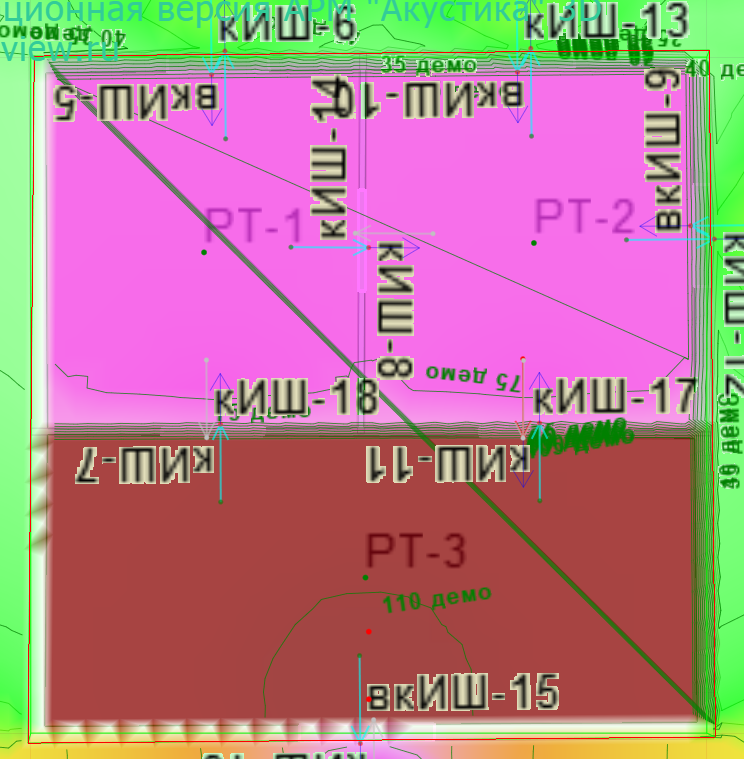
\includegraphics[scale=0.5]{ecology_result}
	\caption{Изолинии звукового давления}
\end{figure}

Сравнение уровней звукового давления в расчетной точке, находящейся в комнате управления с нормативным (согласно СН 2.2.4/2.1.8.562-
96 таблица 2, строка 4) представлено в таблице 5.3.
 
\begin{figure}
\begin{longtable}{|c|c|c|c|c|c|c|c|}
    \hline
    \multicolumn{1}{|c}{}& \multicolumn{7}{c|}{Частота, Гц} \\ \hline
    Источник & 31,5 & 63 & 125 & 250 & 500 & 1000 & 2000 \\ \hline
	Норматив & 103 & 91 & 83 & 77 & 73 & 70 & 68 \\ \hline
	Расчетная точка & 83 & 81,5 & 77,3 & 70,1 & 63,8 & 56,4 & 62,5 \\ \hline   
    \caption{Сравнение полученных уровней звукового давления с нормативным} \label{tab:ecology_noise_norm}
\end{longtable}
\end{figure}

Из полученных данных следует, что уровень шума на рабочем месте, не превышает нормативного ни в одном из частотных диапазонов. 

\subsection{Оценка размера зоны распространения облака горючих газов и паров при аварии} % (fold)
\label{sub:ecology_cloud}
 
Оценка размера зоны распространения облака горючих газов заключается в определении зоны с концентрацией горючего вещества выше нижнего концентрационного предела воспламенения (НКПВ). Для природного газа эта величина равна 29 мг/л.
Исходные данные для проведения расчета приведены в таблице 5.4.

\begin{longtable}{|p{4cm}|p{4cm}|p{4cm}|p{4cm}|}
	\hline
	\textbf{Величина} & 
	\textbf{Обозначение} &
	\textbf{Размерность} &
	\textbf{Значение} \\ \hline
	\endhead

	Температура кипения природного газа & $T_к$ & К & 113 \\ \hline
	Теплоемкость природного газа & $C_{pг}$ & $Дж/(кг \cdot К)$ & 3074 \\ \hline
	Теплоемкость воздуха & $C_{pг}$ & $Дж/(кг \cdot К)$ & 1006 \\ \hline
	Газовая постоянная воздуха & $R_в$ & $Дж/(кг \cdot К)$ & 287 \\ \hline
	Газовая постоянная природного газа & $R_в$ & $Дж/(кг \cdot К)$ & 519,6 \\ \hline
	Атмосферное давление & $p_а$ & Па & $1,013 \cdot 10^5$ \\ \hline
	Атмосферная температура & $T_а$ & К & 288 \\ \hline
	Теплота парообразования природного газа & $L_г$ & Дж/кг & $510 \cdot 10^3$ \\ \hline
	Теплота парообразования водяных паров & $L_в$ & Дж/кг & $2256 \cdot 10^3$ \\ \hline
	Температура подстилающей поверхности & $T_{пов}$ & К & 300 \\ \hline
	Относительная влажность & $\psi$ & \% & 50 \\ \hline
	Массовая доля водяных паров & $X$ & - & $9,35 \cdot 10^{-3}$ \\ \hline
	Температура газа в трубопроводе & $T_г$ & К & 275 \\ \hline
	Диаметр трубопровода & $D$ & м & 1,2 \\ \hline
	Длина участка трубопровода между отсечными клапанами & $L$ & м & 6 \\ \hline
	Давление газа в трубопроводе & $p_г$ & Па & $5,6 \cdot 10^6$ \\ \hline	
	\caption{Исходные данные для проведения оценки зоны распространения облака горючих газов и паров при аварии} \label{tab:ecology-cloud-input}
\end{longtable}

Определим массу газа между отсечными клапанами $m_г$, кг:
$$
	m_г = \frac{
		p_г
	}{
		R_г T_г
	} \cdot \frac{\pi}{4} \cdot D^2 L = \frac{
		5,4 \cdot 10^6
	}{
		519,6 \cdot 275
	} \cdot \frac{3,14}{4} \cdot 1,2^2 \cdot 6 = 265,8 кг.
$$
Определим массу воздуха, мгновенно вовлекающуюся в облако углеводородов , кг:
$$
	m_в = \frac{
		(1 - \delta) \cdot m_г \cdot L_г
	}{
		C_{pв} \cdot (T_в - T_г) + XL_в
	},
$$
где
$$
	\delta = 1 - exp\left( 
		-\frac{
			C_{pг}(T_в - T_к)
		}{
			L_г
		} 
	\right) = 1 - exp\left( 
		-\frac{
			1006 \cdot (288 - 133)
		}{
			510 \cdot 10^3
		}
	\right) = 0,65,
$$
таким образом,
$$
	m_в = \frac{
		(1 - 0,65) \cdot 265,8 \cdot 510 \cdot 10^3
	}{
		1006 \cdot (288 - 133) + 9,35 \cdot 10^{-3} \cdot 2256 \cdot 10^3 \ кг.
	},
$$
Принимается, что образовавшееся облако дрейфует по ветру со скоростью $w_о = 0,6 w$, где $w$ – скорость ветра, и имеет в начальный момент форму цилиндра, высота которого равна его радиусу. С течением времени высота облака уменьшается, а радиус растет.

Скорость ветра зависит от класса устойчивость по Паскуиллу. В данном расчете принимается класс по Паскуиллу B, что соответствует наиболее опасному случаю – наибольшему распространению углеводородного облака. Соответствующая этому классу устойчивости скорость ветра $w = 2 \ м/с$.
Изменение во времени радиуса, высоты облака и концентрации газа в нем в начальной фазе (фаза падения) определяется путем решения систем обыкновенных дифференциальных уравнений:

\[
\left\{
	\begin{array}{ll}
	  \frac{dm_в}{dt} = \rho_в \pi r^2 a_2 a_3 w Ri^{-1} + 2 \rho_в a_1 \frac{dr}{dt} \pi r h \\
	  \frac{dT}{dt} = \frac{
	  	\frac{dm_в}{dt} C_{pв} (T_в - T) + \pi r^2 \cdot (T_{пов} - T)^{1,333}
	  }{
	  	m_в C_{pв} + m_г C_{pг}
	  }\\
	  \frac{dr}{dt} = a_4 \left(
	  	\frac{
	  		dh \cdot (\rho_{г.в.} - \rho_в)
	  	}{
	  		\rho_{г.в.}	
	  	}
	  \right)^{0,5}
	\end{array}
\right.
\]
где $m_в$, кг – масса воздуха в облаке, $\rho_в, \ кг/м^3$ – плотность воздуха, $r, \ м$ – радиус облака, $a_1, a_2, a_3, a_4$ – коэффициенты ($a_1=0,7, \ a_2=0,5, \ a_3=1,07, \ a_4=0,3$), $g, \ м/с$ – ускорение свободного падения;
 
 $Ri$ – число Ричардсона, определяемое из соотношения:
$$
	Ri = \frac{
		\left(
			\frac{
				5,88h^{0,48}g
			}{
				a_3^2 w^2
			}
		\right)^{0,5}
		(\rho_{г.в.} - \rho_в)
	}{\rho_в};
$$
$h, \ м$ – высота облака, $T, \ к$ – температура облака, $\rho_{г.в.}, \ кг/м^3$ – плотность паровоздушного воздуха.
Для решения системы уравнений необходимо дополнительное соотношение:
$$
	\rho_{г.в.} = \frac{
		m_в + m_г
	}{
		\left(
			m_в + m_г
		\right)
		\left(
			\frac{T_в}{T}
		\right)
	}.
$$
В качестве критерия окончания фазы падения принимается выполнение условие
$$
	\frac{\rho_{г.в.} - \rho_в}{\rho_{г.в.}} < 10^{-3}.
$$
Зависимость $h=h(t)$ определяется из соотношения:
$$
	h(t) = \left(
		m_в + m_г
	\right)
	\left(
		\frac{T_в}{T}
	\right)
	\frac{
		1
	}{
		\pi r(t)^2
	}
$$
Концентрация газа в точке с координатами  определяется по формуле:
$$
	C(x, y, z) = \frac{
		2m_г
	}{
		(2\pi)^{1,5} \cdot \sigma_y^2 \cdot \sigma_z^2
	} \cdot 
	exp\left(
		-\frac{
			(x - x_0)^2 + y^2
		}{
			2\sigma_y^2
		}
	\right) \cdot
	exp\left(
		-\frac{
			z^2
		}{
			2\sigma_z^2
		}
	\right)
$$
где $\sigma_y, \ \sigma_z$ – среднеквадратичные отклонения, зависящие от величины $x_c - x_0$; $x_c, \ м$ – координата центра облака в направлении ветра; $x_0, \ м$ – координата точки окончания фазы падения.

При $x_c = x_0$ принимается $\sigma_{y0}=r/2,14$, $\sigma_{z0}=h/2,14$; 

при $x_c \neq x_0$ $\sigma_y^2 = \sigma_{y0}^2 + \sigma_y(x_c - x_0)$, $\sigma_z^2 = \sigma_{z0}^2 + \sigma_z(x_c - x_0)$.

Результатом расчета является пространственное распределение концентраций углеводородного облака. Срез такого распределения на уровне земли ($z=0$) представлен на рис. 5.4.

\begin{figure}[H]
	\centering
	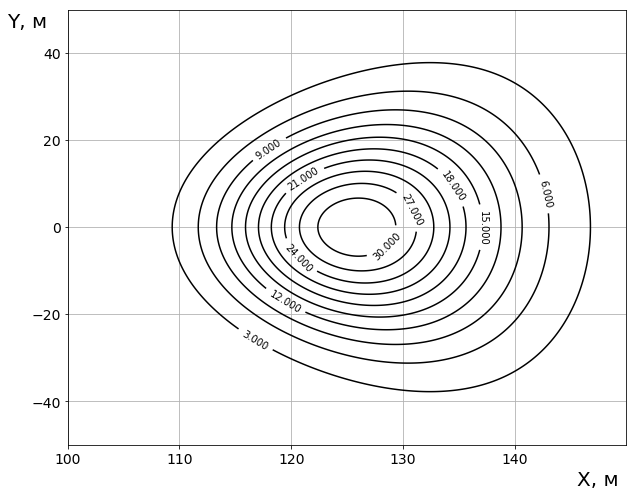
\includegraphics[scale=0.75]{ecology_cloud}
	\caption{Срез распределения концентраций на момент окончания фазы падения}
\end{figure} 

Из полученного решения видно, что зона воспламенения по мере движения облака распространяется вплоть до расстояния 130 м по направлению ветра. Следовательно, открытый огонь недопустим в радиусе 130 м от станции.

    \section*{ЗАКЛЮЧЕНИЕ}
\addcontentsline{toc}{section}{ЗАКЛЮЧЕНИЕ}

Спроектирована газотурбинная установка мощностью 16 МВт для использования на линейных
компрессорных станциях магистральных газопроводов.

В научнои исследовательской части работы проведено анализ различных схем установки в широком
диапазоне рабочим мощностей, а также проведена оптимизация системы охлаждения, позволившая при уменьшении
расхода охлаждающего воздуха снизить неравномерность поля температур в сопловом аппарате
турбины высокого давления с 256,7 до 141,4 К без увеличения максимальной температуры металла.

В конструкторской части проекта проведены расчет основых узлов установки (компрессор низкого давления, компрессор высокого давления,
камера сгорания, турбина высокого давления, турбина низкого давления, силовая турбина) и разработана
конструкия узлов и компоновка установки на станции.

В технологическоц части разработа маршрутный технологический процесс изготовления рабочей лопатки турбины высокого давления.

В организационно-экономической части работы посчитана стоимость проктного варианта двигателя и проведено сравнение прямых
эксплуатационных расходов проектного варианта двигателя с установкой ГПА-16 <<Ладога>>.

Выполнен анализ вредных и опасных производственных факторов установки на этапе эксплуатации. Проведен расчет шума двигателя на
номинальном режим, а также определена зона поражения в случае утечки газа со станции.

    %\section*{Список использованных источников}
%\addcontentsline{toc}{section}{Список использованных источников}
\begin{thebibliography}{99}
    \bibitem{heat_exchangers} Теплообменные аппараты и системы охлаждения газотурбинных и комбинированных установок: учебник для
    вузов / Иванов В. Л., Леонтьев А. И., Манушин Э. А., Осипов М. И. ; ред. Леонтьев А. И. - 2-е изд.,
    стер. - М. : Изд-во МГТУ им. Н. Э. Баумана, 2004. - 591 с. : ил. - Библиогр.: с. 576-577. - ISBN 5-7038-2138-X.
    \bibitem{js_36_properties} Голубовский Е.Р., Светлов И.Л., Хвацкий К.К. Длительная прочность никелевых сплавов для
    монокристаллических лопаток газотурбинных установок // Журнал <<Конверсия в машиностроении>>. - 2005. - №3.
    \bibitem{gtd_theory_text_book} Теория и проектирование газотурбинных и комбинированных установок: учебник для вузов
    / Манушин Э.А., Михальцев В.Е., Чернобровкин А.П. - М. : Изд-во МГТУ им. Н.Э. Баумана, 1997.
    \bibitem{gtd_oil_and_gas} Б.П. Поршаков, А.А. Апостолов, В.И. Никишин. Газотурбинные установки: -М: ГУП Издательство
    «Нефть и газ» РГУ нефти и газа им. И.М. Губкина, 2003. – 240 с.
    \bibitem{gtd_tomsk} Рудаченко А.В. Газотурбинные установки для транспорта природного газа: учебное пособие второе издание
    переработанное: учебное пособие / А.В. Рудаченко, Н.В. Чухарева; Томский политехнический университет. – Томск:
    Изд-во Томского политехнического университета, 2012. – 213 с.
    \bibitem{cycle_methodics} Михальцев, В.Е. Расчет параметров цикла при проектировании газотурбинных двигателей и комбинированных установок : учеб. пособие / В.Д. Моляков, ред.: И.Г. Суровцев, В.Е. Михальцев .— Новосибирск : Изд-во НГТУ, 2014 .— 60 с. — ISBN 978-5-7038-3814-3.
    \bibitem{shlyakhtenko} Шляхтенко С.М., Сосунов В.А. Теория двухконтурных турбореактивных двигателе – М.: Машиностроение, 1979. – 432с.
    \bibitem{comp_char} Ланшин А.И., Зудов С.М., Умнов Е.И. Алгоритм обобщенного представления характеристик свехзвуковых
    компрессоров при математическом моделировании двигателей высокоскоростных летательных аппаратов. // Вопросы авиационной науки и техники. 1995. №2. С. 52–61.
    \bibitem{kazandjan} Теория авиационных двигателей. Теория лопаточных машин: Учебник для студентов, обучающихся по специ­альности
    «Эксплуатация летательных аппаратов и двигателей». /Под ред. П. К. Казанджана.— М.: Машиностро­ение, 1983.— 217 с., ил.
    \bibitem{radial_compressors} Ивановский Н.Н., Криворотько В.Н. Центробежные нагнетатели природного газа: Учебн. пособие для техникумов.
    – М.: Недра, 1994. – 176 с.: ил.
    \bibitem{mikhaltsev_1} В.Е. Михальцев, В.Д. Моляков. Теория и проектирование газовой
    турбины: Учеб. пособие по курсу «Лопаточные машины газотурбинных и
    комбинированных установок. Газовые турбины». – Ч.1: Теория и
    проектирование ступени газовой турбины / под ред. М.И. Осипова. – М.: Изд-во
    МГТУ им. Н.Э. Баумана, 2006. – 104 с.
    \bibitem{mikhaltsev_2} В.Е. Михальцев, В.Д. Моляков. Теория и проектирование газовой
    турбины: Учеб. пособие по курсу «Лопаточные машины газотурбинных и
    комбинированных установок. Газовые турбины». – Ч.2: Теория и
    проектирование многоступенчатой газовой турбины / под ред. М.И. Осипова. -
    М.: Изд-во МГТУ им. Н.Э. Баумана, 2008. – 116 с.
    \bibitem{ivanov} В.Л. Иванов. Воздушное охлаждение лопаток газовых турбин :
    Учеб. пособие по курсу «Системы охлаждения газотурбинных двигателей,
    газотурбинных и комбинированных установок» / под ред. М. И. Осипова – М.:
    Изд-во МГТУ им. Н.Э. Баумана, 2013. – 94 с.
    \bibitem{beknev} В.С. Бекнев. Расчет осевого компрессора. Методические указания
    по выполнению курсовых и дипломных проектов; под ред. Р.З. Тумашева. М.:
    Изд-во МГТУ им. Н.Э. Баумана, 1981. – 39 с.
    \bibitem{kondakov} А.И. Кондаков. Курсовое проектирование по технологии
    машиностроения. – М.: КНОРУС, 2012. – 400 с.
\end{thebibliography}

\end{document}
